% Commenti speciali

% !TEX encoding = UTF-8 Unicode
% !TEX TS-program = pdflatex
% !TeX spellcheck = it_IT
% !TEX root = Dispensa/afed.tex

% Capitolo 1
\chapter{Spazi di Sobolev}
\section{Prime proprietà degli spazi di Sobolev}
\begin{definizione}
	Chiamiamo $W^{1,1}_{loc}(U)$\index[simboli]{$W^{1,1}_{loc}(U)$} l’insieme delle $u \in L^{1}_{loc}(U)$ per cui esistono $v_{1},\dots,v_{n} \in L^{1}_{loc}(U)$ tali che per ogni $j = 1,\dots, n$, per ogni $\varphi \in C^{\infty}_{c}(U)$ risulta
	\[ \int_{U} uD_{j}\varphi d\mathcal{L}^n = - \int_{U}v_{j}\varphi d\mathcal{L}^n.\]
\end{definizione}
\begin{osservazione}\label{derivatadebolecasoregolare}
	Se $u \in C^{1}(U)$, allora per ogni $j = 1,\dots, n$ $D_{j}u \in C(U)$ e per la Formula di Gauss--Green
	\[ \int_{U} uD_{j}\varphi d\mathcal{L}^n = - \int_{U}D_{j}u\varphi d\mathcal{L}^n.\]
\end{osservazione}
\begin{proposizione}
	Sia $u \in L^{1}_{loc}(U)$ tale che esistono $v_{1},\dots,v_{n} \in L^{1}_{loc}(U)$ tali che per ogni $j = 1,\dots, n$, per ogni $\varphi \in C^{\infty}_{c}(U)$ risulta
	\[ \int_{U} uD_{j}\varphi d\mathcal{L}^n = - \int_{U}v_{j}\varphi d\mathcal{L}^n.\]
	Allora per ogni $j = 1,\dots, n$, $v_{j}$ è unica in $L^{1}_{loc}(U)$.
\end{proposizione}
\begin{proof}
	Fissato $j$, supponiamo esistano $v_{j}, \hat{v}_{j}$ soddisfacenti le ipotesi. Allora per ogni $\varphi \in C^{\infty}_{c}(U)$
	\[ \int_{U}v_{j}\varphi d\mathcal{L}^n = \int_{U}\hat{v}_{j}\varphi d\mathcal{L}^n \]
	da cui 
	\[ \int_{U}(v_{j} - \hat{v}_{j})\varphi d\mathcal{L}^n = 0 \]
	e quindi $v_{j} = \hat{v}_{j}$ q.o. da cui l'unicità.
\end{proof}

\begin{definizione}\index[analitico]{derivata!debole}
	Chiamiamo le $v_{1},\dots,v_{n}$ sopra introdotte \emph{derivate deboli} o derivate distribuzionali, o derivate variazionali.
\end{definizione}
In particolare, per l'Osservazione \eqref{derivatadebolecasoregolare} denotiamo le derivate deboli con lo stesso simbolo delle derivate ordinarie.
\begin{esempio}
	Sia $U = \left] 0,2\right[ $ e 
	\[ u(x) = \begin{cases}
		x & \textup{se } 0 < x \leq 1, \\
		1 & \textup{se } 1 < x < 2.
	\end{cases} \]
	Mostriamo che $u \in W^{1,1}_{loc}(0,2)$. Consideriamo l'applicazione
	\[ v(x) = \begin{cases}
		1 & \textup{se } 0 < x \le 1, \\
		0 & \textup{se } 1 < x < 2.
	\end{cases} \]
	Per ogni $\varphi \in C^{\infty}_{c}(0,2)$, osservando che $\varphi(2) = 0 $,
	\[ \int_{0}^{2} u \varphi' d\mathcal{L}^1 = \int_{0}^{1}x\varphi'(x)dx + \int_{1}^{2}\varphi'(x)dx = - \int_{0}^{1}\varphi(x)dx = - \int_{0}^{2}v(x)\varphi(x)dx,  \]
	allora $v$ è la derivata debole di $u$.
\end{esempio}
\begin{esempio}
	Sia $U = \left] 0,2\right[ $ e
	\[ u(x) = \begin{cases}
		x & \textup{se } 0 < x \leq 1, \\
		2 & \textup{se } 1 < x < 2.
	\end{cases} \]
	Supponiamo, per assurdo, che esista $v \in L^1_{loc}(0,2)$ tale che per ogni $\varphi \in C^{\infty}_{c}(0,2)$
	\[ \int_{0}^{2}u\varphi'd\mathcal{L}^1 = - \int_{0}^{2}v\varphi d\mathcal{L}^1. \]
	Innanzitutto,
	\[ \int_{0}^{2}u\varphi'd\mathcal{L}^1 = -\int_{0}^{1}\varphi d\mathcal{L}^1 - \varphi(1). \]
	Si può costruire\footnote{Data $\eta \in C^{\infty}_{c}(0,2)$, basta considerare
		\[ \varphi_h(x) = \eta(x)e^{-\abs{x-1}h}. \]} $(\varphi_h) \in C^{\infty}_{c}(0,2)$ tale che $0 \le \varphi_h \le 1$, $\varphi_h(1) = 1$ e $\varphi_h(x) \to 0$ se $x \ne 1$. Allora,
	\[ \int_{0}^{2}v\varphi_h d\mathcal{L}^1 = \int_{0}^{1}\varphi_hd\mathcal{L}^1 + \varphi_h(1)\]
	e dal Teorema della convergenza dominata otteniamo $0=1$, assurdo.
\end{esempio}
\begin{notazione}
	Sia $p \in \left[ 1,\infty\right] $. Indichiamo con  $W^{1,p}(U)$\index[simboli]{$W^{1,p}(U)$} l'insieme delle $u \in W^{1,1}_{loc}(U)$ tali che $u \in L^p(U)$ e per ogni $j = 1,\dots,n$ si ha $D_{j}u \in L^p(U)$.
\end{notazione}

\begin{esempio}\label{Esempiopalla}
	Consideriamo $U= \textup{B}(0,1)$ in $\R^n$, $\alpha > 0$, $p \in \left]
	1,n\right[$ e 
	\[ u(x)=\frac{1}{\abs{x}^\alpha}. \]
	Mostriamo che $u \in W^{1,p}(U)$ se e solo se $\alpha < \frac{n-p}{p}$.
	
	Innanzitutto, per $x \ne 0$, $u$ è regolare e 
	\[ D_ju(x) = -\alpha\frac{x_i}{\abs{x}^{\alpha+2}}, \]
	per cui candidiamo come derivata debole proprio $D_ju$ opportunamente estesa.
	
	Sia ora $\varepsilon > 0$. Senza perdita di generalità, possiamo supporre $\varepsilon < 1$. Consideriamo l'insieme $U_{\varepsilon} = U\setminus \textup{B}(0,\varepsilon) $. Se $\varphi \in C^\infty_{c}(U)$,
	\[ \int_{U_{\varepsilon}} uD_j\varphi d\mathcal{L}^n = - \int_{U_{\varepsilon}} D_ju \varphi d\mathcal{L}^n + \int_{\partial\textup{B}(0,\varepsilon)} u\varphi \nu^j d\mathcal{H}^{n-1}. \]
	Osserviamo che 
	\[ \int_{U} \abs{u}^pd\mathcal{L}^n = K \int_{0}^{1}\frac{1}{\rho^{\alpha p}}\rho^{n-1}d\rho < +\infty \]
	e 
	\[ \int_{U} \abs{Du}^pd\mathcal{L}^n = K \int_{0}^{1}\frac{1}{\rho^{(\alpha+1) p}}\rho^{n-1}d\rho < +\infty \]
	se e solo se $\alpha < \frac{n-p}{p}$. 
	Inoltre, per $\alpha < n-1$, 
	\begin{align*}
		\abs*{\int_{\partial\textup{B}(0,\varepsilon)} u\varphi \nu^j d\mathcal{H}^{n-1}} &\le \varepsilon^{-\alpha}\int_{\partial\textup{B}(0,\varepsilon)} \abs{\varphi} d\mathcal{H}^{n-1} \le \\
		&\le \norm{\varphi}_{\infty}\varepsilon^{-\alpha}\mathcal{H}^{n-1}(\partial\textup{B}(0,\varepsilon)) \le C \varepsilon^{n-1-\alpha} \to 0.
	\end{align*} 
	A questo punto, per il Teorema della convergenza dominata combinato con il fatto che $\chi_{U_{\varepsilon}} \to \chi_{U}$ \emph{q.o.} in $U$,
	\[ \int_{U_{\varepsilon}} uD_j\varphi d\mathcal{L}^n \to  \int_{U} uD_j\varphi d\mathcal{L}^n \]
	e 
	\[ \int_{U} D_ju \varphi d\mathcal{L}^n \]
	che permettono di concludere che $u \in W^{1,p}(U)$ se e solo se $\alpha < \frac{n-p}{p}$.
\end{esempio}

\begin{definizione}
	Siano $k \in \N\setminus\left\lbrace 0\right\rbrace $ e $1\le p \le \infty$. Chiamiamo \emph{spazio di Sobolev}\index[analitico]{spazio!di Sobolev} l'insieme $W^{k,p}(U)$\index[simboli]{$W^{k,p}(U)$} delle $u \in L^1_{loc}(U)$ tali che per ogni multi indice $\alpha \in \N^n$, esiste $v_{\alpha} \in L^p(U)$, detta \emph{$\alpha$-esima derivata debole}, tale che per ogni $\varphi \in C^\infty_c(U)$
	\[ \int_{U}uD^\alpha\varphi d\mathcal{L}^n = (-1)^{\abs{\alpha}}\int_{U}v_{\alpha}\varphi d\mathcal{L}^n. \]
\end{definizione}

\begin{notazione}
	Indichiamo con $H^{1}(U) = W^{1,2}(U)$\index[simboli]{$H^{1}(U)$}.
\end{notazione}

\begin{proposizione}\label{propderivatedeboli}
	Siano $k \in \N\setminus\left\lbrace 0\right\rbrace $, $1 \le p \le \infty$ ed $u,v \in W^{k,p}(U)$.  Valgono i seguenti fatti:
	\begin{enumerate}[$(a)$]
		\item se $\alpha, \beta \in \N^n$ tali che $\abs{\alpha} + \abs{\beta} \le k$, allora $D^\alpha u \in W^{k - \abs{\alpha},p}(U)$ e 
		\[ D^\beta (D^\alpha u) = D^\alpha (D^\beta u) = D^{\alpha + \beta} u;  \]
		\item per ogni $\lambda,\mu \in \R$, $\lambda u + \mu v \in W^{k,p}(U)$ e se $\alpha \in \N^n$ tale che $\abs{\alpha}\le k$,
		\[ D^\alpha (\lambda u + \mu v )= \lambda D^\alpha u + \mu D^\alpha v. \]
		In particolare, $W^{k,p}(U)$ è uno spazio vettoriale su $\R$;
		\item se $V$ è un sottoinsieme aperto di $U$, allora $u \in W^{k,p}(V)$;
		\item  se $\eta \in C^\infty_c(U)$, allora $\eta u \in W^{k,p}(U)$ e se $\alpha \in \N^n$ tale che $\abs{\alpha}\le k$,
		\[ D^\alpha(\eta u) = \sum_{\beta \le \alpha}^{} \binom{\alpha}{\beta} D^\beta \eta D^{\alpha - \beta} u. \qquad \textup{(Formula di Leibniz)} \]
		In particolare, se $\abs{\alpha} = 1$, 
		\[ D^\alpha(\eta u) = u D^\alpha \eta + \eta D^\alpha u. \]
	\end{enumerate}
\end{proposizione}
\begin{proof}\hfill
	\par\noindent
	$(a)$ Innanzitutto, per definizione, per ogni $\eta \in C^\infty_c(U)$
	\[ \int_{U} u D^\alpha \eta d\mathcal{L}^n = (-1)^{\abs{\alpha}} \int_{U} D^\alpha u \eta d\mathcal{L}^n. \]
	Se $\varphi \in C^\infty_c(U)$, allora $D^\beta \varphi \in C^\infty_{c}(U)$ e quindi
	\begin{align*}
		\int_{U} D^\alpha u D^\beta \varphi d\mathcal{L}^n &= (-1)^{\abs{\alpha}} \int_{U}  u D^{\alpha + \beta} \varphi d\mathcal{L}^n = \\ 
		& =(-1)^{\abs{\alpha}} (-1)^{\abs{\alpha} + \abs{\beta}} \int_{U} D^{\alpha + \beta} u \varphi  d\mathcal{L}^n = (-1)^{\abs{\beta}} \int_{U} D^{\alpha + \beta} u \varphi  d\mathcal{L}^n
	\end{align*}
	da cui $D^\beta(D^\alpha u) = D^{\alpha + \beta} u$. Scambiando $\alpha$ e $\beta$ si giunge alla conclusione.
	\par\noindent
	$(b)$ Discende dalla linearità dell'integrale.
	\par\noindent
	$(c)$ Evidente.
	\par\noindent
	$(d)$ Vediamo il caso $\abs{\alpha} = 1$, il caso generale può essere ricavato per induzione. Sia $\varphi \in C^\infty_c(U)$, allora
	
	\[ \int_{U} \eta u D^\alpha \varphi d\mathcal{L}^n  =\int_{U} \left( u D^\alpha(\eta \varphi) - u (D^\alpha \eta)\varphi\right) d\mathcal{L}^n =- \int_{U}\left( \eta D^\alpha u + uD^\alpha \eta\right) \varphi d\mathcal{L}^n.  \qedhere \]
	
\end{proof}

\begin{definizione}
	Siano $k \in \N\setminus\left\lbrace 0\right\rbrace $, $1 \le p \le \infty$ ed $u \in W^{k,p}(U)$. Poniamo 
	\[ \norm{u}_{W^{k,p}(U)} = \begin{cases}
		\left( \displaystyle \sum_{\abs{\alpha} \le k} \norm{D^\alpha u}_{L^p(U)}^p\right) ^{\frac{1}{p}} & 1 \le p < \infty, \\
		\displaystyle \sum_{\abs{\alpha} \le k} \norm{D^\alpha u}_{L^\infty(U)} & p=\infty.
	\end{cases} \]
	In particolare, se $k = 1$,\footnote{Alle volte useremo invece la norma equivalente
		\[ \norm{u}_{W^1,p(U)} = \begin{cases}
			\left( \norm{u}_{L^p(U)}^p + \norm{D u}_{L^p(U)}^p\right) ^{\frac{1}{p}} & 1 \le p < \infty, \\
			\norm{u}_{L^\infty(U)} + \norm{D u}_{L^\infty(U)} & p=\infty,
		\end{cases} \]
		dove con $\norm{D u}_p$ si intende, per ogni $p \in [1,\infty]$, la norma della funzione scalare $\abs{Du}$.} 
	\[ \norm{u}_{W^{1,p}(U)} = \begin{cases}
		\left( \norm{u}_{L^p(U)}^p + \displaystyle \sum_{j = 1}^{n}\norm{D_j u}_{L^p(U)}^p\right) ^{\frac{1}{p}} & 1 \le p < \infty, \\
		\norm{u}_{L^\infty(U)} + \displaystyle \sum_{j = 1}^{n}\norm{D_j u}_{L^\infty(U)} & p=\infty. 
	\end{cases} \]
	
\end{definizione}

\begin{teorema}
	Siano $k \in \N\setminus\left\lbrace 0\right\rbrace $ e $1\le p \le \infty$.	Valgono i seguenti fatti:
	\begin{enumerate}[$(a)$]
		\item $(W^{k,p}(U), \norm{\;}_{W^{k,p}(U)})$ è uno spazio normato su $\R$;
		\item $(W^{k,p}(U), \norm{\;}_{W^{k,p}(U)})$ è uno spazio di Banach su $\R$.
	\end{enumerate}
\end{teorema}
\begin{proof} Limitiamo la dimostrazione al caso $k = 1$. Il caso generale si ottiene aggiustando gli indici.
	\par\noindent
	$(a)$ Vediamo innanzitutto il caso $1 \le p < \infty$. Evidentemente $\norm{u}_{1,p} \ge 0$ per ogni $u \in W^{1,p}(U)$ e $\norm{u}_{W^{1,p}(U)} = 0 $ se e solo se $u = 0$ e per ogni $\lambda \in \R$, per ogni $u \in W^{1,p}(U)$, 
	\[ \norm{\lambda u}_{W^{1,p}(U)} = \abs{\lambda} \norm{u}_{W^{1,p}(U)}. \]
	Mostriamo che vale anche la disuguaglianza triangolare. Siano $u,v \in W^{1,p}(U)$, allora per la disuguaglianza di Minkowski nel caso discreto,
	\begin{align*}
		\norm{u+v}_{W^{1,p}(U)} &= \left( \sum_{j = 0}^{n} \norm{D_j u + D_j v}_{L^p(U)}^p\right) ^{\frac{1}{p}} \le \\
		&\le \left( \sum_{j=0}^{n} \left( \norm{D_ju}_{L^p(U)}+ \norm{D_ju}_{L^p(U)}\right) ^p\right)^{\frac{1}{p}} \le \left( \sum_{j = 0}^{n} \norm{D_j u}_{L^p(U)}^p\right) ^{\frac{1}{p}} +  \\
		&+\left( \sum_{j = 0}^{n} \norm{D_j v}_{L^p(U)}^p\right) ^{\frac{1}{p}} = \norm{u}_{W^{1,p}(U)} + \norm{v}_{W^{1,p}(U)}.
	\end{align*}
	Il caso $p = \infty$ può essere trattato in modo simile.
	\par\noindent
	$(b)$ Vediamo innanzitutto il caso $1 \le p < \infty$. Sia $(u_h)$ una successione di Cauchy in $W^{1,p}(U)$, allora per ogni $\varepsilon > 0$, esiste $\bar{h} \in \N$ tale che per ogni $h,k \ge \bar{h}$
	\[ \norm{u_h - u_k}_{W^{1,p}(U)} < \varepsilon. \]
	In particolare, per definizione della norma di Sobolev, fissato $j$,
	\[ \norm{u_h - u_k}_{L^p(U)} < \varepsilon \]
	e 
	\[ \norm{D_ju_h - D_ju_k}_{L^p(U)} < \varepsilon, \]
	da cui $(u_h), (D_ju_h)$ sono di Cauchy in $L^p(U)$. Essendo $L^p(U)$ completo, esistono $u, w_j \in L^p$ tali che $u_h \to u$ in $L^p(U)$ e $D_ju_h \to w_j$ in $L^p(U)$. 
	
	Mostriamo che le $w_j$ sono le derivate deboli di $u$. Siccome $u_h \in W^{1,p}(U)$, per ogni $\varphi \in C^\infty_c(U)$,
	\[ \int_U u_h D_j\varphi d\mathcal{L}^n = - \int_{U}D_j u_h \varphi d\mathcal{L}^n. \]
	Ora, esistono $(u_{h_{k}})$ in $L^p(U)$ e $g \in L^p(U)$ tali che $u_{h_{k}}(x) \to u(x)$ q.o. in $U$ e $\abs{u_{h_{k}}(x)} \le g(x)$ q.o. in $U$ e quindi per il Teorema della convergenza dominata
	\[ \int_U uD_j\varphi d\mathcal{L}^n = - \int_{U}w_j u \varphi d\mathcal{L}^n. \]
	da cui $D_j u = w_j$ per l'unicità della derivata debole.
	
	Il caso $p = \infty$ si tratta in modo simile.
\end{proof}
Dal Teorema precedente risulta in particolare che $(H^{1}(U), \norm{\;}_{1,2})$ è uno spazio di Hilbert. Per gli spazi di Sobolev $W^{k,p}(U)$ valgono le stesse proprietà di riflessività e separabilità delle loro controparti $L^p(U)$.
\begin{definizione}
	Siano $k \in \N\setminus\left\lbrace 0\right\rbrace $ e $1\le p \le \infty$. Chiamiamo $W^{k,p}_{0}(U)$\index[simboli]{$W^{k,p}_{0}(U)$} la chiusura rispetto alla norma di Sobolev di $C^\infty_c(U)$. Più esplicitamente, $u \in W^{k,p}_{0}(U)$ se e solo se esiste $(u_h)$ in $C^\infty_c(U)$ tale che $u_h \to u$ in $ W^{k,p}_{0}(U)$. In particolare $H^{1}_0(U) = W^{1,2}_{0}(U)$\index[simboli]{$H^{1}_0(U)$}.
\end{definizione}
Possiamo intuitivamente interpretare $ W^{k,p}_{0}(U)$ come lo spazio delle applicazioni tali che $D^\alpha u = 0$ su $\partial U$ per ogni $\abs{\alpha} \le k-1$ anche se allo stato attuale non ha senso quanto scritto siccome il bordo ha misura nulla. Questa idea intuitiva verrà resa rigorosa nel seguito.

Concludiamo la sezione con un esempio che contiene una morale profonda: anche se una funzione appartenente ad uno spazio di Sobolev possiede certe proprietà di regolarità, potrebbe comunque comportarsi piuttosto male in altri modi. A voi poi il compito di portare l'analogia fuori dall'ambito dell'Analisi Matematica.
\begin{esempio}
	Sia $U = \textup{B}(0,1) \subseteq \R^n$. Consideriamo $(q_h)$ un sottoinsieme numerabile denso di $U$, ossia $(q_h)$ in $\Q^n \cap U$. Prendiamo $p \in \left] 1,n\right[ $, $\alpha \in \left] 0,\frac{n-p}{p}\right[ $ e 
	\[ u(x) = \sum_{h= 0 }^{+\infty} \frac{2^{-h}}{\abs{x-q_h}^\alpha}. \] 
	Consideriamo $(u_j)$ tale che
	\[ u_j(x) = \sum_{h= 0 }^{j} \frac{2^{-h}}{\abs{x-q_h}^\alpha}. \]
	Chiaramente
	\[ \abs{u_j(x)}^p \to \abs{u(x)}^p \textup{ q.o.}, \]
	\[ 0 \le \abs{u_{j-1}}^p\le \abs{u_{j}}^p \textup{ per ogni  } j \in \N,\]
	quindi dal Teorema di Beppo--Levi
	\[ \norm{u}_{L^p(U)}^p = \int_U \abs{u}^pd\mathcal{L}^n = \lim_j \int_U \abs{u_j}^pd\mathcal{L}^n. \] 
	Ora, per la disuguaglianza di Minkowski,
	\[ \int_U \abs{u_j}^pd\mathcal{L}^n = \norm{u_j}_{L^p(U)}^p \le \left( \sum_{h= 0 }^j \norm*{\frac{2^{-h}}{\abs{x-q_h}^\alpha}}_p \right) ^p = \left( \sum_{h= 0 }^j 2^{-h}\left( \int_{U} \frac{1}{\abs{x-q_h}^{\alpha p}}d\mathcal{L}^n(x)\right) ^{\frac{1}{p}}\right) ^{p}. \]
	A questo punto però, con un cambio di variabile $y = x - q_h$, otteniamo, ricordando che la misura di Lebesgue è invariante per traslazione,
	\begin{align*}
		&\int_{U} \frac{1}{\abs{x-q_h}^{\alpha p}}d\mathcal{L}^n(x) = \int_{\textup{B}(q_h,1-\abs{q_h})} \frac{1}{\abs{x-q_h}^{\alpha p}}d\mathcal{L}^n(x) + \int_{U \setminus \textup{B}(q_h,1-\abs{q_h})} \frac{1}{\abs{x-q_h}^{\alpha p}}d\mathcal{L}^n(x) = \\ 
		&= \int_{\textup{B}(0,1-\abs{q_h})} \frac{1}{\abs{y}^{\alpha p}}d\mathcal{L}^n(y) + \int_{\tilde{U}\setminus \textup{B}(0,1-\abs{q_h})} \frac{1}{\abs{y}^{\alpha p}}d\mathcal{L}^n(y)\le 2 \int_{U} \frac{1}{\abs{y}^{\alpha p}}d\mathcal{L}^n(y)
	\end{align*}
	perciò, essendo $y$ una variabile muta, sfruttando la continuità della funzione $t \mapsto t^p$ e per quanto visto nell'Esempio \eqref{Esempiopalla},
	\[  \norm{u}_{L^p(U)}^p  \le 2 \left( \int_{U} \frac{1}{\abs{x}^{\alpha p}}d\mathcal{L}^n(x)\right) \left( \lim_{j} \sum_{h=0}^{j} 2^{-h}\right) ^p < +\infty  \]
	da cui $u \in L^p(U)$. In modo simile si mostra che $u \in W^{1,p}(U)$.
	
	Tuttavia, preso un qualsiasi compatto $K$ in $U$, esiste per densità un certo $q_{\bar{h}} \in K$. Presa una successione $(x_i)$ in $U\setminus \Q^n$, per non incappare in altri $q_h$, tale che $x_i \to q_{\bar{h}}$, risulta che 
	\[ \lim_{i} u(x_i) = +\infty, \]
	che ci permette di affermare che non esiste alcun compatto $K$ in $U$ tale che $u \in L^\infty(K)$, ossia $u$ è illimitata su ogni compatto di $U$.
\end{esempio}

\section{Rappresentazione di forme lineari e continue}
\begin{lemma}\label{generappresentazioneLp}
	Siano $m \in \N\setminus \left\lbrace 0\right\rbrace $, $p \in \left[ 1,\infty\right[  $ e $T: \left( L^p(U)\right) ^m \to \R$ un'applicazione lineare e continua. Allora esiste $g \in \left(L^{p'}(U) \right)^m $ tale che per ogni $f \in \left( L^p(U)\right) ^m$ si abbia
	\[ \braket{T,f} = \int_U f \cdot g d\mathcal{L}^n = \sum_{i=1}^{m}\int_U f_i g_i d\mathcal{L}^n. \]
\end{lemma}
\begin{proof}
	Si tratta di una variante del caso $m=1$ già noto.
\end{proof}

Il seguente risultato fornisce una rappresentazione degli elementi di $(W^{1,p}(U))'$.

\begin{teorema}
	Siano $p \in \left[ 1,\infty\right[  $ e $T \in (W^{1,p}(U))'$. Allora esistono $f_0,\dots,f_n \in L^{p'}(U)$ tali che per ogni $u \in W^{1,p}(U)$
	\[ \braket{T,u} = \int_U uf_0d\mathcal{L}^n + \sum_{j=1}^{n} \int_U D_j u f_j d\mathcal{L}^n.\]
	In particolare, 
	\[ \norm{T} = \max \left\lbrace \norm{f_0}_{p'},\dots,\norm{f_n}_{p'}\right\rbrace . \]
\end{teorema}
\begin{proof}
	Innanzitutto indichiamo con $X = \left( L^p(U)\right)^{n+1}$ e lo muniamo della norma
	\[ \norm{v}_X = \left( \sum_{j=1}^{n+1}\norm{v_j}_p^p\right) ^{\frac{1}{p}}. \]
	Consideriamo l'operatore lineare $\Pi: W^{1,p}(U) \to X$ tale che
	\[ \Pi u = (u,D_1u,\dots,D_n u).\]
	Chiaramente $\Pi$ è un'isometria. Sia $Y = \Pi(W^{1,p}(U))\le X$. Definiamo l'applicazione lineare $\lambda : Y \to \R$ tale che
	\[ \braket{\lambda, y} = \braket{T,y_1}. \]
	Siccome
	\[ \abs{\braket{\lambda, y}} =\abs{\braket{T,y_1}} \le \norm{T}\norm{y_1}_{1,p} =\footnote{Qua si usa il fatto che $\Pi$ è un'isometria.}  \norm{T}\norm{y}_{Y}, \]
	allora $\lambda$ è continua. Per il Teorema di Hahn--Banach esiste quindi un'applicazione lineare e continua $\Lambda : X \to \R$ tale che $\Lambda|_Y = \lambda$. Per il Lemma \eqref{generappresentazioneLp}, esistono $g_0,\dots,g_n \in L^{p'}(U)$ tali che
	\[ \braket{\Lambda, x} = \sum_{j=0}^{n} \int_U g_j x_j d\mathcal{L}^n. \]
	Se quindi $u \in W^{1,p}(U)$, 
	\[ \braket{T, u} = \braket{\lambda, (u,D_1u,\dots,D_n u)} = \braket{\Lambda, (u,D_1u,\dots,D_n u)} = \int_U ug_0d\mathcal{L}^n + \sum_{j=1}^{n} \int_U D_j u g_j d\mathcal{L}^n.  \]
	
	Omettiamo il calcolo sulla norma di $T$.
\end{proof}

\begin{osservazione}
	Mentre, per il Lemma di Du Bois-Reymond, la rappresentazione degli elementi del duale di $L^p(U)$ è unica, ciò non accade per il duale di $W^{1,p}(U)$.
\end{osservazione}

\begin{osservazione}\label{convergenzadeboleW1,p}
	Se $1 < p < \infty$, consideriamo una successione $(u_h)$ in $W^{1,p}(U)$ limitata. Essendo $W^{1,p}(U)$ riflessivo, per il Teorema di Eberlein--Smulian, esistono $u \in W^{1,p}(U)$ ed una sottosuccessione $u_{h_{k}}$ tali che per ogni $\varphi \in L^{p'}(U)$ e per ogni $j=1,\dots n$ 
	\begin{align*}
		\int_{U}u_{h_{k}}\varphi d\mathcal{L}^n &\to \int_{U}u\varphi d\mathcal{L}^n \\
		\int_{U}D_j u_{h_{k}}\varphi d\mathcal{L}^n &\to \int_{U}D_ju\varphi d\mathcal{L}^n.
	\end{align*}
\end{osservazione}

\begin{notazione}
	Sia $p \in \left[ 1,\infty\right[  $. Indichiamo con $W^{-1,p'}(U)$ il duale topologico di $W^{1,p}_0(U)$. In altre parole, $W^{-1,p'}(U) = (W^{1,p}_0(U))'$. In particolare, $H^{-1}(U) = (H^1_0(U))'$.
\end{notazione}

\section{Approssimazione con funzioni lisce}
\begin{teorema}\emph{\textbf{(sui punti di Lebesgue)}}\index[analitico]{teorema!sui punti di Lebesgue}
	Sia $f \in L^1_{loc}(\R^n)$. Valgono i seguenti fatti:
	\begin{enumerate}[$(a)$]
		\item per \emph{q.o.} $x \in \R^n$, 
		\[ \lim\limits_{r \to 0} \fint_{\textup{B}(x,r)} f d\mathcal{L}^n = f(x);\]
		\item per \emph{q.o.} $x \in \R^n$, 
		\[ \lim\limits_{r \to 0} \fint_{\textup{B}(x,r)} \abs{f(y)- f(x)}d\mathcal{L}^n(y)= 0.\]
	\end{enumerate}
\end{teorema}
\begin{proof}
	Omettiamo la dimostrazione.
\end{proof}
\begin{definizione}
	I punti $x$ tali che soddisfano il Teorema sui punti di Lebesgue sono detti \emph{punti di Lebesgue di $f$}\index[analitico]{punto!di Lebesgue}.
\end{definizione}
\begin{notazione}
	Dato $\varepsilon>0$, indichiamo con $U_{\varepsilon}$, l'insieme
	\[U_{\varepsilon} = \Set{ x \in U: \textup{dist}(x,\partial U) > \varepsilon}.\]
\end{notazione}
\begin{definizione}\index[analitico]{mollificatori}
	Chiamiamo \emph{mollificatore standard}, l'applicazione $\varrho \in C^\infty(\R^n)$ tale che
	\[ \varrho(x) = \begin{cases}
		C e^{\frac{1}{\abs{x}^2-1}} & \textup{se } \abs{x}^2 < 1, \\
		0 & \textup{altrimenti},
	\end{cases} \]
	dove $C > 0$ tale che 
	\[ \int \varrho d\mathcal{L}^n = 1.\]
	Per ogni $\varepsilon > 0$, chiamiamo poi $\varepsilon$\emph{-mollificatore} l'applicazione $\varrho_\varepsilon \in C^\infty_c(\textup{B}(0,\varepsilon))$ tale che
	\[ \varrho_\varepsilon(x) = \frac{1}{\varepsilon^n} \varrho\left( \frac{x}{\varepsilon}\right) .\footnote{Chiaramente, per ogni $\varepsilon> 0 $
		\[ \int \varrho_\varepsilon d\mathcal{L}^n = 1. \]} \]
\end{definizione}
\begin{definizione}
	Sia $u \in L^1_{loc}(U)$ ed $\varepsilon > 0$. Chiamiamo \emph{$\varepsilon$-mollificata di $u$}, l'applicazione definita su $U_\varepsilon$ da
	\[ u^\varepsilon = \varrho \ast u,\]
	ossia tale che per ogni $x \in U_{\varepsilon}$
	\[ u^\varepsilon(x) = \int_{U} \varrho_\varepsilon(x-y)u(y)d\mathcal{L}^n(y) = \int_{\textup{B}(0,\varepsilon)} \varrho_\varepsilon(y) u(x-y)d\mathcal{L}^n(y). \]
\end{definizione}
\begin{proposizione}\label{propmollificatori}
	Sia $u \in L^1_{loc}(U)$ ed $\varepsilon >0$. Valgono i seguenti fatti:
	\begin{enumerate}[$(a)$]
		\item $u^\varepsilon \in C^\infty(U_\varepsilon)$ e per ogni $j =1,\dots,n$ si ha
		\[ D_j u^\varepsilon (x) = \int_{U} u(y)(D_{x_j}\rho_\varepsilon)(x-y)d\mathcal{L}^n(y);\]
		\item $u^\varepsilon(x) \to u(x)$ \emph{q.o.} in $U_\varepsilon$;
		\item se $u \in C(U)$, allora $u^\varepsilon \to u$ per $\varepsilon \to 0$,  uniformemente sui compatti di $U$;
		\item se $1 \le p < \infty$ e $u \in L^p_{loc}(U)$, allora $u^\varepsilon \to u$ in $L^p_{loc}(U)$ per $\varepsilon \to 0$.
	\end{enumerate}
\end{proposizione}
\begin{proof}\hfill
	\par\noindent 
	$(a)$ La dimostrazione può essere svolta per esercizio.
	\par\noindent
	$(b)$ Per il Teorema di differenziabilità di Lebesgue, per q.o. $x \in U_{\varepsilon}$,
	\begin{align*}
		\abs{u_\varepsilon(x) - u(x)} &\le \frac{1}{\varepsilon^n} \int_{\textup{B}(x,\varepsilon)} \varrho\left( \frac{x-y}{\varepsilon}\right) \abs{u(y)-u(x)}d\mathcal{L}^n(y) \le \\
		&\le C \fint_{\textup{B}(x,\varepsilon)} \abs{u(y)-u(x)}d\mathcal{L}^n(y) \to 0
	\end{align*}
	per $\varepsilon \to 0$. 
	\par\noindent
	$(c)$ La dimostrazione può essere svolta per esercizio.
	\par\noindent
	$(d)$ Innanzitutto, dal fatto che $u \in L^p_{loc}(U)$, per ogni $K$ compatto in $U$ si ha $u \in L^p(K)$. Ora, esiste $W$ compatto in $U$ tale che $K \subseteq \textup{int}(W)$. Mostriamo che se $\varepsilon$ è tale che, per ogni $x \in K$, $\textup{B}(x,\varepsilon)\subseteq W$, risulta $\norm{u^\varepsilon}_{L^p(K)} \le \norm{u}_{L^p(W)}$. Per ogni $x \in K$, per la disuguaglianza di Holder, 
	\begin{align*}
		\abs{u^\varepsilon(x)} &\le \int_{\textup{B}(x,\varepsilon)} \varrho_\varepsilon(x-y)\abs{u(y)}d\mathcal{L}^n(y) = \int_{\textup{B}(x,\varepsilon)}\varrho^{\frac{1}{p'}}_\varepsilon(x-y)\varrho^{\frac{1}{p}}_\varepsilon(x-y)\abs{u(y)}d\mathcal{L}^n(y) \le \\
		&\le \left( \int_{\textup{B}(x,\varepsilon)}\varrho_\varepsilon(x-y)\abs{u(y)}^pd\mathcal{L}^n(y)\right) ^{\frac{1}{p}}.
	\end{align*} 
	Ora, per il Teorema di Fubini--Tonelli,
	\begin{align*}
		\int_K \abs{u^\varepsilon(x)}^pd\mathcal{L}^n(x) &\le \int_K \int_{\textup{B}(x,\varepsilon)}\varrho_\varepsilon(x-y)\abs{u(y)}^pd\mathcal{L}^n(y) d\mathcal{L}^n(x) \le \\
		& \le \int_K \int_{W}\varrho_\varepsilon(x-y)\abs{u(y)}^pd\mathcal{L}^n(y)  d\mathcal{L}^n(x) \le \\
		& \le \int_W \int_{K}\varrho_\varepsilon(x-y)\abs{u(y)}^pd\mathcal{L}^n(x)  d\mathcal{L}^n(y) = \norm{u}_{L^p(W)}^p.
	\end{align*}
	
	Dato ora $\delta > 0$, esiste, per densità, $g \in C_c(W)$ tale che 
	\[ \norm{g-u}_{L^p(W)} < \frac{\delta}{3} \]
	ed esiste $\bar{\varepsilon}>0$ tale che per ogni $\varepsilon \in \left] 0,\bar{\varepsilon}\right] $
	\[ \norm{g^\varepsilon - g }_{L^p(K)} <   \frac{\delta}{3}.\]
	
	Siccome $\norm{g^\varepsilon - u^\varepsilon}_{L^p(K)} \le \norm{g - u}_{L^p(W)}$, risulta che 
	\[ \norm{u^\varepsilon - u}_{L^p(K)} < \delta.\qedhere \]
\end{proof}
\begin{teorema}\emph{\textbf{(di locale approssimazione con funzioni lisce)}}\label{locappr}
	Siano $k \in \N\setminus\left\lbrace 0\right\rbrace $, $1\le p < \infty$ e $u \in W^{k,p}(U)$. Valgono i seguenti fatti:
	\begin{enumerate}[$(a)$]
		\item per ogni $\varepsilon > 0$, $u^\varepsilon \in C^\infty(U_\varepsilon)$;
		\item per $\varepsilon \to 0$, $u^\varepsilon \to u$ in $W^{k,p}_{loc}(U)$.
	\end{enumerate}
\end{teorema}
\begin{proof}\hfill
	\par\noindent
	$(a)$ Discende direttamente dalla $(a)$ della Proposizione \eqref{propmollificatori}.
	\par\noindent
	$(b)$ Limitiamo la dimostrazione al caso $k = 1$. Il caso generale si ottiene aggiustando gli indici. 
	
	Per la $(a)$ della Proposizione \eqref{propmollificatori} combinata con la definizione di derivata debole,
	\begin{align*}
		D_j u^\varepsilon(x) &= \int_{U} D_{x_j}\varrho_\varepsilon(x-y) u(y) d\mathcal{L}^n(y) =\\
		&= - \int_{U} D_{y_j}\varrho_\varepsilon(x-y) u(y) d\mathcal{L}^n(y) = \int_{U} \varrho_\varepsilon(x-y) D_{y_j}u(y) d\mathcal{L}^n(y)
	\end{align*}
	da cui,
	\[ D_j u^\varepsilon = \varrho_\varepsilon \ast D_j u.\footnote{Per quanto riguarda $u$, la derivata è da intendere in senso debole.} \]
	
	Ora, dal fatto che $u \in W^{1,p}(U)$, per la $(d)$ della Proposizione \eqref{propmollificatori}, $u^\varepsilon \to u$ in $L^p_{loc}(U)$. Analogamente, per quanto visto sopra, anche $D_ju^\varepsilon \to D_ju$ in $L^p_{loc}(U)$. Allora per ogni compatto $K \subseteq U$
	\[ \norm{u^\varepsilon -u}_{W^{1,p}(K)}^p = \norm{u^\varepsilon -u}_{L^{p}(K)} + \sum_{j=1}^{n}\norm{D_ju^\varepsilon -D_ju}_{L^{p}(K)}<\varepsilon.\qedhere \]
\end{proof}

\begin{definizione}
	Sia $(X,\tau)$ uno spazio topologico. Consideriamo una successione $(\xi_i)$ di applicazioni continue da $X$ in $\R$. Diciamo che $(\xi_i)$ è una \emph{partizione dell'unità}\index[analitico]{partizione dell'unità}, se valgono i seguenti fatti:
	\begin{enumerate}[$(a)$]
		\item per ogni $i \in \N$, $0 \le \xi_i \le 1$,
		\item per ogni $x \in X$, solo un numero finito di $\xi_i(x)$ è non nullo,
		\item per ogni $x \in X$,
		\[ \sum_{i=0}^{\infty} \xi_i(x) = 1. \]
	\end{enumerate}
\end{definizione}

\begin{osservazione}
	La somma introdotta nella $(c)$ è finita in ogni punto per la $(b)$.
\end{osservazione}

\begin{proposizione}
	Sia $(X,\tau)$ uno spazio topologico e $(V_i)$ un suo ricoprimento aperto. Allora esiste una partizione dell'unità $(\xi_i)$ tale che $\textup{supt}(\xi_i) \subseteq V_i$.
\end{proposizione}
\begin{proof}
	Omettiamo la dimostrazione.
\end{proof}

In particolare, se $X = U$, $\xi_i \in C^\infty_c(V_i)$.

\begin{teorema}\emph{\textbf{(di globale approssimazione con funzioni lisce)}}\label{globappr}
	Siano $U$ limitato, $k \in \N\setminus\left\lbrace 0\right\rbrace $, $1\le p < \infty$ e $u \in W^{k,p}(U)$. Allora esiste $(u_h)$ in $C^\infty(U) \cap W^{k,p}(U)$ tale che $u_h \to u$ in $W^{k,p}(U)$.
\end{teorema}
\begin{proof}
	Limitiamo la dimostrazione al caso $k=1$. Per ogni $i \in \N\setminus \left\lbrace 0\right\rbrace  $, sia
	\[ U_i = \Set{ x \in U: \textup{dist}(x,\partial U) >\frac{1}{i}}. \]
	Evidentemente,
	\[  U = \bigcup_{i=1}^{+\infty} U_i.\]
	
	Consideriamo per ogni $i \in \N\setminus \left\lbrace 0\right\rbrace  $, gli insiemi $V_i = U_{i+3} \setminus \overline{U}_{i+1}$, evidentemente aperti, ed un aperto $V_0$ in $U$ tale che $\overline{V}_0 \subseteq U$ e
	\[ U =  \bigcup_{i=0}^{+\infty} V_i.\]
	
	Sia $(\xi_i)$ una partizione dell'unità relativa a $(V_i)$. Per la Proposizione \eqref{propderivatedeboli}, $\xi_iu \in W^{1,p}(U)$. Inoltre $\textup{supt}(\xi_iu) \subseteq V_i$.
	
	Fissiamo $\delta > 0$. Per il Teorema \eqref{locappr}, per ogni $V$ tale che $\overline{V} \subseteq U$ esiste $\varepsilon_i > 0$ tale che, detto
	\[ u^i = \varrho_{\varepsilon_{i}} \ast (\xi_i u), \]
	si abbia
	\begin{align*}
		&\norm{u^i - \xi_iu}_{W^{1,p}(V)} < \frac{\delta}{2^{i+1}}  & \textup{ per } i &\in \N, \\
		&\textup{supt}(u^i) \subseteq W_i = U_{i+4} \setminus \overline{U}_{i} & \textup{ per } i &\in \N\setminus\left\lbrace 0\right\rbrace.
	\end{align*}
	Chiaramente $V_i \subseteq W_i $ per ogni $i \in \N\setminus\left\lbrace 0\right\rbrace$.
	
	Posto 
	\[ v = \sum_{i=0}^{\infty} u^i, \]
	si ha che $v \in C^\infty_c(U)$, ma dal fatto che 
	\[ \sum_{i=0}^\infty \xi_i(x) = 1, \]
	possiamo scrivere 
	\[ u = \sum_{i=0}^\infty \xi_i u \]
	e quindi per ogni $V$ tale che $\overline{V}\subseteq U$, si ha
	\[ \norm{u-v}_{W^{1,p}(V)} \le \sum_{i=0}^\infty \norm{\xi_iu-u^i}_{W^{1,p}(V)} \le \sum_{i=0}^\infty \frac{\delta}{2^{i+1}} = \delta. \]
	Posto ora $\delta = \frac{1}{m+1}$, per ogni $m \in \N$ è sufficiente porre $u_m = v.$ La tesi segue passando al sup su $V$. 
\end{proof}

\begin{osservazione}
	Nel Teorema \eqref{globappr}, non si afferma che $u_h \in C^\infty(\overline{U})$.
\end{osservazione}

\begin{teorema}\emph{\textbf{(di globale approssimazione fino al bordo con funzioni lisce)}}\label{globapprbordo}
	Siano $U$ limitato con $\partial U$ di classe $C^1$, $k \in \N\setminus\left\lbrace 0\right\rbrace $, $1\le p < \infty$ e $u \in W^{k,p}(U)$. Allora esiste $(u_h)$ in $C^\infty(\overline{U})$ tale che $u_h \to u$ in $W^{k,p}(U)$.
\end{teorema}
\begin{proof}
	Omettiamo la dimostrazione.
\end{proof}

\begin{definizione}\index[analitico]{rapporto incrementale}\index[simboli]{$D_{i}^{h}$}\index[simboli]{$D^{h}$}
	Siano $u:U\to\R$ un'applicazione localmente sommabile, $V$ tale che $\overline{V} \subseteq U$, $i = 1,\dots,n$ ed $h \in \R$ tale che $0 < \abs{h}< \textup{dist}(V,\partial U)$. Chiamiamo \emph{$i$-esimo rapporto incrementale di ampiezza $h$}\index[analitico]{rapporto incrementale}\index[simboli]{$D_{i}^{h}$} l'applicazione $D_{i}^{h}u : V \to \R$ tale che
	\[D_{i}^{h}u(x) = \dfrac{u(x+he_i)- u(x)}{h}.\]
	In particolare, poniamo $ D^{h}u = \left( D^h_1u,\dots,D^h_nu\right)$.  
\end{definizione}

\begin{teorema}\textbf{\emph{(sui rapporti incrementali)}}
	Valgono i seguenti fatti:
	\begin{enumerate}[$(a)$]
		\item se $1 \le p < \infty$ e $u \in W^{1,p}(U)$, allora per ogni $V$ tale che $\overline{V} \subseteq U$, esiste $C > 0$ tale che per ogni $h \in \R$ tale che $0 < \abs{h}< \frac{1}{2}\textup{dist}(V,\partial U)$ risulti 
		\[ \norm{D^{h}u}_{L^p(V)} \le C \norm{Du}_{L^p(U)}, \]
		\item se $1 < p <\infty$, $V$ tale che $\overline{V} \subseteq U$, $u \in L^p(V)$ ed esiste $C>0$ tale che per ogni $h \in \R$ tale che $0 < \abs{h}< \frac{1}{2}\textup{dist}(V,\partial U)$
		\[ \norm{D^hu}_{L^p(V)} \le C, \]
		allora $u \in W^{1,p}(V)$ e $\norm{Du}_{L^p(V)} \le C$. 
	\end{enumerate}
	\begin{proof}\hfill
		\par\noindent
		$(a)$ Supponiamo inizialmente $u$ liscia. Allora per il Teorema fondamentale del calcolo integrale
		\[ u(x+he_i) - u(x) = \int_{0}^{1} D_{x_i}u(x+the_i)dt \cdot he_i,\]
		da cui 
		\[ D^h_iu(x) = C \int_{0}^{1} D_{x_i}u(x+the_i) \cdot e_i dt \]
		e quindi 
		\[ \abs{ D^h_iu(x) } \le C \int_{0}^{1} \abs{Du(x+the_i)} dt.\]
		Applicando la disuguaglianza di Holder, otteniamo 
		\[ \abs{ D^h_iu(x) }^p \le C\int_{0}^{1} \abs{Du(x+the_i)}^p dt\]
		che integrata su $V$ restituisce
		\[ \int_V \abs{ D^h_iu }^p d\mathcal{L}^n\le C\int_V \int_{0}^{1} \abs{Du(x+the_i)}^p dt d\mathcal{L}^n(x).\]
		Tramite il cambio di variabile $y = x+the_i$, possiamo scrivere
		\[ \int_V \abs{ D^h_iu }^p d\mathcal{L}^n\le C\int_{\tilde{V}} \int_{0}^{1} \abs{Du}^p dt d\mathcal{L}^n \le C\int_U \int_{0}^{1} \abs{Du}^p dt d\mathcal{L}^n = C\int_U \abs{Du}^p d\mathcal{L}^n.\]
		Se invece $u \in W^{1,p}(U)$, costruiamo una successione di funzioni lisce che la approssima e poi con il Teorema della convergenza dominata otteniamo ancora la stessa stima. In ogni caso,
		\[ \norm{D^{h}u}_{L^p(V)} \le C \norm{Du}_{L^p(U)}. \]
		\par\noindent
		$(b)$ Sia $\varphi \in C^\infty_c(V)$. Osserviamo che 
		\[ \int_V u(x) \dfrac{\varphi(x+he_i) - \varphi(x)}{h} d\mathcal{L}^n(x) = - \int_V \dfrac{u(x)-u(x-he_i)}{h} \varphi(x) d\mathcal{L}^n(x)\]
		ossia 
		\begin{equation}\label{integrazioneperpartirapportoincrementale}
			\int_V u D^h_i\varphi d\mathcal{L}^n =-\int_V D^{-h}_iu \varphi d\mathcal{L}^n.
		\end{equation}
		Ora, siccome 
		\[ \underset{0 < \abs{h}< \frac{1}{2}\textup{dist}(V,\partial U)}{\textup{sup}} \norm{D^hu}_{L^p(V)} \le C, \]
		considerando una successione $(h_k)$ tale che $h_k \to 0$ possiamo scrivere che definitivamente
		\[ \norm{D^{-h_k}_iu}_{L^p(V)} \le C. \]
		Essendo $L^p(V)$ riflessivo, per il Teorema di Eberlein--Smulian esiste $w_i \in L^p(V)$ tale che, a meno di sottosuccessioni, $D^{-h_k}_iu \rightharpoonup w_i$ in $L^p(V)$. Passando al limite in \eqref{integrazioneperpartirapportoincrementale}, tramite il Teorema della convergenza dominata, otteniamo 
		\[ \int_V uD_i \varphi d\mathcal{L}^n = -\int_V w_i \varphi d\mathcal{L}^n \]
		da cui $w_i = D_i u \in L^p(V)$. Allora $u \in W^{1,p}(V)$ e 
		\[ \int_V \abs{Du}^pd\mathcal{L}^n \le \underset{k}{\textup{lim inf}} \int_V \abs{D^{-h_k}u}^pd\mathcal{L}^n \le C.\qedhere\]
	\end{proof}
\end{teorema}
\section{Estensioni}
Nel seguito, salvo diversa specificazione, ci limiteremo a studiare il caso $k=1$.

Data $u \in L^p(U)$, è sempre possibile estenderla a tutto $\R^n$ considerando il suo prolungamento triviale. Questo procedimento non può però essere in generale applicato anche ad applicazioni in $W^{1,p}(U)$ in quanto dobbiamo anche preservare l'esistenza delle derivate deboli su $\partial U$. Un caso però in cui il prolungamento triviale restituisce un'estensione in $W^{1,p}(\R^n)$ è il seguente.
\begin{proposizione}
	Sia $u \in W^{1,p}_0(U)$. Allora, posto
	\[ \tilde{u} = \begin{cases}
		u & \textup{in } U, \\
		0 & \textup{in } \R^n\setminus U,
	\end{cases} \]
	si ha $\tilde{u} \in W^{1,p}(\R^n)$.
\end{proposizione}
\begin{proof}
	Consideriamo 
	\[ v = \begin{cases}
		D_j u & \textup{se } x \in U,\\
		0 & \textup{se } x \in \R^n\setminus U.
	\end{cases} \]
	Evidentemente $v \in L^p(U)$, inoltre per ogni $\varphi \in C^\infty_c(U)$,
	
	\[ \int \tilde{u} D_j \varphi d\mathcal{L}^n = \int_{U} u D_j \varphi d\mathcal{L}^n. \]
	Ora, siccome $u \in W^{1,p}_0(U)$, esiste $(\psi_h) $ in $C^\infty_c(U)$ tale che $\psi_h \to u$ in $W^{1,p}_0(U)$, ed in particolare in $L^p(U)$. Allora, per il Teorema della convergenza dominata, a meno di sottosuccessioni,
	\[ \int \tilde{u} D_j \varphi d\mathcal{L}^n = \int_{U} \lim_h \psi_h D_j \varphi d\mathcal{L}^n = \lim_h  \int_{U} \psi_h D_j \varphi d\mathcal{L}^n\]
	ma sull'ultimo integrale è possibile applicare la formula di Gauss--Green, in quanto $\psi_h \in C^\infty_c(U)$, per cui
	\[ \int \tilde{u} D_j \varphi d\mathcal{L}^n = - \lim_h \int_U D_j \psi_h \varphi d\mathcal{L}^n.\]
	Sempre dal fatto che $\psi_h \to u$ in $W^{1,p}_0(U)$, possiamo anche dedurre, tramite il Teorema della convergenza dominata, che $D_j \psi_h \to D_j u$ in $L^p(U)$ e quindi
	\[  \int \tilde{u} D_j \varphi d\mathcal{L}^n = - \int_U D_j u \varphi d\mathcal{L}^n = - \int v \varphi d\mathcal{L}^n. \]
	Allora $D_j \tilde{u} = v$.
\end{proof}

\begin{teorema}\emph{\textbf{(di estensione)}}\index[analitico]{teorema!di estensione}
	Siano $1 \le p \le \infty$, $U$ limitato con $\partial U$ di classe $C^1$. Allora per ogni $V$ aperto limitato tale che $\overline{U} \subseteq V$ esiste un operatore $E: W^{1,p}(U) \to W^{1,p}(\R^n)$ lineare e continuo tale che per ogni $u \in W^{1,p}(U)$ valgano i seguenti fatti:
	\begin{enumerate}[$(a)$]
		\item $Eu (x) = u(x)$ \emph{q.o.} in $U$,
		\item $Eu = 0$ \emph{q.o.} in $\R^n\setminus V$, ossia $Eu$ ha supporto in $V$,
		\item esiste $C$, dipendente solo da $U,V,n$ e $p$, tale che
		\[ \norm{Eu}_{W^{1,p}(\R^n)} \le C \norm{u}_{W^{1,p}(U)}. \]
	\end{enumerate}
\end{teorema}
\begin{proof}
	Limitiamo la dimostrazione al caso $1\le p < \infty$. Vediamo dapprima il caso $u \in C^1(\overline{U})$. Fissiamo $x_0 \in \partial U$ e supponiamo che, in un intorno di $x_0$, $\partial U$ giaccia sul piano $x_n = 0$, ossia che esista $r > 0 $ tale che, detta $\textup{B} = \textup{B}(x_0,r)$,
	\begin{align*}
		\textup{B}^+ &:= \textup{B}(x_0,r) \cap \left\lbrace x_n \ge 0\right\rbrace \subseteq \overline{U}, \\
		\textup{B}^- &:= \textup{B}(x_0,r) \cap \left\lbrace x_n \le 0\right\rbrace \subseteq \R^n \setminus U.
	\end{align*}
	Consideriamo l'applicazione\footnote{Detta riflessione di ordine superiore da $\textup{B}^+$ a $\textup{B}^-$.}
	\[ \bar{u}(x) = \begin{cases}
		u\left( x\right)  & \textup{se } x \in \textup{B}^+,\\
		-3u\left( x_1,\dots, x_{n-1}, -x_n\right)  + 4u\left( x_1,\dots, x_{n-1},-\frac{x_n}{2}\right)  & \textup{se } x \in \textup{B}^-.
	\end{cases} \]
	Mostriamo che $\bar{u} \in C^1(\textup{B})$. La continuità di $\bar{u}$ è evidente. Se $j = 1,\dots,n-1$ si ha
	\[ \frac{\partial \bar{u}}{\partial x_j}(x) = \begin{cases}
		\frac{\partial u}{\partial x_j}(x) & \textup{se } x \in \textup{B}^+,\\
		-3\frac{\partial u}{\partial x_j}(x_1, \dots, x_{n-1},-x_n) + 4\frac{\partial u}{\partial x_j}\left( x_1,\dots, x_{n-1},-\frac{x_n}{2}\right)   & \textup{se } x \in \textup{B}^-
	\end{cases} \]
	e si vede subito che $\frac{\partial \bar{u}}{\partial x_j}$ esiste ed è continua. Invece
	\[ \frac{\partial \bar{u}}{\partial x_n}(x) = \begin{cases}
		\frac{\partial u}{\partial x_n}(x) & \textup{se } x \in \textup{B}^+,\\
		3\frac{\partial u}{\partial x_n}(x_1, \dots, x_{n-1},-x_n) - 2\frac{\partial u}{\partial x_n}(x_1, \dots, x_{n-1},-\frac{x_n}{2})  & \textup{se } x \in \textup{B}^-,
	\end{cases} \]
	da cui $\frac{\partial \bar{u}}{\partial x_n}$ esiste ed è continua. Per il Teorema del differenziale totale possiamo affermare che $\bar{u} \in C^1(\textup{B})$. 
	
	Mostriamo ora che esiste $C > 0$ tale che
	\[ \norm{\bar{u}}_{W^{1,p}(\textup{B})} \le C \norm{u}_{W^{1,p}(\textup{B}^+)}. \]
	Innanzitutto, 
	\begin{align*}
		\norm{\bar{u}}_{W^{1,p}(\textup{B})}^p &= \norm{\bar{u}}_{L^{p}(\textup{B})}^p + \sum_{j=1}^{n}\norm{D_j\bar{u}}_{L^{p}(\textup{B})}^p = \\
		& = \int_{\textup{B}^+} \abs{u}^p  d\mathcal{L}^n +  \sum_{j=1}^{n}\int_{\textup{B}^+}\abs{D_ju}^p d\mathcal{L}^n + \int_{\textup{B}^-} \abs{\bar{u}}^p  d\mathcal{L}^n +  \sum_{j=1}^{n}\int_{\textup{B}^-}\abs{D_j\bar{u}}^p d\mathcal{L}^n.
	\end{align*}  
	Ora, 
	\begin{align*}
		\int_{\textup{B}^-}\abs{\bar{u}}^pd\mathcal{L}^n &\le 2^{p-1} \left[  3^p\int_{\textup{B}^-} \abs{u(x_1,\dots,x_{n-1},-x_n)}^pd\mathcal{L}^n(x_1,\dots,x_n) + \right. \\
		&\left. + 4^p\int_{\textup{B}^-} \abs*{u\left( x_1,\dots, x_{n-1},-\frac{x_n}{2}\right) }^pd\mathcal{L}^n(x_1,\dots,x_n) \right] 
	\end{align*}
	dove, considerando il cambio di variabile, con jacobiano $1$,
	\[ (x_1,\dots,x_n) \mapsto (x_1,\dots,-x_n) \]
	si ottiene facilmente che 
	\[ \int_{\textup{B}^-} \abs{u(x_1,\dots,x_{n-1},-x_n)}^pd\mathcal{L}^n(x_1,\dots,x_n) = \norm{u}_{L^p(\textup{B}^+)}^p \]
	e considerando il cambio di variabile, con jacobiano $2$,
	\[ 	(x_1,\dots,x_n) \mapsto \left( x_1,\dots,-\frac{x_n}{2}\right) \]
	si ottiene analogamente che
	\[ \int_{\textup{B}^-} \abs*{u\left( x_1,\dots, x_{n-1},-\frac{x_n}{2}\right) }^pd\mathcal{L}^n(x_1,\dots,x_n) \le 2\norm{u}_{L^p(\textup{B}^+)}^p, \]
	perciò abbiamo che 
	\[ 	\int_{\textup{B}^-}\abs{\bar{u}}^pd\mathcal{L}^n \le 2^{p-1}\left( 3^p+2^{2p+1}\right)\norm{u}_{L^p(\textup{B}^+)}^p.  \]
	Invece, con passaggi analoghi, si mostra che 
	\[ \sum_{j=1}^{n}\int_{\textup{B}^-}\abs{D_j\bar{u}}^p d\mathcal{L}^n \le 2^{p-1}\left( 3^p + 2^{2p+1}+2^{p+2}\right) \sum_{j=1}^{n} \norm{D_j u}_{L^p(\textup{B}^+)}^{p}. \]
	In conclusione
	\[ \norm{\bar{u}}_{W^{1,p}(\textup{B})}^p \le \left( 1 + 2^{p-1}(3^{p}+2^{2p+2})\right)  \norm{u}_{W^{1,p}(\textup{B}^+)}^p \]
	e prendendo la radice $p$-esima si ha la disuguaglianza cercata. 
	
	Consideriamo ora il caso in cui $\partial U$ non sia necessariamente piatto vicino ad $x_0$. Consideriamo il diffeomorfismo\footnote{La Geometria Differenziale ce ne garantisce l'esistenza e non ce ne preoccupiamo.} $\Phi$, con inversa $\Psi$, che appiattisce $\partial U$ in un intorno di $x_0$. Introduciamo le notazioni $y = \Phi(x)$, $x = \Psi(y)$ e $u'(y) = u(\Psi(y))$. Operando come nel passo precedente otteniamo un'estensione di $u'$ da $\textup{B}^+$ a $\textup{B}$ tale che esiste $C > 0 $ che fornisce la stima
	\[ \norm{\bar{u}'}_{W^{1,p}(\textup{B})} \le C \norm{u'}_{W^{1,p}(\textup{B}^+)}. \]
	
	\begin{center}
		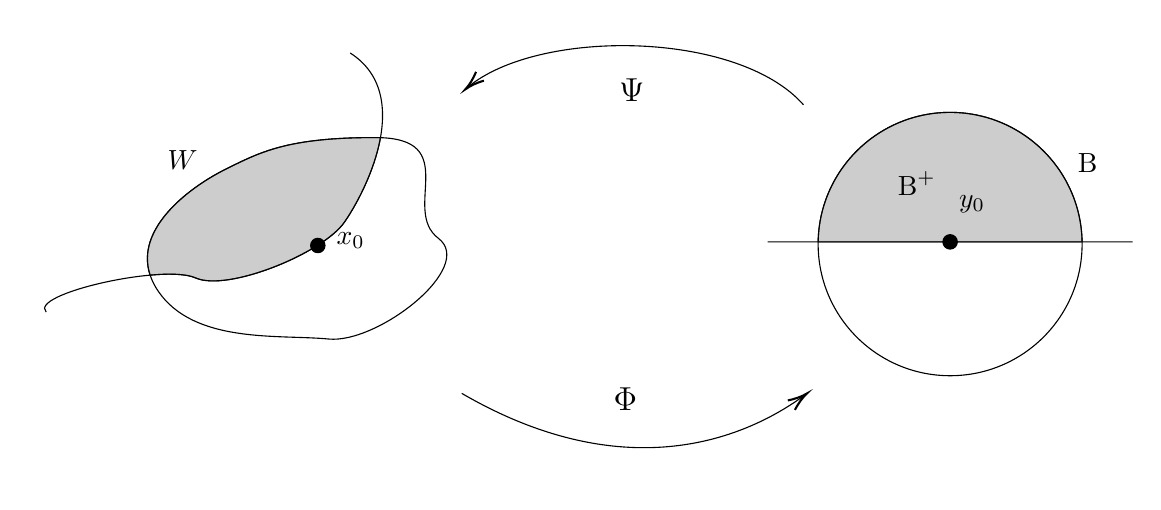
\begin{tikzpicture}[x=0.65pt,y=0.65pt,yscale=-1,xscale=1]
			%uncomment if require: \path (0,300); %set diagram left start at 0, and has height of 300
			
			%Shape: Ellipse [id:dp0023267519166336736] 
			\draw   (457.13,131.8) .. controls (457.13,91.37) and (489.98,58.6) .. (530.5,58.6) .. controls (571.02,58.6) and (603.87,91.37) .. (603.87,131.8) .. controls (603.87,172.23) and (571.02,205) .. (530.5,205) .. controls (489.98,205) and (457.13,172.23) .. (457.13,131.8) -- cycle ;
			%Shape: Polygon Curved [id:ds9277975115378949] 
			\draw   (127,90.6) .. controls (147,80.6) and (162,72.6) .. (211,72.6) .. controls (260,72.6) and (225,112.6) .. (246,128.6) .. controls (267,144.6) and (212.41,187.27) .. (185,184.6) .. controls (157.59,181.93) and (110,187.6) .. (90,157.6) .. controls (70,127.6) and (107,100.6) .. (127,90.6) -- cycle ;
			%Curve Lines [id:da9936244162893775] 
			\draw    (28,169.6) .. controls (18,159.6) and (93.25,142.66) .. (111,150.6) .. controls (128.75,158.54) and (181.67,136.96) .. (193.74,119.69) .. controls (205.81,102.42) and (233,48.6) .. (197,25.6) ;
			
			%Straight Lines [id:da09958792944365125] 
			\draw    (429,130.6) -- (632,130.58) ;
			
			%Curve Lines [id:da5907621652570023] 
			\draw    (259,214.8) .. controls (343.15,263.71) and (409.66,245.18) .. (449.79,215.7) ;
			\draw [shift={(451,214.8)}, rotate = 143.13] [color={rgb, 255:red, 0; green, 0; blue, 0 }  ][line width=0.75]    (10.93,-3.29) .. controls (6.95,-1.4) and (3.31,-0.3) .. (0,0) .. controls (3.31,0.3) and (6.95,1.4) .. (10.93,3.29)   ;
			%Curve Lines [id:da5283825799891098] 
			\draw    (449,54.4) .. controls (412.37,12.82) and (301.25,11.82) .. (262.16,44.79) ;
			\draw [shift={(261,45.8)}, rotate = 318.18] [color={rgb, 255:red, 0; green, 0; blue, 0 }  ][line width=0.75]    (10.93,-3.29) .. controls (6.95,-1.4) and (3.31,-0.3) .. (0,0) .. controls (3.31,0.3) and (6.95,1.4) .. (10.93,3.29)   ;
			%Shape: Path Data [id:dp48216478983696454] 
			\draw  [fill={rgb, 255:red, 155; green, 155; blue, 155 }  ,fill opacity=0.5 ] (211,72.6) .. controls (211.97,72.6) and (212.9,72.62) .. (213.81,72.65) .. controls (210.35,91.89) and (200.01,110.72) .. (193.74,119.69) .. controls (181.67,136.96) and (128.75,158.54) .. (111,150.6) .. controls (106.04,148.38) and (96.59,148.1) .. (85.76,149.08) .. controls (76.93,122.59) and (108.92,99.64) .. (127,90.6) .. controls (147,80.6) and (162,72.6) .. (211,72.6) -- cycle ;
			%Shape: Path Data [id:dp8186232193666636] 
			\draw  [fill={rgb, 255:red, 155; green, 155; blue, 155 }  ,fill opacity=0.5 ] (530.5,58.6) .. controls (570.62,58.6) and (603.21,90.72) .. (603.86,130.58) -- (457.14,130.6) .. controls (457.78,90.72) and (490.38,58.6) .. (530.5,58.6) -- cycle ;
			
			%Shape: Circle [id:dp6915413941378992] 
			\draw  [fill={rgb, 255:red, 0; green, 0; blue, 0 }  ,fill opacity=1 ] (175,132.6) .. controls (175,130.39) and (176.79,128.6) .. (179,128.6) .. controls (181.21,128.6) and (183,130.39) .. (183,132.6) .. controls (183,134.81) and (181.21,136.6) .. (179,136.6) .. controls (176.79,136.6) and (175,134.81) .. (175,132.6) -- cycle ;
			
			%Shape: Circle [id:dp5855646505789538] 
			\draw  [fill={rgb, 255:red, 0; green, 0; blue, 0 }  ,fill opacity=1 ] (526.5,130.59) .. controls (526.5,128.38) and (528.29,126.59) .. (530.5,126.59) .. controls (532.71,126.59) and (534.5,128.38) .. (534.5,130.59) .. controls (534.5,132.8) and (532.71,134.59) .. (530.5,134.59) .. controls (528.29,134.59) and (526.5,132.8) .. (526.5,130.59) -- cycle ;
			
			% Text Node
			\draw (534,103.4) node [anchor=north west][inner sep=0.75pt]    {$y_{0}$};
			% Text Node
			\draw (345,38.4) node [anchor=north west][inner sep=0.75pt]  [font=\large]  {$\Psi $};
			% Text Node
			\draw (342,210.4) node [anchor=north west][inner sep=0.75pt]  [font=\large]  {$\Phi $};
			% Text Node
			\draw (188,124) node [anchor=north west][inner sep=0.75pt]    {$x_{0}$};
			% Text Node
			\draw (94,78.4) node [anchor=north west][inner sep=0.75pt]    {$W$};
			% Text Node
			\draw (600,80) node [anchor=north west][inner sep=0.75pt]    {B};
			% Text Node
			\draw (500,90) node [anchor=north west][inner sep=0.75pt]    {$\textup{B}^+$};
		\end{tikzpicture}
	\end{center}
	
	Posto ora $W = \Psi(\textup{B})$, che non sarà una palla, ma comunque sarà un intorno aperto di $x_0$, convertendo quanto detto nelle variabili $x$, essendo lo jacobiano limitato, otteniamo un'estensione di $u$ a tutto $W$ con stima
	\[ \norm{\bar{u}}_{W^{1,p}(W)} \le C \norm{u}_{W^{1,p}(U)}. \]
	
	A questo punto, essendo $\partial U$ compatto, esisterà un numero finito di $x_j \in \partial U$ e di $W_j$ aperti tali che $u$ si estenda a $\bar{u}_j$ su $W_j$ e tali che 
	\[ \partial U \subseteq \bigcup_{j=1}^m W_j. \]
	Sia poi $W_0$ un aperto in $U$ tale che $\overline{W}_0 \subseteq U$ e 
	\[ U \subseteq \bigcup_{j=0}^m W_j \]
	e consideriamo una partizione dell'unità $(\xi_j)$ associata a questo ricoprimento. Posto $\bar{u}_0 = u$, definiamo
	\[ \bar{u} = \sum_{j=0}^{m}\xi_j \bar{u}_j. \]
	Potendo scegliere $\textup{B}$ di raggio arbitrariamente piccolo nei passaggi precedenti, si ha che $\bar{u}$ può sempre essere pensata con supporto in $V$. Inoltre, da un non proprio velocissimo calcolo, combinando le stime già ottenute, si vede che esiste $C > 0$ tale che
	\[ \norm{\bar{u}}_{W^{1,p}(\R^n)} \le C \norm{u}_{W^{1,p}(U)}. \]
	Da ciò possiamo concludere che se $u \in C^1(\overline{U})$, $Eu= \bar{u}$, con $E$ lineare per costruzione.
	
	Consideriamo ora il caso generale, ossia $u \in W^{1,p}(U)$. Per il Teorema \eqref{globapprbordo}, esiste $(u_m)$ in $C^\infty(\overline{U})$ tale che $u_m \to u$ in $W^{1,p}(U)$. Essendo convergente, allora $(u_m)$ è di Cauchy. Da fatto che 
	\[ \norm{Eu_m- Eu_l}_{W^{1,p}(\R^n)} = \norm{E(u_m- u_l)}_{W^{1,p}(\R^n)} \le C \norm{u_m - u_l}_{W^{1,p}(U)} \]
	otteniamo che  anche $(Eu_m)$ è una successione di Cauchy. Ma dal fatto che $W^{1,p}(\R^n)$ è di Banach risulta che $(Eu_m)$ è convergente. Risulta quindi ben definita l'estensione
	\[ Eu = \lim\limits_{m} Eu_m, \]
	infatti se si avesse anche $(v_m)$ in $C^\infty(\overline{U})$ tale che $v_m \to u$ in $W^{1,p}(U)$, risulterebbe
	\[ \norm{Eu_m- Ev_l}_{W^{1,p}(\R^n)} \le C \norm{u_m - v_l}_{W^{1,p}(U)} \]
	e dal fatto che 
	\[ \lim\limits_{m} u_m  = \lim\limits_{l} v_l = u\]
	si ha pertanto che 
	\[ \lim\limits_{l} Ev_l = Eu. \]
	Questo fornisce l'operatore richiesto. 
\end{proof}

\begin{definizione}
	Siano $1 \le p \le \infty$, $U$ limitato con $\partial U$ di classe $C^1$ e $V$ un aperto limitato tale che $\overline{U} \subseteq V$. Chiamiamo $Eu$\index[simboli]{$Eu$} un'\emph{estensione di $u$ a $\R^n$}\index[analitico]{estensione}.
\end{definizione}
\begin{osservazione}
	Se supponiamo inoltre che $\partial U$ sia di classe $C^2$, allora la stessa tecnica utilizzata nella dimostrazione del Teorema di estensione permette di ottenere un operatore $E: W^{2,p}(U) \to W^{2,p}(\R^n)$ lineare e continuo con le stesse proprietà viste nel Teorema di estensione. In particolare, esiste $C > 0$, dipendente solo da $U,V,n$ e $p$, tale che 
	\[ \norm{Eu}_{W^{2,p}(\R^n)}\le C\norm{u}_{W^{2,p}(U)}.  \] 
\end{osservazione}
\begin{osservazione}
	Se $k > 2$, è sempre possibile ottenere un Teorema di estensione. La dimostrazione è tuttavia più articolata e sfrutta delle tecniche di riflessione ad ordine superiore più complesse.
\end{osservazione}

\section{Tracce}
Se $u \in C(\overline{U})$, chiaramente ha senso parlare di valori su $\partial U$ per $u$. Invece, se $u \in W^{1,p}(U)$, in generale non è continua ed in più è definita solo quasi ovunque su $U$. Essendo $\partial U$ trascurabile, non c'è un modo diretto per parlare di valori al bordo. Introduciamo in questa sezione un operatore che gestisce queste situazioni.

\begin{teorema} \emph{\textbf{(di traccia)}}\index[analitico]{teorema!di traccia}
	Siano $1 \le p < \infty$ e $U$ limitato con $\partial U$ di classe $C^1$. Allora esiste un operatore lineare e continuo $T: W^{1,p}(U) \to L^p(\partial U)$ tale che
	\begin{enumerate}[$(a)$]
		\item $Tu = u |_{\partial U}$ ogniqualvolta $u \in W^{1,p}(U) \cap C(\overline{U})$;
		\item esiste $C >0$, dipendente solo da $p$ ed $U$, tale che
		\[ \norm{Tu}_{L^p(\partial U)} \le C \norm{u}_{W^{1,p}(U)}. \]
	\end{enumerate}
\end{teorema}
\begin{proof}
	Supponiamo inizialmente $u \in C^1(\overline{U})$. Fissiamo $x_0 \in \partial U$ e supponiamo anche che, in un intorno di $x_0$, $\partial U$ giaccia sul piano $x_n = 0$, ossia che esista $r > 0 $ tale che, detta $\textup{B} = \textup{B}(x_0,r)$,
	\begin{align*}
		\textup{B}^+ &:= \textup{B}(x_0,r) \cap \left\lbrace x_n \ge 0\right\rbrace \subseteq \overline{U}, \\
		\textup{B}^- &:= \textup{B}(x_0,r) \cap \left\lbrace x_n \le 0\right\rbrace \subseteq \R^n \setminus U.
	\end{align*}
	Sia anche $\hat{\textup{B}} = \textup{B}(x_0,\frac{r}{2}) $. Denotiamo con $\Gamma = \hat{\textup{B}} \cap \partial U$ e con $x' = \left( x_1,\dots, x_{n-1}\right) $, ossia $x = (x',x_n)$. Prendiamo $\zeta \in C^{\infty}_c(\textup{B})$ tale che $\zeta \ge 0$ in $\textup{B}$ e $\zeta = 1$ in $\hat{\textup{B}}$. Si ha, dalla Formula di Gauss--Green e dalla disuguaglianza di Young,
	\begin{align*}
		\int_\Gamma \abs{u}^pdx' &\le \int_{\left\lbrace x_n = 0\right\rbrace } \zeta \abs{u}^pdx' = \\
		& = - \int_{\textup{B}^+} D_{x_n}(\zeta \abs{u}^p)dx \le C \int_{\textup{B}^+} \left( \abs{u}^p + \abs{u}^{p-1}D_{x_n}u\right)  dx \le \\
		&\le C \int_{\textup{B}^+} \left( \abs{u}^p + \sum_{j=1}^{n} \abs{D_ju}^p\right)  dx \le C \norm{u}^p_{W^{1,p}(U)}.
	\end{align*}
	Consideriamo ora il caso in cui $\partial U$ non sia necessariamente piatto vicino ad $x_0$. Sia $\Phi$ il diffeomorfismo, con inversa $\Psi$, che appiattisce $\partial U$ in un intorno di $x_0$. Introduciamo le notazioni $y = \Phi(x)$, $x = \Psi(y)$ e $u'(y) = u(\Psi(y))$. Applicando la stima fatta nel caso precedente e cambiando variabili si ottiene la maggiorazione
	\[ 	\int_\Gamma \abs{u}^pdS \le C \norm{u}^p_{W^{1,p}(U)} \]
	dove ora $\Gamma$ è un qualche aperto di $\partial U$ contenente $x_0$.
	
	A questo punto, dalla compattezza di $\partial U$, segue che esisterà un numero finito di $x_j \in \partial U$ e di $\Gamma_j$ aperti in $\partial U$ tali che $\partial U = \bigcup_{j=1}^{m}\Gamma_j$ e per ogni $j=1,\dots,m$
	\[\norm{u}_{L^p(\Gamma_j)} \le C\norm{u}_{W^{1,p}(U)}. \]
	Detto quindi $Tu = u|_{\partial U}$, lineare per costruzione, si ha 
	\[ \norm{Tu}_{L^p(\partial U)} \le \sum_{j=1}^{m} \norm{Tu}_{L^p(\Gamma_j)} \le \tilde{C} \norm{u}_{W^{1,p}(U)} \]
	che fornisce la tesi in questo caso.
	
	Consideriamo ora il caso generale, ossia $u \in W^{1,p}(U)$. Per il Teorema \eqref{globapprbordo}, esiste $(u_m)$ in $C^\infty(\overline{U})$ tale che $u_m \to u$ in $W^{1,p}(U)$. Essendo convergente, allora $(u_m)$ è di Cauchy. Da fatto che 
	\[ \norm{Tu_m- Tu_l}_{L^{p}(\partial U)} = \norm{T(u_m- u_l)}_{L^{p}(\partial U)} \le C \norm{u_m - u_l}_{W^{1,p}(U)} \]
	otteniamo che  anche $(Tu_m)$ è una successione di Cauchy. Ma dal fatto che $L^{p}(\partial U)$ è di Banach risulta che $(Tu_m)$ è convergente. Risulta quindi ben definita l'estensione
	\[ Tu = \lim\limits_{m} Tu_m, \]
	infatti se si avesse anche $(v_m)$ in $C^\infty(\overline{U})$ tale che $v_m \to u$ in $W^{1,p}(U)$, risulterebbe
	\[ \norm{Tu_m- Tv_l}_{L^{p}(\partial U)} \le C \norm{u_m - v_l}_{W^{1,p}(U)} \]
	e dal fatto che 
	\[ \lim\limits_{m} u_m  = \lim\limits_{l} v_l = u\]
	si ha pertanto che 
	\[ \lim\limits_{l} Tv_l = Tu. \]
	Infine, se $u \in W^{1,p}(U)\cap C(\overline{U})$, allora $u_m \to u$ uniformemente e quindi dal fatto che il limite uniforme di applicazioni continue è continuo si ha
	\[ Tu = \lim_{m} Tu_m = \lim_{m} u_m|_{\partial U} = u|_{\partial U}\]
	e la dimostrazione è conclusa.
\end{proof}
\begin{definizione}
	Siano $1 \le p <\infty$ ed $U$ limitato con $\partial U$ di classe $C^1$. Chiamiamo $Tu$\index[simboli]{$Tu$} la \emph{traccia di $u$ su $\partial U$}\index[analitico]{traccia}.
\end{definizione}
Il seguente risultato permette di caratterizzare pienamente gli elementi di $W^{1,p}_0(U)$ come gli zeri dell'operatore di traccia. In questo senso risulta ora ragionevole l'espressione \emph{fare zero al bordo} per queste applicazioni.
\begin{teorema}
	Siano $1 \le p <\infty$, $U$ limitato con $\partial U$ di classe $C^1$ ed $u \in W^{1,p}(U)$. I seguenti fatti sono equivalenti:
	\begin{enumerate}[$(a)$]
		\item $u \in  W^{1,p}_0(U)$,
		\item $Tu = 0$ su $\partial U$.
	\end{enumerate}
\end{teorema}
\begin{proof}\hfill
	\par\noindent
	$(a) \Longrightarrow (b)$ Supponiamo $u \in W^{1,p}_0(U)$, allora esiste una successione $(u_m)$ in $C^\infty_c(U)$ tale che $u_m \to u$ in $W^{1,p}(U)$. Per continuità dell'operatore di traccia si ha che su $\partial U$ 
	\[ Tu = \lim\limits_{m} Tu_m = \lim\limits_{m} 0 = 0.  \]
	\par\noindent
	$(b) \Longrightarrow (a)$ Sia $u \in W^{1,p}(U)$ tale che $Tu = 0$ su $\partial U$. 
	
	Senza perdita di generalità possiamo limitarci al caso $u \in W^{1,p}(\R^n_{+})$ con $Tu = 0$ su $\partial\R^n_{+} = \R^{n-1} $.\footnote{Si tratta di appiattire il bordo di $U$, considerare, come nel teorema di estensione, una partizione dell'unità $(\xi_i)$ e scrivere $u = \sum_{i=0}^{\infty}u\xi_i$. A questo punto possiamo ragionare sui singoli termini della serie, che sono a supporto compatto e quindi definibili su tutto $\R^n_+$.}
	
	Dal fatto che $Tu = 0$ su $\R^{n-1} $, segue che esiste una successione $(u_m)$ in $C^1(\R^n_{+})$, tale che $u_m \to u$ in $W^{1,p}(\R^n_{+})$ e $Tu_m = u_m|_{\R^{n-1}} \to 0$ in $L^p(\R^{n-1})$.
	
	Indicando $x = (x,x_n)$, dove possiamo orientare gli assi in modo da avere $x_n \ge 0$, dal Teorema fondamentale del calcolo integrale segue
	\[ \abs{u_m(x',x_n)} \le \abs{u_m(x',0)}+ \int_{0}^{x_n} \abs*{D_{x_n}u_m(x',t)}dt \]
	da cui
	\[ \abs{u_m(x',x_n)}^p \le C\left(  \abs{u_m(x',0)}^p+ \left( \int_{0}^{x_n} \abs*{D_{x_n}u_m(x',t)}dt\right) ^p\right).  \]
	Integrando in $x'$, otteniamo
	\[ \int_{\R^{n-1}}\abs{u_m(x',x_n)}^p dx' \le C \left( \int_{\R^{n-1}} \abs{u_m(x',0)}^pdx'+ \int_{\R^{n-1}}\left( \int_{0}^{x_n} \abs*{Du_m(x',t)}dt\right) ^pdx'\right)  \]
	ma per la disuguaglianza di Holder,
	\[ \int_{0}^{x_n} \abs*{Du_m(x',t)}dt \le x_n^{\frac{p-1}{p}}\left( \int_{0}^{x_n}\abs*{Du_m(x',t)}^pdt\right)^{\frac{1}{p}},  \]
	perciò
	\[ 	\int_{\R^{n-1}}\abs{u_m(x',x_n)}^p dx' \le C \left( \int_{\R^{n-1}} \abs{u_m(x',0)}^pdx' + x_n^{p-1}\int_{\R^{n-1}} \int_{0}^{x_n}\abs*{Du_m(x',t)}^pdt dx'\right).  \]
	A questo punto, dal fatto che $u_m \to u$ in $W^{1,p}(\R^n_{+})$ e $Tu_m = u_m|_{\R^{n-1}} \to 0$ in $L^p(\R^{n-1})$, combinato con il Lemma di Fatou ed il Teorema di Fubini--Tonelli, risulta che per q.o. $x_n \ge 0$
	\begin{equation}\label{maggiorazionetraccia0}
		\int_{\R^{n-1}}\abs{u(x',x_n)}^p dx' \le C x_n^{p-1} \int_{0}^{x_n}\int_{\R^{n-1}}\abs*{Du(x',t)}^p dx'dt.
	\end{equation}
	Sia ora $\zeta \in C^\infty(\R^+)$ tale che $\zeta = 1$ in $[0,1]$, $\zeta = 0$ in $\R\setminus [0,2]$ e $0\le \zeta \le 1$. Consideriamo le successioni $(\zeta_m)$ e $(w_m)$ in $R^n_{+}$ tali che
	\[ \zeta_m(x) = \zeta(mx_n), \]
	\[ w_m(x) = u(x)(1-\zeta_m(x)). \]
	Chiaramente
	\[ D_{x_n}w_m(x) =  \left( 1-\zeta_m(x)\right)D_{x_n}u(x)  -mu \zeta'_m(x), \]
	\[ D_{x'}w_m(x) = \left( 1-\zeta_m(x)\right)D_{x'}u(x). \]
	Di conseguenza,
	\[ \int_{\R^n_+}\abs{Dw_n -Du}^p d\mathcal{L}^n \le C \int_{\R^n_+}\abs{\zeta_m}^p\abs{Du}^pd\mathcal{L}^n + Cm^p\int_{0}^{\frac{2}{m}}\int_{\R^{n-1}}\abs{u}^p dx'dt.  \]
	A questo punto, per \eqref{maggiorazionetraccia0},
	\begin{align*}
		Cm^p\int_{0}^{2m}\int_{\R^{n-1}}\abs{u}^p dx'dt &\le C m^p \int_{0}^{\frac{2}{m}}t^{p-1}dt \int_{0}^{\frac{2}{m}}\int_{\R^{n-1}}\abs{Du}^pdx'dt \le \\
		&\le C \int_{0}^{\frac{2}{m}}\int_{\R^{n-1}}\abs{Du}^pdx'dt
	\end{align*}
	e quindi dal Teorema della convergenza dominata si ha che $Dw_m \to Du$ in $L^{p}(\R^n_{+})$. Dal fatto che, chiaramente, $w_m \to u$ in $L^{p}(\R^n_{+})$ possiamo quindi affermare che $w_m \to u$ in $W^{1,p}(\R^n_{+})$. Dal fatto che $w_m = 0 $ se $0 < x_n < \frac{1}{m}$, segue che possiamo regolarizzare la successione $(w_m)$ producendo una successione $(u_m)$ in $C^\infty_c(\R^n_{+})$ tale che $u_m \to u$ in $W^{1,p}(\R^n_{+})$, ossia $u \in W^{1,p}_0(\R^n_{+})$.
\end{proof}
\section{Teoremi di immersione}
Se $u \in W^{1,p}(U)$, per definizione $u \in L^p(U)$. In questa sezione vediamo come il fatto che anche $D_ju \in L^p(U)$, fornisca un guadagno sulla sommabilità di $u$.

Iniziamo facendo un piccolo esperimento.
\begin{osservazione}
	Sia $1 \le p < n$. Supponiamo che esistano $C > 0$ e $q \in \left[ 1,\infty \right[ $ tali che per ogni $u \in C^\infty_c(\R^n)$ si abbia
	\[ \norm{u}_{L^q(\R^n)} \le C \norm{Du}_{L^p(\R^n)}. \]
	
	Sia $\lambda > 0$ e definiamo $u_\lambda(x) = u(\lambda x)$. Applicando la disuguaglianza a $u_\lambda$ otteniamo 
	\[ \frac{1}{\lambda^{\frac{n}{q}}}\norm{u}_{L^q(\R^n)} \le C \frac{\lambda}{\lambda^{\frac{n}{p}}}\norm{Du}_{L^p(\R^n)} \]
	da cui
	\[\norm{u}_{L^q(\R^n)} \le C \lambda^{1-\frac{n}{p}+\frac{n}{q}}\norm{Du}_{L^p(\R^n)}.  \]
	Se, per assurdo, $1-\frac{n}{p}+\frac{n}{q} \ne 0$ siamo di fronte a due casi:
	\begin{itemize}
		\item se $1-\frac{n}{p}+\frac{n}{q} > 0$, mandando $\lambda \to 0$, si ottiene una contraddizione,
		\item se $1-\frac{n}{p}+\frac{n}{q} < 0$, mandando $\lambda \to \infty$, si ottiene ancora una contraddizione.
	\end{itemize} 
	Perciò l'esponente deve essere necessariamente nullo, ossia $q = \frac{np}{n-p}$.
\end{osservazione}
La precedente osservazione motiva la seguente definizione.
\begin{definizione}
	Per ogni $p \in \left[ 1,\infty\right] $, poniamo 
	\[ p^* := \begin{cases}
		\infty & \textup{se }p=n, \\
		\frac{np}{n-p} & \textup{se } p < n.
	\end{cases} \]
	Diciamo che $p^*$ è l'esponente \emph{coniugato di Sobolev}\index[analitico]{coniugato di Sobolev}\index[simboli]{$p^*$} di $p$.
\end{definizione}
È evidente che $p^* > p$ e 
\[ \frac{1}{p^*} = \frac{1}{p} - \frac{1}{n}. \]
Vedremo più avanti il motivo per cui non abbiamo speso fatica cercando di estendere la definizione di esponente coniugato di Sobolev anche per $p>n$. In ogni caso, iniziamo studiando il caso $p < n$.
\begin{teorema}\emph{\textbf{(disuguaglianza di Gagliardo--Nirenberg--Sobolev)}}\label{GNS}\index[analitico]{disuguaglianza! di Gagliardo--Nirenberg--Sobolev}
	Sia $p \in \left[ 1, n\right[ $. Allora esiste $C > 0$, dipendente solo da $p$ e $n$, tale che per ogni $u \in C^1_c(\R^n)$ si abbia
	\[  \norm{u}_{L^{p^*}(\R^n)}\le C \norm{Du}_{L^p(\R^n)}. \]
\end{teorema}
\begin{proof}
	Consideriamo innanzitutto il caso $p = 1$. Allora $p^\ast = \frac{n}{n-1}$ e dal Teorema fondamentale del calcolo integrale, siccome $u(y) = 0$ per ogni $y \notin \textup{supt}(u)$,
	\[ u(x) = \int_{-\infty}^{x_i} D_{x_i}u(x_1,\dots,x_{i-1},y_i,x_{i+1},\dots,x_n)dy_i, \]
	da cui
	\[ \abs{u(x)} \le \int_{-\infty}^{+\infty} \abs{Du(x_1,\dots,x_{i-1},y_i,x_{i+1},\dots,x_n)}dy_i. \]
	Allora,
	\[ \abs{u(x)}^{\frac{n}{n-1}} \le \prod_{i=1}^{n}\left( \int_{-\infty}^{+\infty} \abs{Du(x_1,\dots,x_{i-1},y_i,x_{i+1},\dots,x_n)}dy_i\right) ^{\frac{1}{n-1}} \]
	per ogni $x \in \R^n$. Effettuiamo ora una prima integrazione rispetto ad $x_1$, 
	\begin{align*}
		\int_{-\infty}^{+\infty} \abs{u}^{\frac{n}{n-1}}dx_1 &\le \int_{-\infty}^{+\infty} \prod_{i=1}^{n}\left( \int_{-\infty}^{+\infty} \abs{Du(x_1,\dots,x_{i-1},y_i,x_{i+1},\dots,x_n)}dy_i\right) ^{\frac{1}{n-1}} dx_1 = \\
		&= \int_{-\infty}^{+\infty} \left( \int_{-\infty}^{+\infty} \abs{Du}dy_1\right) ^{\frac{1}{n-1}} \prod_{i=2}^{n}\left( \int_{-\infty}^{+\infty} \abs{Du}dy_i\right) ^{\frac{1}{n-1}} dx_1 = \\
		& = \left( \int_{-\infty}^{+\infty} \abs{Du}dy_1\right) ^{\frac{1}{n-1}} \int_{-\infty}^{+\infty} \prod_{i=2}^{n}\left( \int_{-\infty}^{+\infty} \abs{Du}dy_i\right) ^{\frac{1}{n-1}} dx_1
	\end{align*}
	e per la disuguaglianza di Holder generalizzata otteniamo 
	\[ \int_{-\infty}^{+\infty} \abs{u}^{\frac{n}{n-1}}dx_1 \le \left( \int_{-\infty}^{+\infty} \abs{Du}dy_1\right) ^{\frac{1}{n-1}} \left(\prod_{i=2}^{n}\int_{-\infty}^{+\infty}  \int_{-\infty}^{+\infty} \abs{Du}dy_idx_1\right) ^{\frac{1}{n-1}}. \]
	Procediamo ora con una integrazione rispetto ad $x_2$,
	\begin{align*}
		\int_{-\infty}^{+\infty}&\int_{-\infty}^{+\infty} \abs{u}^{\frac{n}{n-1}}dx_1 dx_2 \le \\
		&\le \int_{-\infty}^{+\infty}\left( \int_{-\infty}^{+\infty} \abs{Du}dy_1\right) ^{\frac{1}{n-1}} \left(\prod_{i=2}^{n}\int_{-\infty}^{+\infty}  \int_{-\infty}^{+\infty} \abs{Du}dy_idx_1\right) ^{\frac{1}{n-1}}dx_2,
	\end{align*}
	quindi
	\begin{align*}
		\int_{-\infty}^{+\infty}&\int_{-\infty}^{+\infty} \abs{u}^{\frac{n}{n-1}}dx_1 dx_2 \le \\
		&\le \left( \int_{-\infty}^{+\infty} \int_{-\infty}^{+\infty} \abs{Du}dx_1dy_2\right) ^{\frac{1}{n-1}} \\
		&\int_{-\infty}^{+\infty} \left( \int_{-\infty}^{+\infty}\abs{Du}dy_1\right)^{\frac{1}{n-1}}  \prod_{i=3}^{n} \left( \int_{-\infty}^{+\infty}\int_{-\infty}^{+\infty}\abs{Du}dx_1 dy_i\right) ^{\frac{1}{n-1}} dx_2
	\end{align*}
	ed applicando nuovamente la disuguaglianza di Holder generalizzata si ha
	\begin{align*}
		\int_{-\infty}^{+\infty}&\int_{-\infty}^{+\infty} \abs{u}^{\frac{n}{n-1}}dx_1 dx_2 \le \\
		&\le \left( \int_{-\infty}^{+\infty}\int_{-\infty}^{+\infty}\abs{Du}dx_1dy_2\right) ^{\frac{1}{n-1}}\left( \int_{-\infty}^{+\infty}\int_{-\infty}^{+\infty}\abs{Du}dy_1dx_2\right) ^{\frac{1}{n-1}} \\
		& \prod_{i=3}^{n} \left(\int_{-\infty}^{+\infty} \int_{-\infty}^{+\infty}\int_{-\infty}^{+\infty}\abs{Du}dx_1dx_2 dy_i\right) ^{\frac{1}{n-1}}
	\end{align*}
	dove i primi due integrali sono uguali per il Teorema di Fubini--Tonelli. A questo punto, procedendo ricorsivamente ed applicando il Teorema di Fubini--Tonelli si ottiene
	\[ 	\int_{\R^n}\abs{u}^{\frac{n}{n-1}}d\mathcal{L}^n \le \prod_{i=1}^n \left( \int_{\R^n} \abs{Du}d\mathcal{L}^n\right) ^{\frac{1}{n-1}} = \left( \int_{\R^n} \abs{Du}d\mathcal{L}^n\right) ^{\frac{n}{n-1}} \]
	ossia $\norm{u}_{\frac{n}{n-1}} \le \norm{Du}_1$. Consideriamo ora il caso $1 < p < n$. Dato $\gamma > 1$, applichiamo la stima precedente a $v = \abs{u}^\gamma$
	\[ \left(	\int_{\R^n}\abs{u}^{\frac{\gamma n}{n-1}}d\mathcal{L}^n\right) ^{\frac{n-1}{n}} \le \int_{\R^n} \gamma \abs{u}^{\gamma -1}\abs{Du}d\mathcal{L}^n \]
	ed utilizzando la disuguaglianza di Holder
	\[ \left(\int_{\R^n}\abs{u}^{\frac{\gamma n}{n-1}}d\mathcal{L}^n\right) ^{\frac{n-1}{n}} \le C \left( \int_{\R^n} \abs{u}^{\frac{(\gamma -1)p}{p-1}}d\mathcal{L}^n\right) ^{\frac{p-1}{p}} \left(\int_{\R^n} \abs{Du}^p d\mathcal{L}^n\right) ^{\frac{1}{p}}.  \]
	La posizione\footnote{It's a kind of magic!} $ \gamma = \frac{p(n-1)}{n-p} $ che corrisponde alla condizione
	\[ \frac{\gamma n}{n-1} = \left( \gamma -1\right) \frac{p}{p-1} \]
	fornisce 
	\[ \frac{\gamma n}{n-1} = p^{\ast} \]
	e 
	\[ \left(\int_{\R^n}\abs{u}^{p^{\ast}}d\mathcal{L}^n\right) ^{\frac{1}{p^{\ast}}} \le C \left(\int_{\R^n} \abs{Du}^p d\mathcal{L}^n\right) ^{\frac{1}{p}} \]
	che è la tesi.
\end{proof}
\begin{osservazione}
	L'ipotesi di supporto compatto nel Teorema \eqref{GNS} è necessaria: basti pensare alle funzioni costanti. Se per assurdo si potesse eliminare l'ipotesi, otterremmo $+\infty \le 0$. Comunque $C$ non dipende dall'ampiezza del supporto in quanto non dipende da $u$.
\end{osservazione}
\begin{teorema}\textbf{\emph{(di Sobolev)}}\label{thdiSobolev}\index[analitico]{teorema! di Sobolev}
	Siano $1 \le p < n$, $U$ limitato con $\partial U$ di classe $C^1$ e $u \in W^{1,p}(U)$. Allora $u \in L^{p^\ast}(U)$ ed esiste $C$, dipendente solo da $p,n$ ed $U$, tale che 
	\[ \norm{u}_{L^{p^\ast}(U)} \le C\norm{u}_{W^{1,p}(U)}. \]
\end{teorema}
\begin{proof}
	Innanzitutto per il Teorema di estensione, sia $\overline{u} = Eu \in W^{1,p}(\R^{n})$ tale che $\overline{u} = u$ q.o. in $U$, $\overline{u}$ è a supporto compatto in $\R^n$ e 
	\[ \norm{\overline{u}}_{W^{1,p}(\R^n)} \le C \norm{u}_{W^{1,p}(U)}. \]
	Siccome $\overline{u}$ è a supporto compatto, per il Teorema di locale approssimazione con funzione lisce, esiste $(u_h)$ in $C^\infty_c(\R^n)$ tale che $u_h \to \overline{u}$ in $W^{1,p}(\R^n)$. Ora, dalla Disuguaglianza di Sobolev, 
	\[ \norm{u_h - u_k}_{L^{p^\ast}(\R^n)} \le C\norm{Du_h - Du_k}_{L^p(\R^n)} \]
	allora $(u_h)$ è di Cauchy in $L^{p^\ast}(\R^n)$, per cui è convergente ad un certo $v$ in $L^{p^\ast}(\R^n)$. Per unicità del limite\footnote{Basta passare a delle sottosuccessioni per verificarlo esplicitamente.} si ha che $\overline{u}=v$ q.o. in $\R^n$. Ora, per il Teorema \eqref{GNS},
	\[ \norm{u_h}_{L^{p^\ast}(\R^n)} \le C \norm{Du_h}_{L^p(\R^n)} \]
	e se $h \to +\infty$
	\[ \norm{\overline{u}}_{L^{p^\ast}(\R^n)} \le C \norm{D\overline{u}}_{L^p(\R^n)} \le C\norm{\overline{u}}_{W^{1,p}(\R^n)}, \]
	ma 
	\[ \norm{\overline{u}}_{W^{1,p}(\R^n)} \le C \norm{u}_{W^{1,p}(U)}\]
	e sicuramente
	\[ \norm{u}_{L^{p^\ast}(U)} \le C \norm{\overline{u}}_{L^{p^\ast}(\R^n)} \]
	da cui 
	\[ \norm{u}_{L^{p^\ast}(U)} \le C\norm{u}_{W^{1,p}(U)}.\qedhere \]
\end{proof}

\begin{proposizione}
	Siano $1 \le p < n$, $U$ limitato con $\partial U$ di classe $C^1$ e $u \in W^{1,p}(U)$. Allora per ogni $q \in \left[ 1,p^\ast\right] $, $u \in L^{q}(U)$ ed esiste $C$, dipendente solo da $p,q,n$ ed $U$, tale che 
	\[ \norm{u}_{L^q(U)} \le C\norm{u}_{W^{1,p}(U)}. \]
\end{proposizione}
\begin{proof}
	Discende da Teorema \eqref{thdiSobolev} e dall'incapsulamento degli spazi di Lebesgue per $U$ limitato.
\end{proof}
Vediamo ora una disuguaglianza che, limitatamente alle $u \in W^{1,p}_0(U)$, estende al caso di un dominio limitato la disuguaglianza di Gagliardo--Nirenberg--Sobolev.
\begin{teorema}\textbf{\emph{(disuguaglianza di Poincaré)}}\index[analitico]{disuguaglianza! di Poincaré}\label{disPoincaré}
	Siano $1 \le p < +\infty$, $U$ limitato e $u \in W^{1,p}_0(U)$. Allora per ogni $q \in \left[ 1,p^\ast\right] $, $u \in L^{q}(U)$ ed esiste $C$, dipendente solo da $p,q,n$ ed $U$, tale che 
	\[ \norm{u}_{L^q(U)} \le C\norm{Du}_{L^p(U)}. \]
\end{teorema}
\begin{proof}
	Vediamo solo il caso $1 \le p < n$. Per definizione esiste $(u_m)$ in $C^\infty_c(U)$ tale che $u_m \to u$ in $W^{1,p}(U)$. Per il Teorema \eqref{GNS}, 
	\[ \norm{u_m}_{L^{p^\ast}(\R^n)} \le C \norm{Du_m}_{L^p(\R^n)} = C\norm{Du_m}_{L^p(U)} \]
	e analogamente $\norm{u_m}_{L^{p^\ast}(\R^n)} = \norm{u_m}_{L^{p^\ast}(U)}$, così che
	\begin{equation}\label{eqPoincaré}
		\norm{u_m}_{L^{p^\ast}(U)}\le C\norm{Du_m}_{L^p(U)}.
	\end{equation}
	Il secondo membro converge per definizione a $C\norm{Du}_{L^p(U)}$. Per quanto riguarda il primo membro è sufficiente osservare che esiste una sottosuccessione $(u_{m_k})$ convergente a $u$ q.o. in $U$, per cui, per il Lemma di Fatou,
	\[ \norm{u}_{L^{p^\ast}(U)} \le \underset{k}{\textup{lim inf }} \norm{u_{m_k}}_{L^{p^\ast}(U)} \]
	e, quindi, scrivendo la \eqref{eqPoincaré} per la sottosuccessione $(u_{m_k})$ e passando al lim inf si ha 
	\[ \norm{u}_{L^{p^\ast}(U)} \le C\norm{Du_m}_{L^p(U)}.\]
	Dall'incapsulamento degli spazi di Lebesgue per $U$ limitato segue la tesi.
\end{proof}
\begin{osservazione}
Vale la pena osservare che, limitatamente al caso $p<n$ e $q=p^\ast$, è possibile rimuovere le ipotesi di limitatezza su $U$. In particolare, in questo caso la costante $C$ dipende solo da $p$ ed $n$.
\end{osservazione}

\begin{osservazione}
	In $W^{1,p}_0(U)$ la norma $ \norm{Du}_{L^p(U)} $ è equivalente alla norma $\norm{u}_{W^{1,p}(U)}$. Infatti già sappiamo che
	\[ \norm{Du}_{L^p(U)} \le c_1 \norm{u}_{W^{1,p}(U)} . \]
	Per la Disuguaglianza di Poincaré otteniamo proprio l'altra stima. In particolare $H^{1}_0(U)$ munito della norma del gradiente è uno spazio di Hilbert.
\end{osservazione}

\begin{proposizione}\textbf{\emph{(disuguaglianza di Poincaré duale)}}\index[analitico]{disuguaglianza! di Poincaré!duale}\label{disPoincaréduale}
	Siano $\frac{n}{n-1} < q \le +\infty$ e $u \in L^{\frac{nq}{n+q}}(U)$. Allora , $u \in W^{-1,q}(U)$ ed esiste $C$, dipendente solo da $n$ e $q$, tale che 
	\[ \norm{u}_{W^{-1,q}(U)} \le C\norm{u}_{L^{\frac{nq}{n+q}}(U)}, \]
	dove si pone $\frac{nq}{n+q} = n$ ogniqualvolta $q=+\infty$.
\end{proposizione}
\begin{proof}
	Data $u \in  L^{\frac{nq}{n+q}}(U)$, consideriamo $T_u: W^{1,q'}_0(U) \to \R$ tale che 
	\[ \braket{T_u, v} = \int_U uvd\mathcal{L}^n. \]
	A meno di identificare $u$ e $T_u$, per la disuguaglianza di Holder\footnote{Siccome $\left( \frac{nq}{n+q}\right)' =(q')^\ast$.},
	\[ \abs{\braket{u,v}} \le \int_U \abs{u} \abs{v} d\mathcal{L}^n \le \norm{u}_{L^{\frac{nq}{n+q}}(U)} \norm{v}_{L^{(q')^\ast}(U)}\]
	e, per la disuguaglianza di Poincaré,
	\[ \abs{\braket{u,v}} \le  \norm{u}_{L^{\frac{nq}{n+q}}(U)} C \norm{v}_{W^{1,q'}_0(U)}, \]
	da cui la tesi.
\end{proof}
\begin{osservazione}
	La disuguaglianza di Poincaré duale può essere dimostrata anche semplicemente osservando il seguente fatto generale: consideriamo $X,Y$ due spazi di Banach su $\R$ tali che $X\subseteq Y$. Se l'immersione $X \hookrightarrow Y$ è continua, allora l'immersione $Y' \hookrightarrow X'$ è continua.\footnote{Questo deriva dal fatto che, essendo $X \subseteq Y$, a meno di identificare $\varphi \in Y'$ con $\varphi|_X$, l'immersione è ben definita e lineare. La continuità segue osservando che per ogni $\varphi \in Y'$
		\[ \norm{\varphi}_{X'} = \underset{\underset{z \in X}{\abs{z}\le 1}}{\sup}\; \abs{\braket{\varphi,x}} \le  \underset{\underset{z \in Y}{\abs{z}\le 1}}{\sup}\; \abs{\braket{\varphi,x}} = \norm{\varphi}_{Y'}.\]}
	
	Dalla disuguaglianza di Poincaré, sappiamo che l'immersione $W^{1,q'}_0(U)  \hookrightarrow L^{(q')^\ast}(U)$ è continua, quindi lo è anche l'immersione $(L^{(q')^\ast}(U))' \hookrightarrow W^{-1,q}(U)$. In altre parole, l'immersione $(L^{((q')^\ast)'}(U)) \hookrightarrow W^{-1,q}(U)$ è continua. A questo punto è sufficiente osservare che $((q')^\ast)' =\frac{nq}{n+q}$.
	
\end{osservazione}



\begin{osservazione}\label{probleman=p}
	Dal fatto che 
	\[ \lim\limits_{n \to p} \frac{np}{n-p} = +\infty, \]
	parrebbe ragionevole aspettarsi che se $u \in W^{1,n}(U)$, allora $u \in L^\infty(U)$. Tuttavia per $n > 1$ ciò è falso.
\end{osservazione}

Vediamo un controesempio che giustifica l'Osservazione \eqref{probleman=p}.
\begin{esempio}\footnote{Con leggere varianti si può fare anche in $\R^n$.}
	Sia $U = \textup{B}(0,1)$ in $\R^2$ e 
	\[ u(x) = \ln \left( \ln \left( 1 + \frac{1}{\abs{x}}\right)\right)  . \]
	Chiaramente $u \notin L^\infty(U)$. Mostriamo che $u \in W^{1,2}(U)$. Passando alle coordinate polari si vede subito che
	\[ \int_{U} \ln^2 \left( \ln \left( 1 + \frac{1}{\abs{x}}\right)\right)d\mathcal{L}^2(x) \sim \int_{0}^{1} \ln^2 \left( \ln \left( 1 + \frac{1}{\rho}\right)\right)\rho d\rho.  \]
	Ora, posto $y =\ln \left( 1 + \frac{1}{\rho}\right)$,
	\[ \int_{0}^{1} \ln^2 \left( \ln \left( 1 + \frac{1}{\rho}\right)\right)\rho d\rho \sim \int_{\ln 2}^{+\infty} \dfrac{e^y \ln^2 y}{(e^y-1)^3} dy \sim \int_{\ln 2}^{+\infty} \frac{\ln^2 y}{e^{2y}} dy. \]
	Ricordando che $\ln y \le y-1$ per ogni $y > 0$, 
	\[ \int_{\ln 2}^{+\infty} \frac{\ln^2 y}{e^{2y}} dy \le  \int_{\ln 2}^{+\infty} \frac{(y-1)^2}{e^{2y}} dy  \sim \int_{\ln 2}^{+\infty} \frac{y^2}{e^{2y}} dy. \]
	Se effettuiamo il cambio di variabile $y = \ln k$, otteniamo 
	\[ \int_{\ln 2}^{+\infty} \frac{y^2}{e^{2y}} dy = \int_{2}^{+\infty} \frac{1}{k^3\abs{\ln k}^{-2}}dk < +\infty \]
	da cui $u \in L^2(U)$. Invece, sempre utilizzando le coordinate polari osserviamo che
	\[ \int_{U} \abs{Du(x)}^2d\mathcal{L}^2(x) \sim \int_{0}^{1} \dfrac{1}{\rho(\rho + 1)^2\ln^2(1+\frac{1}{\rho})} d\rho \sim \int_{0}^{1} \frac{1}{\rho \ln^2(1+\frac{1}{\rho})} d\rho. \]
	Ora, posto $y =\ln \left( 1 + \frac{1}{\rho}\right)$,
	\[ \int_{0}^{1} \frac{1}{\rho \ln^2(1+\frac{1}{\rho})} d\rho \sim \int_{\ln 2}^{+\infty} \frac{1}{y^2} dy < +\infty \]
	da cui anche $Du \in L^2(U)$.  
\end{esempio}

Il caso $p=n$ è gestito dalla \emph{Disuguaglianza di Trudinger--Moser}, che non trattiamo nei dettagli. Passiamo quindi al caso $p > n$.
\begin{notazione}\index[simboli]{$\norm{u}_{C(\overline{U})}$}\index[simboli]{$\left[ u\right] _{C^{0,\gamma}(\overline{U})}$}\index[simboli]{$\norm{u}_{C(\overline{U})}$}\index[simboli]{$ \norm{u}_{C^{0,\gamma}(\overline{U})}$}
	Se $u \in C_b(U)$ e $\gamma \in \left] 0,1\right] $, indichiamo con
	\[ \left[ u\right] _{C^{0,\gamma}(\overline{U})} = \underset{\underset{x\ne y}{x, y \in U}}{\textup{sup}}\frac{\abs{u(x)-u(y)}}{\abs{x-y}^\gamma} \]
	e
	\[ \norm{u}_{C^{0,\gamma}(\overline{U})} = \norm{u}_{\infty} + \left[ u\right] _{C^{0,\gamma}(\overline{U})}.\]
\end{notazione}
\begin{definizione}
	Sia $\gamma \in \left] 0,1\right] $ e $k\ge 0$. Chiamiamo \emph{spazio di Holder}\index[analitico]{spazio! di Holder}, denotato con $C^{k,\gamma}(\overline{U})$\index[simboli]{$C^{k,\gamma}(\overline{U})$}, l'insieme delle $u \in C^k(\overline{U})$ tali che 
	\[ \norm{u}_{C^{k,\gamma}(\overline{U})} = \sum_{\abs{\alpha}\le k}\norm{D^\alpha u}_{\infty} + \sum_{\abs{\alpha}\le k} \left[ D^\alpha u\right] _{C^{0,\gamma}(\overline{U})} < +\infty.\]
\end{definizione}
\begin{proposizione}
	Sia $\gamma \in \left] 0,1\right] $ e $k\ge 0$. Allora $\norm{\ }_{C^{k,\gamma}(\overline{U})}$ è una norma su  $C^{k,\gamma}(\overline{U})$. Inoltre $\left(C^{k,\gamma}(\overline{U}),\norm{\ }_{C^{k,\gamma}(\overline{U})}\right)$ è uno spazio di Banach su $\R$.
\end{proposizione}
\begin{proof}
	Omettiamo la dimostrazione.
\end{proof}

Non è invece una norma $ \left[\ \right] _{C^{0,\gamma}(\overline{U})}$ in quanto nulla su tutte le funzioni costanti.

\begin{teorema}\textbf{\emph{(disuguaglianza di Morrey)}}\index[analitico]{disuguaglianza! di Morrey}
	Siano $n < p \le \infty$ e $\gamma = 1 - \frac{n}{p}$. Allora esiste $C$, dipendente solo da $p$ e $n$, tale che per ogni $u \in C^1(\R^n)$ si abbia
	\[ \norm{u}_{C^{0,\gamma}(\R^n)} \le C \norm{u}_{W^{1,p}(\R^n)}. \]
	\begin{proof}
		Limitiamo la dimostrazione al caso $p \ne \infty$. Sia $x \in \R^n$ ed $r >0$. Mostriamo che esiste $C$, dipendente solo da $n$ tale che
		\[ \fint_{\textup{B}(x,r)} \abs{u(y) - u(x)}d\mathcal{L}^n(y) \le C \int_{\textup{B}(x,r)} \frac{\abs{Du(y)}}{\abs{y-x}^{n-1}}d\mathcal{L}^n(y). \]
		Siano $w \in \partial \textup{B}(0,1)$ e $s \in \left] 0,r\right[ $. Chiaramente $\abs{w}=1$ e $x + sw \in \partial \textup{B}(x,s)$. Inoltre, per il Teorema fondamentale del calcolo integrale, 
		\[ \abs{u(x+sw) - u(x)} = \abs*{\int_{0}^{s}\frac{d}{dt}u(x+tw)dt} = \abs*{\int_{0}^{s}Du(x+tw) \cdot w dt} \le \int_{0}^{s} \abs*{Du(x+tw)}dt.  \]
		Integriamo ora rispetto a $w$, ottenendo
		\[ \int_{\partial\textup{B}(0,1)} \abs{u(x+sw) - u(x)} d\mathcal{H}^{n-1}(w) \le \int_{0}^{s} \int_{\partial\textup{B}(0,1)} \abs*{Du(x+tw)} d\mathcal{H}^{n-1}(w) dt. \]
		Consideriamo l'integrale
		\[ \int_{\textup{B}(x,s)} \frac{\abs{Du(y)}}{\abs{x-y}^{n-1}}d\mathcal{L}^n(y) \]
		ed applichiamogli il cambio di variabile $\varphi: \left] 0,s\right[ \times \partial \textup{B}(0,1) \to \textup{B}(x,s)$ tale che $y = \varphi(t,w) = x+tw$ ottenendo 
		\[ \int_{\textup{B}(x,s)} \frac{\abs{Du(y)}}{\abs{x-y}^{n-1}}d\mathcal{L}^n(y) =  \int_{0}^{s} \int_{\partial\textup{B}(0,1)} \abs*{Du(x+tw)} \frac{t^{n-1}}{t^{n-1}} d\mathcal{H}^{n-1}(w) dt.\]
		Pertanto,
		\begin{align*}
		\int_{\partial\textup{B}(0,1)} \abs{u(x+sw) - u(x)} d\mathcal{H}^{n-1}(w) &\le \int_{\textup{B}(x,s)} \frac{\abs{Du(y)}}{\abs{x-y}^{n-1}}d\mathcal{L}^n(y) \le \\
		&\le \int_{\textup{B}(x,r)} \frac{\abs{Du(y)}}{\abs{x-y}^{n-1}}d\mathcal{L}^n(y).
		\end{align*}
		Se ora moltiplichiamo ambo i membri per $s^{n-1}$ ed integriamo rispetto ad $s$ otteniamo 
		\[ 	\int_{0}^{r} s^{n-1} \int_{\partial\textup{B}(0,1)} \abs{u(x+sw) - u(x)} d\mathcal{H}^{n-1}(w) ds  \le \int_{0}^{r} s^{n-1} \int_{\textup{B}(x,r)} \frac{\abs{Du(y)}}{\abs{x-y}^{n-1}}d\mathcal{L}^n(y) ds \]
		ossia
		\[ \int_{\textup{B}(x,r)} \abs{u(y) - u(x)} d\mathcal{L}^{n}(y) \le \frac{r^n}{n} \int_{\textup{B}(x,r)} \frac{\abs{Du(y)}}{\abs{x-y}^{n-1}}d\mathcal{L}^n(y).  \]
		Dividendo ambo i membri per la misura di $\textup{B}(x,r)$ otteniamo proprio
		\[ \fint_{\textup{B}(x,r)} \abs{u(y) - u(x)}d\mathcal{L}^n(y) \le C \int_{\textup{B}(x,r)} \frac{\abs{Du(y)}}{\abs{y-x}^{n-1}}d\mathcal{L}^n(y).\footnote{A voler essere precisi, fino ad ora non abbiamo usato nessuna delle ipotesi del Teorema.} \]
		
		Mostriamo ora che 
		\[ \int_{\textup{B}(x,r)} \dfrac{1}{\abs{x-y}^{(n-1)\frac{p}{p-1}}}d\mathcal{L}^n(y) = C r^{\frac{p-n}{p-1}} < +\infty. \]
		Per fare ciò effettuiamo prima di tutto il cambio di variabile $z = x-y$,
		\[ \int_{\textup{B}(x,r)} \dfrac{1}{\abs{x-y}^{(n-1)\frac{p}{p-1}}}d\mathcal{L}^n(y) = \int_{\textup{B}(0,r)} \dfrac{1}{\abs{z}^{(n-1)\frac{p}{p-1}}}d\mathcal{L}^n(z)\]
		ed utilizzando poi le coordinate ipersferiche, ricordando che $n<p$,
		\[ \int_{\textup{B}(0,r)} \dfrac{1}{\abs{z}^{(n-1)\frac{p}{p-1}}}d\mathcal{L}^n(z) = C\int_{0}^{r} \rho^{\frac{1-n}{p-1}}d\rho = Cr^{\frac{p-n}{p-1}} < +\infty.  \]
		
		A questo punto, dato $x \in \R^n$ e $y \in \textup{B}(x,1)$,
		\[ \abs{u(x)} \le \abs{u(x) - u(y)} + \abs{u(y)} \]
		e quindi, integrando in media rispetto a $y$,
		\[ \abs{u(x)} \le \fint_{\textup{B}(x,1)}\abs{u(x) - u(y)} d\mathcal{L}^n(y) +  \fint_{\textup{B}(x,1)}\abs{u(y)} d\mathcal{L}^n(y)\]
		e, se nel primo integrale applichiamo la stima ricavata sopra e nel secondo la disuguaglianza di Holder otteniamo 
		\[ \abs{u(x)} \le C\int_{\textup{B}(x,1)} \frac{\abs{Du(y)}}{\abs{y-x}^{n-1}}d\mathcal{L}^n(y) + C\norm{u}_{L^{p}(\textup{B}(x,1))}. \]
		Se applichiamo la disuguaglianza di Holder al primo integrale possiamo scrivere
		\[ \int_{\textup{B}(x,1)} \frac{\abs{Du(y)}}{\abs{y-x}^{n-1}}d\mathcal{L}^n(y) \le \left( \int_{\textup{B}(x,1)} \abs{Du}^pd\mathcal{L}^n\right) ^{\frac{1}{p}}\left( \int_{\textup{B}(x,1)} \dfrac{1}{\abs{x-y}^{(n-1)\frac{p}{p-1}}} d\mathcal{L}^n(y) \right)^{\frac{p-1}{p}}.\]
		Allora possiamo scrivere
		\[ \abs{u(x)} \le C\norm{u}_{W^{1,p}(\R^n)} \]
		e dall'arbitrarietà di $x$, possiamo passare al $\textup{sup}$ ottenendo
		\begin{equation}\label{stimanormainfty}
			\norm{u}_{\infty} \le C\norm{u}_{W^{1,p}(\R^n)}. 
		\end{equation}
		\indent Siano ora $x,y \in \R^n$ ed indichiamo con $r = \abs{x-y}$ e con $W = \textup{B}(x,r) \cap \textup{B}(y,r)$. Se $w \in W$,
		\[ \abs{u(x)-u(y)} \le \abs{u(x)-u(w)} + \abs{u(y)-u(w)}\]
		e quindi procedendo con un'integrazione mediata rispetto a $w$
		\begin{align*}
			\abs{u(x)-u(y)} &\le \fint_{W}\abs{u(x)-u(w)}d\mathcal{L}^n(w) + \fint_{W}\abs{u(y)-u(w)}d\mathcal{L}^n(w) \le \\
			& \le \fint_{\textup{B}(x,r)}\abs{u(x)-u(w)}d\mathcal{L}^n(w) + \fint_{\textup{B}(y,r)}\abs{u(y)-u(w)}d\mathcal{L}^n(w).
		\end{align*}
		Siccome
		\[\fint_{\textup{B}(x,r)}\abs{u(x)-u(w)}d\mathcal{L}^n(w) \le C\int_{\textup{B}(x,r)} \frac{\abs{Du(y)}}{\abs{y-x}^{n-1}}d\mathcal{L}^n(y)   \]
		e applicando la disuguaglianza di Holder
		\begin{align*}
			\int_{\textup{B}(x,r)} \frac{\abs{Du(y)}}{\abs{y-x}^{n-1}}d\mathcal{L}^n(y) &\le C \left( \int_{\textup{B}(x,r)} \abs{Du}^pd\mathcal{L}^n\right) ^{\frac{1}{p}}\left( \int_{\textup{B}(x,r)} \dfrac{1}{\abs{x-y}^{(n-1)\frac{p}{p-1}}} d\mathcal{L}^n(y) \right)^{\frac{p-1}{p}} \le \\
			&\le C r^{1-\frac{n}{p}}\norm{Du}_{L^p(\R^n)}.
		\end{align*}
		Analogamente vale una stima simile per il secondo addendo, da cui
		\[ \abs{u(x)-u(y)} \le  C r^{1-\frac{n}{p}}\norm{Du}_{L^p(\R^n)} = C \abs{x-y}^{1-\frac{n}{p}}\norm{Du}_{L^p(\R^n)}\]
		e, per l'arbitrarietà di $x,y$,
		\begin{equation}\label{stimaseminormaholder}
			\left[ u\right] _{C^{0,\gamma}(\R^n)} \le C\norm{Du}_{L^p(\R^n)}.
		\end{equation}
		La tesi segue combinando \eqref{stimanormainfty} e \eqref{stimaseminormaholder}.
	\end{proof}
\end{teorema}
\begin{teorema}\textbf{\emph{(di Morrey)}}\index[analitico]{teorema! di Morrey}
	Siano $n < p \le \infty$, $\gamma = 1 - \frac{n}{p}$, $U$ limitato con $\partial U$ di classe $C^1$ e $u \in W^{1,p}(U)$. Allora esiste $C$, dipendente solo da $p,n$ e $U$, e un rappresentante della classe di equivalenza $u$, indicato con $u^\ast$, tale che $u^\ast \in C^{0,\gamma}(\overline{U})$
	\[ \norm{u^\ast}_{ C^{0,\gamma}(\overline{U})} \le C \norm{u}_{W^{1,p}(U)}.\]
\end{teorema}
\begin{proof}
	Innanzitutto per il Teorema di estensione, sia $\overline{u} = Eu \in W^{1,p}(\R^{n})$ tale che $\overline{u} = u$ q.o. in $U$, $\overline{u}$ è a supporto compatto in $\R^n$ e 
	\[ \norm{\overline{u}}_{W^{1,p}(\R^n)} \le C \norm{u}_{W^{1,p}(U)}. \]
	Dal fatto che $\overline{u}$ è a supporto compatto, esiste $(u_h)$ in $C^\infty_c(\R^n)$ tale che $u_h \to \overline{u}$ in $W^{1,p}(\R^n)$. Ora, dalla Disuguaglianza di Morrey, 
	\[ \norm{u_h - u_k}_{C^{0,\gamma}(\R^n)} \le C\norm{u_h - u_k}_{W^{1,p}(\R^n)} \]
	allora $(u_h)$ è di Cauchy in $C^{0,\gamma}(\R^n)$, per cui è convergente ad un certo $u^\ast$ in $C^{0,\gamma}(\R^n)$. Per unicità del limite puntuale si ha che $u=u^\ast$  q.o. in $U$.  Sempre per la Disuguaglianza di Morrey,
	\[ \norm{u_h}_{C^{0,\gamma}(\overline{U})} \le \norm{u_h}_{C^{0,\gamma}(\R^n)} \le C \norm{u_h}_{W^{1,p}(\R^n)}\]
	e se $h \to +\infty$
	\[ \norm{u^\ast}_{C^{0,\gamma}(\overline{U})} \le C \norm{\overline{u}}_{W^{1,p}(\R^n)}, \]
	da cui 
	\[ \norm{u^\ast}_{ C^{0,\gamma}(\overline{U})} \le C \norm{u}_{W^{1,p}(U)}.\qedhere\]
\end{proof}
Ricapitolando, se $U$ limitato con $\partial U$ di classe $C^1$, le seguenti immersioni sono continue:
\begin{description}
	\item[\textbf{Sobolev} ($\mathbf{1\le p< n}$)] $W^{1,p}(U) \hookrightarrow L^{q}(U)$ per ogni $1 \le q \le p^\ast$,
	\item[\textbf{Trudinger--Moser} ($\mathbf{p=n}$)] $W^{1,n}(U) \hookrightarrow L^{q}(U)$ per ogni $1 \le q < \infty$,
	\item[\textbf{Morrey} ($\mathbf{p > n}$)] $W^{1,p}(U) \hookrightarrow C^{0,1 - \frac{n}{p}}(\overline{U})$, quindi, in particolare, $W^{1,p}(U) \hookrightarrow L^{q}(U)$ per ogni $1 \le q \le \infty$.
\end{description}
In altre parole, all'aumentare di $p$ rispetto ad $n$ si ha un guadagno sempre maggiore sulla regolarità.

Vediamo alcune interessanti conseguenze nel caso $p>n$.
\begin{osservazione}
	In $\R$, se $U$ limitato con $\partial U$ di classe $C^1$, ogni $u \in H^1(U)$ ammette un rappresentante continuo.
\end{osservazione}

\begin{proposizione}
	Siano $U$ limitato con $\partial U$ di classe $C^1$ ed $u : U \to \R$. I seguenti fatti sono equivalenti:
	\begin{enumerate}[$(a)$]
		\item $u$ è lipschitziana,
		\item $u \in W^{1,\infty}(U)$.
	\end{enumerate}
	
	\begin{proof} Supponiamo $U = \R^n$ ed $u$ a supporto compatto in U. Il caso generale segue dal Teorema di estensione.
		\par\noindent
		$(b) \Longrightarrow (a)$ Se $u \in W^{1,\infty}(\R^n)$, allora $u^\varepsilon = \varrho_\varepsilon \ast u$ è tale che $u^\varepsilon \to u$ uniformemente per $\varepsilon \to 0$, in quanto esiste un rappresentante holderiano, quindi continuo, e 
		\[ \norm{Du^\varepsilon}_{L^\infty(\R^n)} \le \norm{Du}_{L^\infty(\R^n)}. \]
		Dati $x,y \in \R^n$ tali che $x \ne y$, per il Teorema fondamentale del calcolo integrale,
		\[\abs*{u^\varepsilon(x) - u^\varepsilon(y)} \le \int_{0}^{1} \abs*{Du^\varepsilon(tx + (1-t)y)}dt \abs{x-y} \le \norm{Du^\varepsilon}_{L^\infty(\R^n)} \abs{x-y} \]
		da cui 
		\[ \abs*{u^\varepsilon(x) - u^\varepsilon(y)} \le \norm{Du}_{L^\infty(\R^n)}\abs{x-y} \]
		e, per $\varepsilon \to 0$, dal fatto che il limite $u^\varepsilon \to u$ è uniforme, segue la lipschitzianità di $u$.
		\par\noindent
		$(a) \Longrightarrow (b)$ Supponiamo $u$ lipschitziana. Allora esiste $C>0$ tale che per ogni $x,y \in \R^n$
		\[ \abs{u(x) -u(y)}\le C\abs{x-y}. \]
		Consideriamo $(h_k)$ tale che $h_k \to 0$. Allora
		\[ \abs{u(x-h_ke_j) -u(x)}\le Ch_k \]
		da cui 
		\[ D^{-h_k}_ju(x) \le C \]
		e quindi $\norm{ D^{-h_k}_ju}_\infty \le C$ ossia $(D^{-h_k}_ju)$ limitata in $L^\infty(\R^n)$. Per l'Osservazione \eqref{convergenzadeboleLp}, esiste $w \in L^\infty$ tale che, a meno di sottosuccessioni, per ogni $\varphi \in L^1(\R^n)$ si abbia
		\[ \int D^{-h_k}_j u \varphi d\mathcal{L}^n \to \int w \varphi d\mathcal{L}^n \]
		e quindi in particolare per ogni $\varphi \in C^\infty_c(\R^n)$. Ma per \eqref{integrazioneperpartirapportoincrementale}, 
		\[ \int D_j^{-h_k}u\varphi d\mathcal{L}^n = -\int u D^{h_k}_j\varphi d\mathcal{L}^n. \]
		Allora per il Teorema della convergenza dominata, per ogni $\varphi \in C^\infty_c(\R^n)$
		\[ \int uD_j\varphi d\mathcal{L}^n = -\int w \varphi d\mathcal{L}^n \]
		da cui $D_j u = w \in L^\infty(\R^n)$, ossia $u \in W^{1,\infty}(\R^n)$.
	\end{proof}
\end{proposizione}
\begin{osservazione}
	In modo analogo $u \in W^{1,\infty}_{loc}(U)$ se e solo se $u$ è localmente lipschitziana in $U$. Inoltre, si può dimostrare che dati $U$ un aperto qualunque e $p \in \left] n,\infty\right[ $, se $u \in W^{1,p}(U)$ allora $u \in C^{0,1-\frac{n}{p}}(U)$.
\end{osservazione}
\begin{teorema}
	Sia $n < p \le \infty.$ Se $u \in W^{1,p}_{loc}(U)$ allora $u$ è differenziabile \emph{q.o.} in $U$. 
	
	In particolare, il gradiente di $u$ è uguale al gradiente debole di $u$ \emph{q.o.} in $U$.
	\begin{proof} Consideriamo dapprima il caso $p\ne \infty.$ Innanzitutto, fissati $x,y \in U$ e posto $r=\abs{x-y}$, per ogni $v \in C^1(\textup{B}(x,2r))$, in modo analogo a quanto fatto per dimostrare la disuguaglianza di Morrey, si ha che
		\[ \abs{v(y)-v(x)} \le C r^{1-\frac{n}{p}}\left( \int_{\textup{B}(x,2r)}\abs{Dv}^pd\mathcal{L}^n\right) ^{\frac{1}{p}}.\]
		La precedente relazione, mediante approssimazione, vale poi per ogni $v \in W^{1,p}(\textup{B}(x,2r))$, identificata con il suo rappresentante holderiano, quindi continuo. Sia ora $u \in W^{1,p}_{loc}(U)$, identificata con il suo rappresentante continuo. Per una variante del Teorema sui punti di Lebesgue, per q.o. $x \in U$
		\[ \lim\limits_{r \to 0} \fint_{\textup{B}(x,2r)} \abs{Du(x)-Du(y)}^pd\mathcal{L}^n(y) = 0. \]
		Scelta $v(y) = u(y)-u(x)-Du(x)\cdot(y-x)$, osservando che $v(x) = 0$,
		\[ \abs{u(y)-u(x)-Du(x)\cdot(y-x)} = \abs{v(y)-v(x)} \le Cr^{1-\frac{n}{p}}\left( \int_{\textup{B}(x,2r)}\abs{Dv}^pd\mathcal{L}^n\right) ^{\frac{1}{p}}  \]
		ossia 
		\[ \abs{u(y)-u(x)-Du(x)\cdot(y-x)} \le C r\left( \fint_{\textup{B}(x,2r)} \abs{Du(x)-Du(y)}^pd\mathcal{L}^n(y)\right)^{\frac{1}{p}} \]
		e quindi
		\[ \dfrac{\abs{u(y)-u(x)-Du(x)\cdot(y-x)}}{\abs{y-x}} \le C \left( \fint_{\textup{B}(x,2r)} \abs{Du(x)-Du(y)}^pd\mathcal{L}^n(y)\right)^{\frac{1}{p}}. \]
		Dal Teorema del confronto si ha la tesi. 
		
		Il caso $p=\infty$ è simile in quanto $W^{1,\infty}_{loc}(U) \subseteq W^{1,p}_{loc}(U)$ per ogni $1\le p<\infty$.
	\end{proof}
\end{teorema}
\begin{teorema}\emph{\textbf{(di Rademacher)}}\index[analitico]{teorema!di Rademacher}
	Se $u:U\to \R$ è localmente lipschitziana allora è differenziabile \emph{q.o.} in $U$. 
	\begin{proof}
		Si tratta di combinare i risultati precedenti.
	\end{proof}
\end{teorema}
Di frequente utilità in situazioni non lineari è il seguente risultato.
\begin{teorema}\emph{\textbf{(disuguaglianza di Hardy)}}\index[analitico]{disuguaglianza!di Hardy}
	Siano $n \ge 3$, $r > 0$ ed $u \in H^1(\textup{B}(0,r))$. Allora $\frac{u}{\abs{x}} \in L^2(\textup{B}(0,r))$. In particolare,
	\[ \int_{\textup{B}(0,r)} \frac{u(x)}{\abs{x}} d\mathcal{L}^n(x) \le C  \int_{\textup{B}(0,r)} \left( \abs{Du}^2 + \frac{u^2}{r^2}\right)  d\mathcal{L}^n. \]
\end{teorema}
\begin{proof}
	Supponiamo $u \in C^\infty(\textup{B}(0,r))$, il caso generale segue dal Teorema di globale approssimazione con funzioni lisce.
	
	Innanzitutto,
	\[ D\left( \frac{1}{\abs{x}}\right) = -\frac{x}{\abs{x}^3}, \]
	allora, utilizzando la Formula di Gauss--Green,
	\begin{align*}
		\int_{\textup{B}(0,r)}\frac{u(x)^2}{\abs{x}^2} d\mathcal{L}^n(x) &= \int_{\textup{B}(0,r)}\frac{u(x)^2}{\abs{x}^2} \left( -\frac{x}{\abs{x}}\right)\cdot \left( -\frac{x}{\abs{x}}\right)   d\mathcal{L}^n(x) = \\
		&= - \int_{\textup{B}(0,r)} u(x)^2 D\left( \frac{1}{\abs{x}}\right)  \cdot \frac{x}{\abs{x}} d\mathcal{L}^n(x),
	\end{align*}
	quindi
	\begin{align*}
		\int_{\textup{B}(0,r)}\frac{u(x)^2}{\abs{x}^2} d\mathcal{L}^n(x) &= -\sum_{j=1}^{n} \int_{\textup{B}(0,r)} u(x)^2 D_j\left( \frac{1}{\abs{x}}\right)\frac{x_j}{\abs{x}} d\mathcal{L}^n(x) = \\
		&= -\sum_{j=1}^{n}\left[  \int_{\partial \textup{B}(0,r)}\!\!\!\!  \frac{u(x)^2}{\abs{x}^2}x_j\nu_j d\mathcal{H}^{n-1}(x) -\! \int_{ \textup{B}(0,r)}  \!\frac{1}{\abs{x}} D_j\left( x_j\frac{u(x)^2}{\abs{x}}\right)\! d\mathcal{L}^n(x)\right]\!.
	\end{align*}
	A questo punto, essendo 
	\[ D_j\left( x_j\frac{u^2}{\abs{x}}\right) = \frac{u(x)^2}{\abs{x}}D_j x_j + x_j D_j \left( \frac{u(x)^2}{\abs{x}}\right)   = \frac{u(x)^2}{\abs{x}} + 2u(x)D_j u(x) \frac{x_j}{\abs{x}} + x_j u(x)^2D_j\left( \frac{1}{\abs{x}}\right), \]
	possiamo scrivere
	\begin{align*}
		\int_{\textup{B}(0,r)}\!\!\!\frac{u(x)^2}{\abs{x}^2} d\mathcal{L}^n(x) &= \int_{\textup{B}(0,r)} \sum_{j=1}^{n}\left( \frac{u(x)^2}{\abs{x}^2} +2u(x) D_j u(x) \frac{x_j}{\abs{x}^2} + \frac{x_j}{\abs{x}}u(x)^2D_j\left( \frac{1}{\abs{x}}\right)\right) d\mathcal{L}^n(x) + \\
		&- \int_{\partial \textup{B}(0,r)}x \cdot \nu \frac{u(x)^2}{\abs{x}^2}d\mathcal{H}^{n-1}(x)
	\end{align*}
	\begin{align*}
		\int_{\textup{B}(0,r)}\!\!\!\frac{u(x)^2}{\abs{x}^2} d\mathcal{L}^n(x) &= \!\!\int_{\textup{B}(0,r)} \left( n\frac{u(x)^2}{\abs{x}^2} + 2u(x)Du(x) \cdot \frac{x}{\abs{x}^2} + u(x)^2 \frac{x}{\abs{x}}\cdot D\left( \frac{1}{\abs{x}}\right)\right) d\mathcal{L}^n(x) + \\
		&- \int_{\partial \textup{B}(0,r)}x \cdot \nu \frac{u(x)^2}{\abs{x}^2} d\mathcal{H}^{n-1}(x) = \\
		&= \int_{\textup{B}(0,r)} \left( (n-1)\frac{u(x)^2}{\abs{x}^2} + 2u(x)Du(x) \cdot \frac{x}{\abs{x}^2}\right)  d\mathcal{L}^n(x)+ \\
		&- \int_{\partial \textup{B}(0,r)}x \cdot \nu \frac{u(x)^2}{\abs{x}^2} d\mathcal{H}^{n-1}(x).
	\end{align*}
	Allora, 
	\[ (2-n)\int_{\textup{B}(0,r)}\frac{u(x)^2}{\abs{x}^2} d\mathcal{L}^n(x) = 2\int_{\textup{B}(0,r)}u(x)Du(x) \cdot \frac{x}{\abs{x}^2}  d\mathcal{L}^n(x)  - \int_{\partial \textup{B}(0,r)}x \cdot \nu \frac{u(x)^2}{\abs{x}^2} d\mathcal{H}^{n-1}(x) \]
	ed essendo $\nu = \frac{x}{\abs{x}} = \frac{x}{r}$ su $\partial \textup{B}(0,r)$, si ha
	\[ (2-n)\int_{\textup{B}(0,r)}\frac{u(x)^2}{\abs{x}^2} d\mathcal{L}^n(x) = 2\int_{\textup{B}(0,r)}u(x)Du(x) \cdot \frac{x}{\abs{x}^2}  d\mathcal{L}^n(x)  - \frac{1}{r}\int_{\partial \textup{B}(0,r)}u^2 d\mathcal{H}^{n-1}. \]
	A questo punto, utilizzando la disuguaglianza di Young,
	\begin{align*}
		\int_{\textup{B}(0,r)}\frac{u(x)^2}{\abs{x}^2} d\mathcal{L}^n(x) &= \frac{2}{2-n}\int_{\textup{B}(0,r)}u(x)Du(x) \cdot \frac{x}{\abs{x}^2}  d\mathcal{L}^n(x)  - \frac{1}{2-n}\frac{1}{r}\int_{\partial \textup{B}(0,r)}u^2 d\mathcal{H}^{n-1} \le \\
		&\le \frac{2}{2-n}\int_{\textup{B}(0,r)}\frac{\abs{u(x)}}{\abs{x}}\abs{Du(x)} d\mathcal{L}^n(x)  - \frac{1}{2-n}\frac{1}{r}\int_{\partial \textup{B}(0,r)}u^2 d\mathcal{H}^{n-1} \le \\
		&\le\frac{1}{2-n}\int_{\textup{B}(0,r)}\frac{\abs{u(x)}^2}{\abs{x}^2} d\mathcal{L}^n(x) + \frac{1}{2-n}\int_{\textup{B}(0,r)}\abs{Du}^2 d\mathcal{L}^n +\\
		&-\frac{1}{2-n}\frac{1}{r}\int_{\partial \textup{B}(0,r)}u^2 d\mathcal{H}^{n-1},
	\end{align*}
	e quindi
	\[ \frac{2n}{n-2}\int_{\textup{B}(0,r)}\frac{u(x)^2}{\abs{x}^2} d\mathcal{L}^n(x) \le \frac{1}{2-n}\int_{\textup{B}(0,r)}\abs{Du}^2 d\mathcal{L}^n -\frac{1}{2-n}\frac{1}{r}\int_{\partial \textup{B}(0,r)}u^2 d\mathcal{H}^{n-1}. \]
	Allora, 
	\[ \int_{\textup{B}(0,r)}\frac{u(x)^2}{\abs{x}^2} d\mathcal{L}^n(x) \le -\frac{1}{2n}\int_{\textup{B}(0,r)}\abs{Du}^2 d\mathcal{L}^n + \frac{1}{2n}\frac{1}{r}\int_{\partial \textup{B}(0,r)}u^2 d\mathcal{H}^{n-1} \]
	ed esisterà $C> 0$ tale che
	\[ \int_{\textup{B}(0,r)}\frac{u(x)^2}{\abs{x}^2} d\mathcal{L}^n(x) \le C\int_{\textup{B}(0,r)}\abs{Du}^2 d\mathcal{L}^n + \frac{C}{r}\int_{\partial \textup{B}(0,r)}u^2 d\mathcal{H}^{n-1}. \]
	Osserviamo ora che, essendo $r = x \cdot \nu$,
	\begin{align*}
		r^2\int_{\partial \textup{B}(0,r)}u^2 d\mathcal{H}^{n-1} &= \int_{ \textup{B}(0,r)} \textup{div} \left( xu^2\right)  d\mathcal{L}^n(x) = \int_{ \textup{B}(0,r)}\left( nu^2 + 2uDu \cdot x \right) d\mathcal{L}^n(x)
	\end{align*}
	ed applicando la disuguaglianza di Young,
	\[ 	r^2\int_{\partial \textup{B}(0,r)}u^2 d\mathcal{H}^{n-1} \le C\int_{\textup{B}(0,r)} \left( u^2 + r^2\abs{Du}^2 \right) d\mathcal{L}^n. \]
	Dividendo per $r^2$ otteniamo la disuguaglianza
	\[ \frac{1}{r}\int_{\partial \textup{B}(0,r)}u^2 d\mathcal{H}^{n-1} \le C\int_{\textup{B}(0,r)} \left( \frac{u^2}{r^2} + \abs{Du}^2 \right) d\mathcal{L}^n. \]
	In conclusione,
	\[ \int_{\textup{B}(0,r)} \frac{u(x)}{\abs{x}} d\mathcal{L}^n(x) \le C  \int_{\textup{B}(0,r)} \left( \abs{Du}^2 + \frac{u^2}{r^2}\right)  d\mathcal{L}^n \]
	e la dimostrazione è conclusa.
\end{proof}

Volendo generalizzare tutti i ragionamenti fatti nel caso $k=1$ alla situazione generale, si arriva al seguente risultato.
\begin{teorema}\textbf{\emph{(immersioni di Sobolev)}}\index[analitico]{immersioni! di Sobolev}
	Sia $U$ limitato con $\partial U$ di classe $C^1$ e $u \in W^{k,p}(U)$. Valgono i seguenti fatti:
	\begin{enumerate}[$(a)$]
		\item se $kp < n$, allora se $q$ è tale che
		\[ \frac{1}{q} = \frac{1}{p}-\frac{k}{n} \]
		si ha che $u \in L^q(U)$ ed esiste $C$, dipendente solo da $k,p,n$ ed $U$, tale che
		\[ \norm{u}_{L^q(U)} \le C\norm{u}_{W^{k,p}(U)}, \]
		\item se $kp > n$, allora se $\gamma$ è tale che
		\[ \gamma = \begin{cases}
			\lfloor\frac{n}{p}\rfloor +1 - \frac{n}{p} & \textup{se } \frac{n}{p} \notin \Z, \\
			\textup{qualsiasi } k \in \left] 0,1\right[ & \textup{altrimenti},
		\end{cases} \]
		si ha che $u \in C^{k - \lfloor\frac{n}{p}\rfloor  -1,\gamma}(\overline{U})$ ed esiste $C$, dipendente solo da $k,p,n,\gamma$ ed $U$ tale che
		\[ \norm{u}_{C^{k - \lfloor\frac{n}{p}\rfloor  -1,\gamma}(\overline{U})} \le C\norm{u}_{W^{k,p}(U)}.\]
	\end{enumerate}
\end{teorema}
\begin{proof}
	Omettiamo la dimostrazione.
\end{proof}
Possiamo schematizzare il precedente risultato nel seguente modo.
\begin{center}
	\begin{tikzpicture}[x=0.8pt,y=0.8pt,yscale=-1,xscale=1]
		%uncomment if require: \path (0,300); %set diagram left start at 0, and has height of 300
		
		%Shape: Axis 2D [id:dp27904890581218256] 
		\draw  (50,248.5) -- (554,248.5)(100.4,13.6) -- (100.4,274.6) (547,243.5) -- (554,248.5) -- (547,253.5) (95.4,20.6) -- (100.4,13.6) -- (105.4,20.6)  ;
		%Straight Lines [id:da651292971601942] 
		\draw  [dash pattern={on 0.84pt off 2.51pt}]  (100,50.6) -- (161,50.6) -- (531,50.6) ;
		%Shape: Circle [id:dp21548707964318892] 
		\draw  [fill={rgb, 255:red, 0; green, 0; blue, 0 }  ,fill opacity=1 ] (321.5,130.1) .. controls (321.5,128.44) and (320.16,127.1) .. (318.5,127.1) .. controls (316.84,127.1) and (315.5,128.44) .. (315.5,130.1) .. controls (315.5,131.76) and (316.84,133.1) .. (318.5,133.1) .. controls (320.16,133.1) and (321.5,131.76) .. (321.5,130.1) -- cycle ;
		%Straight Lines [id:da32979052674260245] 
		\draw  [dash pattern={on 0.84pt off 2.51pt}]  (103,129.6) -- (534,130.6) ;
		%Shape: Circle [id:dp751169393115473] 
		\draw  [fill={rgb, 255:red, 0; green, 0; blue, 0 }  ,fill opacity=1 ] (213,130) .. controls (213,128.34) and (211.66,127) .. (210,127) .. controls (208.34,127) and (207,128.34) .. (207,130) .. controls (207,131.66) and (208.34,133) .. (210,133) .. controls (211.66,133) and (213,131.66) .. (213,130) -- cycle ;
		%Shape: Circle [id:dp8645473255346661] 
		\draw  [fill={rgb, 255:red, 0; green, 0; blue, 0 }  ,fill opacity=1 ] (321.5,72.1) .. controls (321.5,70.44) and (320.16,69.1) .. (318.5,69.1) .. controls (316.84,69.1) and (315.5,70.44) .. (315.5,72.1) .. controls (315.5,73.76) and (316.84,75.1) .. (318.5,75.1) .. controls (320.16,75.1) and (321.5,73.76) .. (321.5,72.1) -- cycle ;
		%Shape: Circle [id:dp29280488987845565] 
		\draw  [fill={rgb, 255:red, 0; green, 0; blue, 0 }  ,fill opacity=1 ] (212.5,201.1) .. controls (212.5,199.44) and (211.16,198.1) .. (209.5,198.1) .. controls (207.84,198.1) and (206.5,199.44) .. (206.5,201.1) .. controls (206.5,202.76) and (207.84,204.1) .. (209.5,204.1) .. controls (211.16,204.1) and (212.5,202.76) .. (212.5,201.1) -- cycle ;
		%Shape: Circle [id:dp40222412538059893] 
		\draw  [fill={rgb, 255:red, 0; green, 0; blue, 0 }  ,fill opacity=1 ] (503.5,92.1) .. controls (503.5,90.44) and (502.16,89.1) .. (500.5,89.1) .. controls (498.84,89.1) and (497.5,90.44) .. (497.5,92.1) .. controls (497.5,93.76) and (498.84,95.1) .. (500.5,95.1) .. controls (502.16,95.1) and (503.5,93.76) .. (503.5,92.1) -- cycle ;
		%Shape: Circle [id:dp31999878516510627] 
		\draw  [fill={rgb, 255:red, 0; green, 0; blue, 0 }  ,fill opacity=1 ] (423.5,172.1) .. controls (423.5,170.44) and (422.16,169.1) .. (420.5,169.1) .. controls (418.84,169.1) and (417.5,170.44) .. (417.5,172.1) .. controls (417.5,173.76) and (418.84,175.1) .. (420.5,175.1) .. controls (422.16,175.1) and (423.5,173.76) .. (423.5,172.1) -- cycle ;
		%Shape: Boxed Bezier Curve [id:dp9244206607185501] 
		\draw    (331,109.48) .. controls (331,120.43) and (325,126.41) .. (325,112.47) .. controls (325,98.8) and (325,109.62) .. (325,82.32) ;
		\draw [shift={(325,80.6)}, rotate = 90] [color={rgb, 255:red, 0; green, 0; blue, 0 }  ][line width=0.75]    (10.93,-3.29) .. controls (6.95,-1.4) and (3.31,-0.3) .. (0,0) .. controls (3.31,0.3) and (6.95,1.4) .. (10.93,3.29)   ;
		%Shape: Boxed Bezier Curve [id:dp5390642291075387] 
		\draw    (288.96,136.53) .. controls (303.8,136.45) and (311.92,141.44) .. (293.04,141.55) .. controls (274.44,141.66) and (289.34,141.57) .. (251.64,141.79) ;
		\draw [shift={(249.88,141.8)}, rotate = 359.66] [color={rgb, 255:red, 0; green, 0; blue, 0 }  ][line width=0.75]    (10.93,-3.29) .. controls (6.95,-1.4) and (3.31,-0.3) .. (0,0) .. controls (3.31,0.3) and (6.95,1.4) .. (10.93,3.29)   ;
		%Shape: Boxed Bezier Curve [id:dp6379681515373254] 
		\draw    (476.6,120.17) .. controls (491.3,101.56) and (493.44,86.78) .. (474.74,110.46) .. controls (456.23,133.91) and (471.23,114.91) .. (433.17,163.12) ;
		\draw [shift={(432,164.6)}, rotate = 308.29] [color={rgb, 255:red, 0; green, 0; blue, 0 }  ][line width=0.75]    (10.93,-3.29) .. controls (6.95,-1.4) and (3.31,-0.3) .. (0,0) .. controls (3.31,0.3) and (6.95,1.4) .. (10.93,3.29)   ;
		%Straight Lines [id:da8211205559412464] 
		\draw  [dash pattern={on 0.84pt off 2.51pt}]  (210,20) -- (210,73.6) -- (210,246) ;
		%Straight Lines [id:da7008636267010666] 
		\draw  [dash pattern={on 0.84pt off 2.51pt}]  (318.5,20.1) -- (318.5,246.1) ;
		
		% Text Node
		\draw (77,40) node [anchor=north west][inner sep=0.75pt]    {$L^{1}$};
		% Text Node
		\draw (78,122) node [anchor=north west][inner sep=0.75pt]    {$L^{2}$};
		% Text Node
		\draw (76,227) node [anchor=north west][inner sep=0.75pt]    {$L^{\infty }$};
		% Text Node
		\draw (331,62.4) node [anchor=north west][inner sep=0.75pt]    {$W^{2,p}$};
		% Text Node
		\draw (215,133.4) node [anchor=north west][inner sep=0.75pt]    {$H^{1}$};
		% Text Node
		\draw (323.5,133.5) node [anchor=north west][inner sep=0.75pt]    {$H^{2}$};
		% Text Node
		\draw (220,191.4) node [anchor=north west][inner sep=0.75pt]    {$W^{1,p}$};
		% Text Node
		\draw (511,82.4) node [anchor=north west][inner sep=0.75pt]    {$W^{k,p}$};
		% Text Node
		\draw (363,177.4) node [anchor=north west][inner sep=0.75pt]    {$W^{k-1,p^{*}}$};
		% Text Node
		\draw (59,9.4) node [anchor=north west][inner sep=0.75pt]    {$1/p$};
		% Text Node
		\draw (563,243.4) node [anchor=north west][inner sep=0.75pt]    {$k$};
	\end{tikzpicture}
\end{center}
\section{Teoremi di compattezza}
Presentiamo un risultato di compattezza per gli spazi di Sobolev nel caso $1 \le p < n$.
\begin{teorema}\textbf{\emph{(di Rellich--Kondrachov, $\mathbf{1\le p<n}$)}}\index[analitico]{teorema! di Rellich--Kondrachov}
	Siano $1 \le p < n$, $U$ limitato e con $\partial U$ di classe $C^1$. Allora, per ogni $1 \le q < p^\ast$, l'immersione $W^{1,p}(U) \hookrightarrow L^q(U)$ è compatta.
\end{teorema}
\begin{proof}
	Sia $(u_h)$ una successione limitata in $W^{1,p}(U)$. Allora esiste $M>0$ tale che per ogni $h \in \N$,
	\[ \norm{u_h}_{W^{1,p}(U)} \le M. \]
	In particolare, 
	\[ \underset{h}{\textup{sup}}\norm{u_h}_{W^{1,p}(U)} \le M < +\infty. \]
	In conformità al Teorema di estensione siano $V, W$ aperti limitati tali che $\overline{U} \subseteq V$ e $\overline{V} \subseteq W$ e, per ogni $h \in \N$, $\overline{u}_h = Eu_h$ tali che $\overline{u}_h = 0$ in $\R^n\setminus V$. In particolare, $(\overline{u}_h)$ limitata in $W^{1,p}(U)$ e
	\[ \underset{h}{\textup{sup}}\norm{\overline{u}_h}_{W^{1,p}(V)} < +\infty. \]
	Osserviamo subito che, essendo $V$ limitato, 
	\[ \underset{h}{\textup{sup}}\norm{\overline{u}_h}_{L^1(V)} < +\infty.\]
	Consideriamo le $\varepsilon$-mollificate delle $\overline{u}_h$, $\overline{u}_h^\varepsilon$. Allora, per $\varepsilon$ sufficientemente piccolo, le $\overline{u}_h^\varepsilon$ avranno supporto compatto in $W$. In particolare $\overline{u}_h^\varepsilon = 0$ in $\R^n\setminus W$.
	
	Mostriamo che 
	\[ \lim\limits_{\varepsilon \to 0} \left(\underset{h}{\textup{sup}}\norm*{\overline{u}_h^\varepsilon -\overline{u}_h}_{L^q(W)} \right) = 0  \]
	ossia che $\overline{u}_h^\varepsilon \to \overline{u}_h$ uniformemente in $L^q(W)$. Supponiamo inizialmente $\overline{u}_h$ liscia. Si ha che
	\[ \abs{\overline{u}_h^\varepsilon(x) - \overline{u}_h(x)} = \abs*{\frac{1}{\varepsilon^n} \int_{\textup{B}(0,\varepsilon)} \varrho\left( \frac{y}{\varepsilon}\right) \overline{u}_h(x-y) d\mathcal{L}^n(y) - \overline{u}_h(x)\int_{\textup{B}(0,1)}\varrho(y)d\mathcal{L}^n(y)}. \]
	Operando un cambio di variabile nel primo integrale del tipo $y' = \frac{y}{\varepsilon}$ possiamo scrivere, denotando comunque la variabile di integrazione con $y$, 
	\[ 	\abs{\overline{u}_h^\varepsilon(x) - \overline{u}_h(x)} \le \int_{\textup{B}(0,1)}\varrho(y)\abs*{\overline{u}_h(x-\varepsilon y) - \overline{u}_h(x)}d\mathcal{L}^n(y)\]
	e per il Teorema fondamentale del calcolo integrale
	\begin{align*}
		\abs*{\overline{u}_h(x-\varepsilon y) - \overline{u}_h(x)} &= \abs*{ \int_{0}^{1} \frac{d}{dt}\overline{u}_h(x-\varepsilon t y)dt} \le \\
		& \le \int_{0}^{1} \abs{D\overline{u}_h(x-\varepsilon t y) \cdot (-\varepsilon y)}dt \le \varepsilon \int_{0}^{1} \abs{D\overline{u}_h(x-\varepsilon t y)}dt,
	\end{align*}
	quindi
	\[ \abs{\overline{u}_h^\varepsilon(x) - \overline{u}_h(x)} \le \varepsilon \int_{\textup{B}(0,1)} \varrho(y) \int_{0}^{1} \abs{D\overline{u}_h(x-\varepsilon t y)}dt d\mathcal{L}^n(y), \]
	che integrata in $W$ fornisce
	\begin{align*}
		\int_W \abs{\overline{u}_h^\varepsilon(x) - \overline{u}_h(x)} d\mathcal{L}^n(x) &\le \varepsilon \int_W \int_{\textup{B}(0,1)} \varrho(y) \int_{0}^{1} \abs{D\overline{u}_h(x-\varepsilon t y)}dt d\mathcal{L}^n(y)d\mathcal{L}^n(x) = \\
		&= \varepsilon \int_{\textup{B}(0,1)} \varrho(y) \int_{0}^{1} \int_W \abs{D\overline{u}_h(x-\varepsilon t y)} d\mathcal{L}^n(x) dt d\mathcal{L}^n(y).
	\end{align*}
	Operando il cambio di variabile $z = x - \varepsilon t y$, otteniamo 
	\[ \int_W \abs{D\overline{u}_h(x-\varepsilon t y)} d\mathcal{L}^n(x) = \int_{W_{\varepsilon,t}} \abs{D\overline{u}_h(z)}d\mathcal{L}^n(z) \]
	ma fuori da $W$ si ha $\overline{u}_h = 0$, quindi 
	\[ \int_W \abs{D\overline{u}_h(x-\varepsilon t y)} d\mathcal{L}^n(x) = \int_{W} \abs{D\overline{u}_h(z)}d\mathcal{L}^n(z). \]
	Riassumendo,
	\[ \int_W \abs{\overline{u}_h^\varepsilon(x) - \overline{u}_h(x)} d\mathcal{L}^n(x)\le \varepsilon \int_{W} \abs{D\overline{u}_h(z)}d\mathcal{L}^n(z). \]
	Se invece $\overline{u}_h \in W^{1,p}(V)$, costruiamo una successione di funzioni lisce che la approssima e poi con il Teorema della convergenza dominata otteniamo ancora la stessa stima, perciò per la disuguaglianza di Holder si ha
	\begin{align*}
		\norm{\overline{u}_h^\varepsilon - \overline{u}_h}_{L^1(W)} &\le \varepsilon \int_{W} \abs{D\overline{u}_h(z)}d\mathcal{L}^n(z) \le \varepsilon C \norm{D\overline{u}_h}_{L^p(W)}\le \\
		&\le \varepsilon C\norm{\overline{u}_h}_{W^{1,p}(V)} \le \varepsilon C\underset{h}{\textup{sup}} \norm{\overline{u}_h}_{W^{1,p}(V)}. 
	\end{align*}
	A questo punto, per la disuguaglianza di interpolazione, detto $\vartheta \in \left] 0,1\right[ $ tale che
	\[ \frac{1}{q} = \vartheta + \frac{(1-\vartheta)}{p^\ast}, \]
	\[  \norm{\overline{u}_h^\varepsilon - \overline{u}_h}_{L^q(W)} \le \norm{\overline{u}_h^\varepsilon - \overline{u}_h}_{L^1(W)}^{\vartheta}\norm{\overline{u}_h^\varepsilon - \overline{u}_h}_{L^{p^\ast}(W)}^{(1-\vartheta)} \]
	e per il Teorema di Sobolev,
	\[ \norm{\overline{u}_h^\varepsilon - \overline{u}_h}_{L^q(W)} \le C \norm{\overline{u}_h^\varepsilon - \overline{u}_h}_{L^1(W)}^{\vartheta} \le \varepsilon^\vartheta C. \]
	Passando al sup possiamo scrivere
	\[ \underset{h}{\textup{sup}}\norm*{\overline{u}_h^\varepsilon -\overline{u}_h}_{L^q(W)} \le \varepsilon^\vartheta C \]
	ed il Teorema del confronto restituisce il limite desiderato. Mostriamo ora che, ad $\varepsilon >0$ fissato, la successione $(\overline{u}_h^\varepsilon)$ è limitata ed equi-uniformemente continua. Innanzitutto, 
	\[ \abs{\varrho_\varepsilon(x)} = \abs*{\frac{1}{\varepsilon^n}\varrho\left( \frac{x}{\varepsilon}\right) } \le \frac{1}{\varepsilon^n}, \]
	quindi $\norm{\varrho_\varepsilon}_{L^\infty(\R^n)} \le \frac{1}{\varepsilon^n}$ e per ogni $h \in \N$,
	\[ \abs{\overline{u}_h^\varepsilon(x)} \le \int_{\textup{B}(x,\varepsilon)} \varrho_\varepsilon(x-y)\abs*{\overline{u}_h(y)}d\mathcal{L}^n(y) \le \norm{\varrho_\varepsilon}_{L^\infty(\R^n)} \norm{\overline{u}_h}_{L^1(V)} \le \frac{C}{\varepsilon^n} < +\infty \]
	e quindi 
	\[ \norm{\overline{u}_h^\varepsilon}_\infty \le \frac{C}{\varepsilon^n} \]
	da cui la limitatezza di $(\overline{u}_h^\varepsilon)$. Inoltre, in modo analogo si vede che
	\[ \abs{D\overline{u}_h^\varepsilon(x)} \le \frac{C}{\varepsilon^{n+1}}< +\infty.  \]
	Ora, dati $x,y \in \R^n$, per la disuguaglianza di Lagrange, esiste $\xi$ nel segmento congiungente $x,y$ tale che
	\[ \abs{\overline{u}_h^\varepsilon(x)- \overline{u}_h^\varepsilon(y)} \le \abs{D\overline{u}_h^\varepsilon(\xi)} \abs{x-y}. \]
	Dato $\eta >0$, sia $\zeta > 0$ tale che
	\[  \zeta  < \frac{\eta \varepsilon^{n+1}}{C}. \]
	Allora per ogni $h \in \N$, per ogni $x,y \in \R^n$ tali che $\abs{x-y} < \zeta $, 
	\[ \abs{\overline{u}_h^\varepsilon(x)- \overline{u}_h^\varepsilon(y)} < \eta \]
	per cui è equi-uniformemente continua su $\R^n$. In particolare lo è su $W$.
	
	Fissato $\delta > 0$, mostriamo che esiste una sottosuccessione $(\overline{u}_{h_j})$ tale che 
	\[ \lim\limits_{j,k} \norm{\overline{u}_{h_j}-\overline{u}_{h_k}}_{L^q(W)} \le \delta. \]
	Per fare ciò, sia $\varepsilon >0$ sufficientemente piccolo, tale che 
	\[ \norm{\overline{u}_h^\varepsilon - \overline{u}_h}_{L^q(W)} \le \frac{\delta}{2}. \]
	Essendo poi le $\overline{u}_h^\varepsilon$ a supporto compatto in $W$\footnote{Si usa quindi qui il fatto di aver esteso.}, possiamo applicare il Teorema di Ascoli--Arzelà ottenendo una sottosuccessione $(\overline{u}_{h_j}^\varepsilon)$ convergente uniformemente ad un qualche $w$ in $W$. In particolare, per ogni $\eta > 0$, esiste $i \in \N$ tale che per ogni $j \ge i$, 
	\[ \norm{\overline{u}_{h_j}^\varepsilon - w}_\infty < \eta \]
	e quindi 
	\[  \abs{\overline{u}_{h_j}^\varepsilon(x) - w(x)}^q < \eta^q. \]
	Allora, per ogni $j,k \ge i$,
	\[ \int_W \abs{\overline{u}_{h_j}^\varepsilon(x) - \overline{u}_{h_k}^\varepsilon(x)}^qd\mathcal{L}^n(x) < C\eta^q, \]
	ossia
	\[ \underset{j,k}{\textup{lim}} \norm{\overline{u}_{h_j}^\varepsilon-\overline{u}_{h_k}^\varepsilon}_{L^q(W)} = 0.\]
	Allora, 
	\begin{align*}
		\norm{\overline{u}_{h_j} - \overline{u}_{h_k}}_{L^q(W)} &\le \norm{\overline{u}_{h_j} - \overline{u}_{h_j}^\varepsilon}_{L^q(W)} +\norm{\overline{u}_{h_k} - \overline{u}_{h_k}^\varepsilon}_{L^q(W)} + \norm{\overline{u}_{h_j}^\varepsilon - \overline{u}_{h_k}^\varepsilon}_{L^q(W)} \le \\
		& \le \delta + \norm{\overline{u}_{h_j}^\varepsilon - \overline{u}_{h_k}^\varepsilon}_{L^q(W)}
	\end{align*}
	e passando al limite per $j,k \to +\infty,$
	\[ \lim\limits_{j,k} \norm{\overline{u}_{h_j} - \overline{u}_{h_k}}_{L^q(W)} \le \delta.\]
	Dato $\delta_1 = 1$, esiste quindi una sottosuccessione $(\overline{u}_{h_j})$ tale che 
	\[ \lim\limits_{j,k} \norm{\overline{u}_{h_j} - \overline{u}_{h_k}}_{L^q(W)} \le 1.\]
	Ora, dato $\delta_2 = \frac{1}{2}$, applicando lo stesso ragionamento a $(\overline{u}_{h_j})$, possiamo estrarre una sottosuccessione $(\overline{u}_{h_{j_l}})$ tale che 
	\[ \lim\limits_{l,k} \norm{\overline{u}_{h_{j_l}} - \overline{u}_{h_{j_k}}}_{L^q(W)} \le \frac{1}{2}.\]
	Procedendo ricorsivamente con $\delta_n = \frac{1}{n}$, si ottiene applicando il metodo della diagonale di Cantor, a meno di sottosuccessioni, una sottosuccessione $(\overline{u}_{h_l})$ tale che per ogni $\varepsilon > 0$ esiste $\overline{n} \in \N$ tale che per ogni $h_l,h_k \ge \overline{n}$ si abbia
	\[ \norm{\overline{u}_{h_l}-\overline{u}_{h_k}}_{L^q(W)}<\varepsilon, \]
	ossia $(\overline{u}_{h_l})$ è di Cauchy. A maggior ragione,
	\[ \norm{\overline{u}_{h_l}-\overline{u}_{h_k}}_{L^q(U)}<\varepsilon, \]
	quindi $(u_{h_l})$ è di Cauchy in $L^q(U)$ e, per completezza di $L^q(U)$, è convergente.
\end{proof}

Vediamo un controesempio alla validità del Teorema di Rellich per $q = p^\ast$.
\begin{esempio}
	Sia $\varphi \in C^\infty_c(\textup{B}(0,1))$. Consideriamo la successione $(\varphi_h)$ tale che
	\[ \varphi_h (x) = h^{\frac{n-p}{p}}\varphi(hx).  \]
	Evidentemente ha limite puntuale $0$. Effettuando poi il cambio di variabile $y = hx$,
	\[ \norm{\varphi_h}_{L^{p^\ast}(\textup{B}(0,1))}^{p^\ast} =\int_{\textup{B}(0,1)}h^n\abs*{\varphi(hx)}^{p^\ast} d\mathcal{L}^n(x) = \int_{\textup{B}(0,1)} \abs{\varphi(y)}^{p^\ast}d\mathcal{L}^n(y) =: C > 0. \]
	Invece, con lo stesso cambio di variabile,
	\begin{align*}
		\norm{\varphi_h}_{W^{1,p}(\textup{B}(0,1))}^{p} &= h^{n-p}\int_{\textup{B}(0,1)}\abs*{\varphi(hx)}^{p} d\mathcal{L}^n(x) + h^n\int_{\textup{B}(0,1)}\abs*{D\varphi(hx)}^{p} d\mathcal{L}^n(x) = \\
		&= \frac{1}{h^p} \int_{\textup{B}(0,1)}\abs*{\varphi\left(y \right)}^{p}d\mathcal{L}^n(y) + \int_{\textup{B}(0,1)}\abs*{D\varphi\left(y \right)}^{p}d\mathcal{L}^n(y). 
	\end{align*}
	Chiaramente, 
	\[ \lim\limits_{h} \frac{1}{h^p} \int_{\textup{B}(0,1)}\abs*{\varphi\left(y \right)}^{p}d\mathcal{L}^n(y) = 0,\]
	allora esiste $M > 0 $ tale che per ogni $h \in \N$,  
	\[ \frac{1}{h^p} \int_{\textup{B}(0,1)}\abs*{\varphi\left(y \right)}^{p}d\mathcal{L}^n(y) \le M. \]
	Allora 
	\[ \norm{\varphi_h}_{W^{1,p}(\textup{B}(0,1))}^{p} \le M + \int_{\textup{B}(0,1)}\abs*{D\varphi\left(y \right)}^{p}d\mathcal{L}^n(y) < +\infty. \]
	In particolare $(\varphi_h)$ è limitata in $W^{1,p}(\textup{B}(0,1))$. 
	
	Se, per assurdo, l'immersione fosse compatta, esisterebbe una sottosuccessione $(\varphi_{h_k})$ convergente ad un certo $w$ in $L^{p^\ast}(\textup{B}(0,1))$. 
	In particolare, da
	\[ \norm{\varphi_{h_k}}_{L^{p^\ast}(\textup{B}(0,1))}^{p^\ast} = C > 0 \]
	si ha che 
	\[ \norm{w}_{L^{p^\ast}(\textup{B}(0,1))}^{p^\ast} = C > 0. \]
	Tuttavia esisterà un'altra sottosuccessione $(\varphi_{h_{k_j}})$ tale che $\varphi_{h_{k_j}}(x) \to w(x)$ \emph{q.o.} in $\textup{B}(0,1)$. Ma allora $w(x) = 0$ \emph{q.o.} in $\textup{B}(0,1)$ perché il limite puntuale di $(\varphi_h)$ è $0$. Allora
	\[ \norm{w}_{L^{p^\ast}(\textup{B}(0,1))}^{p^\ast} = 0, \]
	assurdo.
\end{esempio}
Vediamo un controesempio alla validità del Teorema di Rellich senza ipotesi di limitatezza su $U$.
\begin{esempio}
	Sia $\varphi \in C^\infty_c(\R^n)$. Consideriamo la successione $(\varphi_h)$ tale che
	\[ \varphi_h (x) = \varphi(x+h).  \]
	Evidentemente ha limite puntuale $0$. Inoltre, per ogni $q \in \left[ 1,p^\ast\right[$, 
	\[ \norm{\varphi_h}_{L^{q}(\R^n)}^{q} = \int \abs{\varphi}^{q^\ast}d\mathcal{L}^n =: C > 0. \]
	Invece,
	\begin{align*}
		\norm{\varphi_h}_{W^{1,p}(\R^n)}^{p} \le (\norm{\varphi}_\infty^p + \norm{D\varphi}_\infty^p) \mathcal{L}^n(\textup{supt}(\varphi)) <+\infty
	\end{align*}
	allora $(\varphi_h)$ è limitata in $W^{1,p}(\R^n)$. 
	
	Se, per assurdo, l'immersione fosse compatta, esisterebbe una sottosuccessione $(\varphi_{h_k})$, dipendente dalla scelta di $q$, convergente ad un certo $w$ in $L^{q}(\R^n)$. 
	In particolare, da
	\[ \norm{\varphi_{h_k}}_{L^{q}(\R^n)}^{q} = C > 0 \]
	si ha che 
	\[ \norm{w}_{L^{q}(\R^n)}^{q} = C > 0. \]
	Tuttavia esisterà un'altra sottosuccessione $(\varphi_{h_{k_j}})$ tale che $\varphi_{h_{k_j}}(x) \to w(x)$ \emph{q.o.} in $\R^n$. Ma allora $w(x) = 0$ \emph{q.o.} in $\R^n$ perché il limite puntuale di $(\varphi_h)$ è $0$. Allora
	\[ \norm{w}_{L^{q}(\R^n)}^{q} = 0, \]
	assurdo.
\end{esempio}

Grazie al Teorema di Rellich possiamo dimostrare una variante della disuguaglianza di Poincaré.
\begin{teorema}\emph{\textbf{(di Poincaré a media nulla)}}\label{poincaréamedianulla}
	Siano $1 \le p < n$, $U$ limitato, connesso e con $\partial U$ di classe $C^1$. Allora esiste $C> 0$, dipendente solo da $n,p$ ed $U$, tale che per ogni $u \in W^{1,p}(U)$
	\[ \norm{u - (u)_{U}}_{L^p(U)} \le C \norm{Du}_{L^p(U)}\]
	dove $(u)_{U} = \fint_U u d\mathcal{L}^n$.
\end{teorema}
\begin{proof}
	Per assurdo, per ogni $h \in \N$, esiste $u_h \in W^{1,p}(U)$ tale che
	\[\norm{u_h - (u_h)_{U}}_{L^p(U)} > h \norm{Du_h}_{L^p(U)}.\]
	Chiamiamo poi 
	\[ v_h = \dfrac{u_h - (u_h)_{U}}{\norm{u_h - (u_h)_{U}}_{L^p(U)}}. \]
	Evidentemente, per ogni $h \in \N$
	\begin{align*}
		(v_h)_{U} &= 0, & \norm{v_h}_{L^p(U)} &= 1, & \norm{Dv_h}_{L^p(U)} &< \frac{1}{h}.
	\end{align*}
	Allora $(v_h)$ è limitata in $W^{1,p}(U)$. Per il Teorema di Rellich, esisterà $(v_{h_k})$ convergente ad un qualche $w$ in $L^p(U)$. In particolare, 
	\begin{align*}
		(w)_{U} &= 0, & \norm{w}_{L^p(U)} &= 1,
	\end{align*}
	quindi $D_j v_{h_k} \to 0$ in $L^p(U)$. 
	Ora, per ogni $\varphi \in C^\infty_c(U)$, per ogni $j = 1,\dots,n$,
	\[ \int_U v_{h_k} D_j \varphi d\mathcal{L}^n= - \int_U  D_jv_{h_k} \varphi d\mathcal{L}^n \]
	e per il Teorema della convergenza dominata,
	\[ \int_U w D_j \varphi d\mathcal{L}^n= \int_U0 D_j\varphi d\mathcal{L}^n. \]
	Allora $w \in W^{1,p}(U)$ con $Dw = 0$. Dal fatto che $U$ è connesso, segue $w$ è costante q.o. in $U$. Tuttavia, essendo $(w)_{U} = 0$ , dovrebbe essere allora $\norm{w}_{L^p(U)} = 0$, in contraddizione con $\norm{w}_{L^p(U)} = 1$.
\end{proof}

Non approfondiamo nel dettaglio il caso $p=n$. Per il caso $p > n$, il risultato di compattezza è il seguente.
\begin{teorema}\textbf{\emph{(di Rellich--Kondrachov, $\mathbf{p>n}$)}}\index[analitico]{teorema! di Rellich--Kondrachov}
	Siano $p > n$, $U$ limitato e con $\partial U$ di classe $C^1$. Allora, per ogni $1 \le q < p^\ast$, l'immersione $W^{1,p}(U) \hookrightarrow C^{0,1-\frac{n}{p}}$ è compatta.
\end{teorema}
\begin{proof}
	Omettiamo la dimostrazione.
\end{proof}
Comunque, ricapitolando, se $U$ limitato con $\partial U$ di classe $C^1$, le seguenti immersioni sono compatte:
\begin{description}
	\item[\textbf{Sobolev} ($\mathbf{1\le p< n}$)] $W^{1,p}(U) \hookrightarrow L^{q}(U)$ per ogni $1 \le q < p^\ast$,
	\item[\textbf{Trudinger--Moser} ($\mathbf{p=n}$)] $W^{1,n}(U) \hookrightarrow L^{q}(U)$ per ogni $1 \le q < \infty$,
	\item[\textbf{Morrey} ($\mathbf{p > n}$)] $W^{1,p}(U) \hookrightarrow C^{0,1 - \frac{n}{p}}(\overline{U})$, quindi, in particolare, $W^{1,p}(U) \hookrightarrow L^{q}(U)$ per ogni $1 \le q \le \infty$.
\end{description}

\begin{osservazione}
	Quanto visto in questa sezione può essere generalizzato al caso $W^{k,p}(U)$. Per i nostri scopi è importante tenere presente che se $U$ limitato con $\partial U$ di classe $C^1$, allora l'immersione $H^2(U) \hookrightarrow H^1(U)$ è compatta.
\end{osservazione}

Per completezza specifichiamo che, in un caso particolare, è possibile dare un risultato con ipotesi di struttura su $U$ meno stringenti.
\begin{proposizione}\label{Rellichsottosteroidi}
	Siano $1 \le p < +\infty$ ed $U$ limitato. L'immersione $W^{1,p}_0(U) \hookrightarrow L^p(U)$ è compatta.
\end{proposizione}
\begin{proof}
Omettiamo la dimostrazione.
\end{proof}
\begin{proposizione}\label{Rellichsottosteroididuale}
	Siano $1 < q \le +\infty$ ed $U$ limitato. L'immersione $L^q(U) \hookrightarrow W^{-1,q}(U)$ è compatta.
\end{proposizione}
\begin{proof}
Omettiamo la dimostrazione.
\end{proof}

\section{Spazi di Sobolev che coinvolgono il tempo}
\begin{definizione}
	Consideriamo $(X,\norm{\;})$ uno spazio di Banach su $\R$ e $T>0$. Data $u \in L^1(0,T;X)$, diciamo che $u' \in L^1(0,T;X)$ è la \emph{derivata debole} di $u$ \index[analitico]{derivata!debole} se per ogni $\varphi \in C^\infty_c(0,T)$
	\[ \int_0^T u \varphi' d\mathcal{L}^1 = - \int_0^T u' \varphi d\mathcal{L}^1. \]
\end{definizione}

\begin{notazione}
	Consideriamo $(X,\norm{\;})$ uno spazio di Banach su $\R$, $p \in [1,\infty]$ e $T>0$. Indichiamo con  $W^{1,p}(0,T;X)$\index[simboli]{$W^{1,p}(0,T;X)$} l'insieme delle $u \in L^p(0,T;X)$ tali che $u' \in L^p(0,T;X)$. In particolare, poniamo $H^{1}(0,T;X) = W^{1,2}(0,T;X)$\index[simboli]{$H^{1}(0,T;X)$}.
\end{notazione}

\begin{definizione}
	Consideriamo $(X,\norm{\;})$ uno spazio di Banach su $\R$, $p \in [1,\infty]$ e $T>0$. Data $u \in W^{1,p}(0,T;X)$, poniamo 
	\[ \norm{u}_{W^{1,p}(0,T;X)} = \begin{cases}
		\left( \displaystyle \int_0^T \left( \norm{u(t)}^p +  \norm{u'(t)}^p\right)  d\mathcal{L}^1\right) ^{\frac{1}{p}} & 1 \le p < \infty, \\
		\underset{t \in [0,T]}{\textup{ess sup}}\;\left(  \norm{u(t)} + \norm{u'(t)}\right)  & p=\infty.
	\end{cases} \]
\end{definizione}

\begin{teorema}
	Consideriamo $(X,\norm{\;})$ uno spazio di Banach su $\R$, $p \in [1,\infty]$ e $T>0$. Data $u \in W^{1,p}(0,T;X)$, valgono i seguenti fatti:
	\begin{enumerate}[$(a)$]
		\item esiste un rappresentante $u^\ast$ di $u$ tale che $u^\ast \in C([0,T];X)$,
		\item per ogni $s\le t \in [0,T]$ risulta
		\[ u(t) = u(s) + \int_s^t u'd\mathcal{L}^1, \]
		\item esiste $C$, dipendente solo da $T$, tale che 
		\[ \underset{t \in [0,T]}{\max}\; \norm{u(t)} \le C \norm{u}_{W^{1,p}(0,T;X)}. \]
	\end{enumerate}
\end{teorema}
\begin{proof}
	Omettiamo la dimostrazione.
\end{proof}

\begin{teorema}
	Data $u \in L^2(0,T;H^1_0(U))$ con $u' \in L^2(0,T;H^{-1}(U))$, valgono i seguenti fatti:
	\begin{enumerate}[$(a)$]
		\item esiste un rappresentante $u^\ast$ di $u$ tale che $u^\ast \in C([0,T];L^2(U))$,
		\item l'applicazione $\left\lbrace t \mapsto \norm{u(t)}_{L^2(U)}^2\right\rbrace $ è assolutamente continua e per \emph{q.o.} $t \in [0,T]$
		\[ \frac{d}{dt}\norm{u(t)}_{L^2(U)}^2 = 2\braket{u'(t),u(t)}, \]
		\item esiste $C$, dipendente solo da $T$, tale che 
		\[ \underset{t \in [0,T]}{\max}\; \norm{u(t)}_{L^2(U)} \le C\left(  \norm{u}_{L^2(0,T;H^1_0(U))} + \norm{u'}_{L^2(0,T;H^{-1}(U))}\right) . \]
	\end{enumerate}
\end{teorema}
\begin{proof}
	Omettiamo la dimostrazione.
\end{proof}

\section{Operatore di Nemytskij}
\begin{lemma}\label{compattezzaelimitiuniformi}
	Consideriamo $X,Y$ due spazi di Banach su $\R$ ed $E \subseteq X$. Se $(f_h)$ in $C(E;Y)\cap \mathcal{K}(E;Y)$ e $f: E \to Y$ tale che per ogni $B \subseteq E$ limitato 
	\[ \lim\limits_{h} \norm{f_h-f}_{L^\infty(B;Y)} = 0, \]
	allora $f \in C(E;Y)\cap \mathcal{K}(E;Y)$.
\end{lemma}
\begin{proof}
	Innanzitutto, essendo limite uniforme di applicazioni continue, per ogni $B \subseteq E$ limitato $f$ è continua su $B$. In particolare, per ogni $x \in E$ possiamo affermare che $f$ è continua su $\B(x,1)$, quindi $f$ è continua in $x$. Da ciò si deduce $f \in C(E;Y)$. 
	
	Poiché $Y$ è completo, basta dimostrare che per ogni $B \subseteq E$ limitato si ha che $f(B)$ è totalmente limitato in $Y$. Fissiamo $B \subseteq E$ limitato. Dato $\varepsilon >0$, sia $h \in \N$ tale che 
	\[ \norm{f_h-f}_{L^\infty(B;Y)} < \frac{\varepsilon}{3}. \]
	Per compattezza di $f_h$, si ha che $f_h(B)$ è compatto, quindi può essere ricoperto da un numeri finito di palle di raggio minore di $\frac{\varepsilon}{6}$, ossia esistono $y_1,\dots,y_k$ tali che
	\[ f_h(B) \subseteq \bigcup_{j=1}^k \B(y_j,\frac{\varepsilon}{6}).\]
	Per ogni $j=1,\dots, k$ consideriamo 
	\[ C_j = \left\lbrace y \in Y: \textup{dist}(y, \B(y_j,\frac{\varepsilon}{6})) \le \frac{\varepsilon}{3} \right\rbrace. \]
	Applicando la disuguaglianza triangolare a $z_1,z_4 \in C_j$ e $z_2,z_3 \in \B(y_j,\frac{\varepsilon}{6})$, si ottiene $\textup{diam}(C_j) \le \varepsilon$.
	\begin{center}
		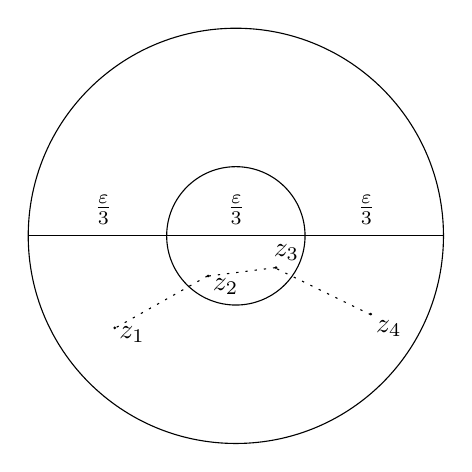
\begin{tikzpicture}[x=0.5pt,y=0.5pt,yscale=-1,xscale=1]
			%uncomment if require: \path (0,367); %set diagram left start at 0, and has height of 367
			
			%Shape: Circle [id:dp7038724886842289] 
			\draw   (270,171) .. controls (270,143.39) and (292.39,121) .. (320,121) .. controls (347.61,121) and (370,143.39) .. (370,171) .. controls (370,198.61) and (347.61,221) .. (320,221) .. controls (292.39,221) and (270,198.61) .. (270,171) -- cycle ;
			%Shape: Circle [id:dp20408854625505946] 
			\draw   (169.95,171) .. controls (169.95,88.13) and (237.13,20.95) .. (320,20.95) .. controls (402.87,20.95) and (470.05,88.13) .. (470.05,171) .. controls (470.05,253.87) and (402.87,321.05) .. (320,321.05) .. controls (237.13,321.05) and (169.95,253.87) .. (169.95,171) -- cycle ;
			%Straight Lines [id:da8755098905110549] 
			\draw    (169.95,171) -- (470.05,171) ;
			%Shape: Circle [id:dp34245043590360025] 
			\draw   (232,237.5) .. controls (232,237.22) and (232.22,237) .. (232.5,237) .. controls (232.78,237) and (233,237.22) .. (233,237.5) .. controls (233,237.78) and (232.78,238) .. (232.5,238) .. controls (232.22,238) and (232,237.78) .. (232,237.5) -- cycle ;
			%Shape: Circle [id:dp3226357363041006] 
			\draw   (299.5,200) .. controls (299.5,199.72) and (299.72,199.5) .. (300,199.5) .. controls (300.28,199.5) and (300.5,199.72) .. (300.5,200) .. controls (300.5,200.28) and (300.28,200.5) .. (300,200.5) .. controls (299.72,200.5) and (299.5,200.28) .. (299.5,200) -- cycle ;
			%Shape: Circle [id:dp8931755100052371] 
			\draw   (348.5,194) .. controls (348.5,193.72) and (348.72,193.5) .. (349,193.5) .. controls (349.28,193.5) and (349.5,193.72) .. (349.5,194) .. controls (349.5,194.28) and (349.28,194.5) .. (349,194.5) .. controls (348.72,194.5) and (348.5,194.28) .. (348.5,194) -- cycle ;
			%Shape: Circle [id:dp78063200787119] 
			\draw   (417,227.5) .. controls (417,227.22) and (417.22,227) .. (417.5,227) .. controls (417.78,227) and (418,227.22) .. (418,227.5) .. controls (418,227.78) and (417.78,228) .. (417.5,228) .. controls (417.22,228) and (417,227.78) .. (417,227.5) -- cycle ;
			%Straight Lines [id:da9144843916038057] 
			\draw  [dash pattern={on 0.84pt off 2.51pt}]  (299.5,200) -- (233,237.5) ;
			%Straight Lines [id:da2444506606827901] 
			\draw  [dash pattern={on 0.84pt off 2.51pt}]  (348.5,194) -- (300.5,200) ;
			%Straight Lines [id:da16195075964841843] 
			\draw  [dash pattern={on 0.84pt off 2.51pt}]  (417.5,228) -- (349,194.5) ;
			
			% Text Node
			\draw (312,140) node [anchor=north west][inner sep=0.75pt]    {$\frac{\varepsilon }{3}$};
			% Text Node
			\draw (406,140) node [anchor=north west][inner sep=0.75pt]    {$\frac{\varepsilon }{3}$};
			% Text Node
			\draw (216,140) node [anchor=north west][inner sep=0.75pt]    {$\frac{\varepsilon }{3}$};
			% Text Node
			\draw (234,234.9) node [anchor=north west][inner sep=0.75pt]    {$z_{1}$};
			% Text Node
			\draw (301.5,200) node [anchor=north west][inner sep=0.75pt]    {$z_{2}$};
			% Text Node
			\draw (345.5,175.4) node [anchor=north west][inner sep=0.75pt]    {$z_{3}$};
			% Text Node
			\draw (419.5,230.4) node [anchor=north west][inner sep=0.75pt]    {$z_{4}$};
		\end{tikzpicture}
	\end{center}
	Se $y \in f(B)$, allora esiste $x \in B$ tale che $y = f(x)$ e 
	\[ \norm{y- f_h(x)}_Y = \norm{f(x)-f_h(x)}_Y <\frac{\varepsilon}{3}. \]
	Inoltre, esiste $j =1,\dots,k$ tale che $f_h(x) \in \B(y_j,\frac{\varepsilon}{6})$, quindi $y \in C_j$, da cui 
	\[ f(B) \subseteq \bigcup_{j=1}^k C_j. \qedhere \]
\end{proof}
Nel corso di questa sezione, $E$ denoterà un sottoinsieme misurabile di $\R^n$.

\begin{definizione}
	Diciamo che un'applicazione $g : E \times \R^k \to \R$ è \emph{di Carathéodory} \index[analitico]{applicazione!di Carathéodory}, se valgono i seguenti fatti:
	\begin{enumerate}[$(a)$]
		\item per ogni $s \in \R^k$ l'applicazione $\left\lbrace x \mapsto g(x,s) \right\rbrace$ è misurabile su $E$,
		\item per \emph{q.o.} $x \in E$ l'applicazione $\left\lbrace s \mapsto g(x,s) \right\rbrace$ è continua su $\R^k$.
	\end{enumerate}
\end{definizione}
\begin{notazione}
	Data un'applicazione $u: E \to \R^k$, denotiamo con $g(x, u): E \to \R$ l'applicazione $\left\lbrace x \longmapsto g(x,u(x))\right\rbrace$.
\end{notazione}
\begin{teorema}\label{tecnicoperNemytskij}
	Se $g : E \times \R^k \to \R$ un'applicazione di Carathéodory, allora per ogni applicazione misurabile $u : E \to \R^k$, l'applicazione $g(x,u): E \to \R$ è
	misurabile.
	
	In particolare, se $u,v: E \to \R^k$ sono misurabili ed uguali \emph{q.o.} in $E$, anche $g(x, u)$ e $g(x, v)$ sono uguali \emph{q.o.} in $E$.
\end{teorema}
\begin{proof}
	Omettiamo la dimostrazione.
\end{proof}
\begin{teorema}\label{fondamentalepercontinuitàNemytskij}
	Sia $g: E \times \R^k \to \R$ un'applicazione di Carathéodory e siano $p_1,\dots, p_k,q \in \left[ 1,+\infty\right[$. Supponiamo che esistano $a \in L^q(E)$ e $b \in \R$ tali che
	\[ \abs{g(x,s_1,\dots,s_k)} \le a(x) + b\abs{s_1}^{\frac{p_1}{q}} + \dots + b\abs{s_k}^{\frac{p_k}{q}} \]
	per \emph{q.o.} $x \in E$ e per ogni $s \in \R^k$.
	Allora per ogni $u_1 \in L^{p_1}(E), \dots, u_k \in L^{p_k}(E)$ si ha $g(x,u_1,\dots , u_k) \in L^q(E)$ e l’applicazione $\mathcal{G}: L^{p_1}(E) \times \dots L^{p_k}(E) \to L^q(E)$ tale che
	\[ \mathcal{G}(u_1,\dots,u_k) = g(x,u_1,\dots,u_k) \]
	è continua.
\end{teorema}
\begin{proof}
	Siano $u_1 \in L^{p_1}(E),\dots ,u_k \in L^{p_k}(E)$. Per il Teorema \eqref{tecnicoperNemytskij}, $g(x, u_1, \dots, u_k)$ è ben definita, come classe di equivalenza, ed è misurabile.	
	
	Dal momento che
	\begin{align*}
		\abs{g(x,u_1,\dots,u_k)}^q &\le \left( a(x) + b\abs{u_1}^{\frac{p_1}{q}}+ \dots + b\abs{u_k}^{\frac{p_k}{q}}\right) \le \\
		&\le (k+1)^{q-1}\left( a(x)^q + b^q\abs{u_1}^{p_1}+ \dots + b^q\abs{u_k}^{p_k}\right), 
	\end{align*}
	risulta
	\[ \int_E \abs{g(x,u_1,\dots,u_k)}^q d \mathcal{L}^n \le (k+1)^{q-1} \left( \norm{a}^{q}_{L^{q}(E)} + b^q\norm{u_1}^{p_1}_{L^{p_1}(E)} +\dots + b^q\norm{u_k}^{p_k}_{L^{p_k}(E)}\right) .\]
	Ne segue $g(x,u_1,\dots,u_k) \in L^q(E)$.
	
	Sia ora, per $j = 1, . . . , k$, $(u_j^{(h)})$ una successione convergente ad $u_j$ in $L^{p_j}(E)$. Per ogni sottosuccessione $(u_j^{(h_l)})$, esistono una sottosuccessione $(u_j^{(h_{l_r})})$ e $w_j \in L^{p_j}(E)$ tali che
	\begin{align*}
		\lim\limits_{h} u_j^{(h_{l_r})}(x) &= u_j(x) \textup{ per q.o. } x \in E,\\
		\abs{u_j^{(h_{l_r})}} &\le w_j  \textup{ q.o. in }E.
	\end{align*}
	Per continuità di $g$, a meno di ulteriori sottosuccessioni,
	\begin{align*}
		\lim\limits_{h} g(x,u_1^{(h_{l_r})}(x),\dots,u_k^{(h_{l_r})}(x)) &= g(x,u_1(x),\dots,u(x)) \textup{ per q.o. } x \in E,\\
		\abs{g(x,u_1^{(h_{l_r})},\dots,u_k^{(h_{l_r})})}^q &\le (k+1)^{q-1} \left( a^q + b^qw_1^{p_1} + \dots + b^qw_k^{p_k} \right)  \textup{ q.o. in }E.
	\end{align*}
	e, per il Teorema della convergenza dominata,
	\[ \lim\limits_{m} \int_E \abs{g(x,u_1^{(h_{l_r})},\dots,u_k^{(h_{l_r})})- g(x,u_1,\dots,u_k)}^q d \mathcal{L}^n =0, \]
	ossia $g(x,u_1^{(h_{l_r})},\dots,u_k^{(h_{l_r})}) \to g(x,u_1,\dots,u_k)$ in $L^q(E)$. Allora $g(x,u_1^{(h)},\dots,u_k^{(h)}) \to g(x,u_1,\dots,u_k)$ in $L^q(E)$, ossia $\mathcal{G}$ è continua.
\end{proof}

\begin{definizione}
	Sia $g : E \times \R^k \to \R$ un'applicazione di Carathéodory. L'applicazione $\mathcal{G}: L^{p_1}(E) \times \dots L^{p_k}(E) \to L^q(E)$ tale che
	\[ \mathcal{G}(u_1,\dots,u_k) = g(x,u_1,\dots,u_k) \]
	si chiama \emph{operatore di Nemytskij}\index[analitico]{operatore!di Nemytskij}\index[simboli]{$\mathcal{G}$} o \emph{operatore di superposizione} associato a $g$.
\end{definizione}

Iniziamo dallo studio della continuità.
\begin{corollario}
	Siano $g : U \times (\R \times \R^n) \to \R$ un'applicazione di Carathéodory, $p \in \left[ 1,n\right[$ e $q \in \left[ 1,+\infty\right[ $. Supponiamo che esistano $a \in L^q(U)$ e $b \in \R$ tali
	che
	\[ \abs{g(x,s,\xi)} \le a(x) + b\abs{s}^{\frac{np}{(n-p)q}} + b\abs{\xi}^{\frac{p}{q}} \]
	per \emph{q.o.} $x \in U$ e per ogni $(s,\xi) \in \R \times \R^n$. Allora per ogni $u \in W^{1,p}_0(U)$ si ha $g(x, u, Du) \in L^q(U)$ e l’applicazione $\mathcal{T}: W^{1,p}_0(U) \to L^q(U)$ tale che
	\[ \mathcal{T}(u) = g(x,u,Du) \]
	è continua.
\end{corollario}
\begin{proof}
	Per il Teorema \eqref{fondamentalepercontinuitàNemytskij}, l'applicazione $\Psi_1: L^{\frac{np}{n-p}}(U) \times \left( L^p(U)\right) ^n \to L^q(U)$ tale che
	\[ \Psi_1(u,v_1,\dots,v_n) = g(x,u,v_1,\dots,v_n) \]
	è ben definita e continua. Inoltre, per ogni $j =1,\dots,n$ l'applicazione lineare $\Phi_j : W^{1,p}_0(U) \to L^p(U)$ tale che
	\[ \Phi_ju = D_ju \]
	è continua, infatti 
	\[ \norm{D_ju}_{L^p(U)} \le \norm{Du}_{L^p(U)} = \norm{u}_{W^{1,p}_0(U)}. \]
	Dal momento che, per la disuguaglianza di Poincaré, l'immersione $W^{1,p}_0(U) \hookrightarrow L^{\frac{np}{n-p}}(U)$ è continua, l'applicazione lineare $\Psi_2: W^{1,p}_0(U) \to L^{\frac{np}{n-p}}(U) \times \left( L^p(U)\right) ^n$ tale che
	\[ \Psi_2u = (u,D_1u,\dots,D_nu) \]
	è continua, infatti
	\[ \norm{\Psi_2u}_{L^{\frac{np}{n-p}}(U) \times \left( L^p(U)\right) ^n}^2  = \norm{u}_{L^{\frac{np}{n-p}}(U)}^2 + \norm{D_1u}^2_{L^p(U)} + \dots + \norm{D_nu}^2_{L^p(U)} \le C \norm{u}_{W^{1,p}_0(U)}^2. \]
	La tesi segue dal fatto che $\mathcal{T} = \Psi_1 \circ \Psi_2$.
\end{proof}

\begin{corollario}\label{continuitàNemytskij}
	Siano $g : U \times (\R \times \R^n) \to \R$ un'applicazione di Carathéodory, $p \in \left[ 1,n\right[$ e $q \in \left] \frac{n}{n-1},+\infty\right] $. Supponiamo che esistano $a \in L^{\frac{nq}{n+q}}(U)$ e $b \in \R$ tali
	che
	\[ \abs{g(x,s,\xi)} \le a(x) + b\abs{s}^{\frac{p(n+q)}{(n-p)q}} + b\abs{\xi}^{\frac{p(n+q)}{nq}} \]
	per \emph{q.o.} $x \in U$ e per ogni $(s,\xi) \in \R \times \R^n$. Allora per ogni $u \in W^{1,p}_0(U)$ si ha $g(x, u, Du) \in W^{-1,q}(U)$ e l’applicazione $\mathcal{T}: W^{1,p}_0(U) \to W^{-1,q}(U)$ tale che
	\[ \mathcal{T}(u) = g(x,u,Du) \]
	è continua.
\end{corollario}
\begin{proof}
	Per il Corollario precedente, l'applicazione $\Psi: W^{1,p}_0(U) \to L^{\frac{nq}{n+q}}(U)$ tale che
	\[ \Psi u = g(x,u,Du) \]
	è ben definita e continua. La tesi segue dunque dal fatto che, per la disuguaglianza di Poincaré duale, l'immersione $ L^{\frac{nq}{n+q}}(U) \hookrightarrow W^{-1,q}(U)$ è continua.
\end{proof}
\begin{osservazione}
	Il Corollario \eqref{continuitàNemytskij} appena dimostrato vale, in particolare, per $q = p'$.
\end{osservazione}

Affrontiamo ora lo studio della compattezza.

\begin{teorema}\label{compattezzaNemytskij}
Siano $g : U \times (\R \times \R^n) \to \R$ un'applicazione di Carathéodory, $p \in \left[ 1,n\right[$ e $q \in \left] \frac{n}{n-1},+\infty\right] $. Supponiamo che per ogni $\varepsilon>0$ esista $a_\varepsilon \in L^{\frac{nq}{n+q}}(U)$ tale che 
	\[ \abs{g(x,s,\xi)} \le a_\varepsilon(x) + \varepsilon\abs{s}^{\frac{p(n+q)}{(n-p)q}} + \varepsilon \abs{\xi}^{\frac{p(n+q)}{nq}} \]
per \emph{q.o.} $x \in U$ e per ogni $(s,\xi) \in \R \times \R^n$. Allora l’applicazione $\mathcal{T}: W^{1,p}_0(U) \to W^{-1,q}(U)$ tale che
\[ \mathcal{T}(u) = g(x,u,Du) \]
è continua e compatta.
\end{teorema}
\begin{proof}
La continuità segue dal Corollario \eqref{continuitàNemytskij}.

Vediamo, innanzitutto, il caso in cui esistono $R>0$ ed $a \in L^\infty(U)$ tali che 
\[ \abs{g(x,s,\xi)} \le a(x) \textup{ per q.o. } x \in U \textup{ ed ogni } (s,\xi) \in \R \times \R^n, \]
\[ a(x) = 0 \textup{ per q.o. } x \in U \setminus \B(0,R). \]
Consideriamo $(u_h)$ in $W^{1,p}_0(U)$ limitata. Siccome
\[ \norm{g(x,u_h,Du_h)}^q_{L^q(U)} \le \norm{a}_{L^\infty(U)}^q\mathcal{L}^n(\B(0,R)) <+\infty, \]
allora $(g(x,u_h,Du_h))$ è limitata in $L^q(U)$ e $g(x,u_h,Du_h) = 0$ q.o. in $U\setminus \B(0,R)$. Sia $\vartheta \in C^\infty_c(\B(0,R+1))$ tale che $0\le \vartheta \le 1$ e $\vartheta = 1$ in $\overline{\B(0,R)}$.

Per la Proposizione \eqref{Rellichsottosteroididuale}, a meno di sottosuccessioni, $(g(x,u_h,Du_h))$ converge in $W^{-1,q}(U \cap \B(0,R+1))$, quindi è di Cauchy in $W^{-1,q}(U \cap \B(0,R+1))$. Per ogni $v \in W^{1,q'}_0(U)$ si ha che $\vartheta v \in W^{1,q'}_0(U\cap B(0,R+1))$, quindi, per la disuguaglianza di Poincaré,
\begin{align*}
&\abs*{\int_U (g(x,u_h,Du_h)- g(x,u_k,Du_k))vd\mathcal{L}^n} = \abs*{\int_{U \cap \B(0,R)}\hspace{-25pt} (g(x,u_h,Du_h)- g(x,u_k,Du_k))vd\mathcal{L}^n} = \\
&= \abs*{\int_{U \cap \B(0,R)}\hspace{-25pt} (g(x,u_h,Du_h)- g(x,u_k,Du_k))\vartheta vd\mathcal{L}^n} = \\
&= \abs*{\int_{U \cap \B(0,R+1)}\hspace{-35pt} (g(x,u_h,Du_h)- g(x,u_k,Du_k))\vartheta vd\mathcal{L}^n} \le \\
&\le \norm{g(x,u_h,Du_h)- g(x,u_k,Du_k)}_{W^{-1,q}(U\cap \B(0,R+1))} \norm{\vartheta v}_{W^{1,q'}_0(U\cap \B(0,R+1))} \le \\
&\le C\norm{g(x,u_h,Du_h)- g(x,u_k,Du_k)}_{W^{-1,q}(U\cap \B(0,R+1))}\norm{v}_{W^{1,q'}_0(U)},
\end{align*}
da cui
\begin{align*}
&\norm{g(x,u_h,Du_h)- g(x,u_k,Du_k)}_{W^{-1,q}(U)} \le  \\
&\le C\norm{g(x,u_h,Du_h)- g(x,u_k,Du_k)}_{W^{-1,q}(U\cap \B(0,R+1))}
\end{align*}
per cui $(g(x,u_h,Du_h))$ è di Cauchy in $W^{-1,q}(U)$, quindi convergente.

Vediamo ora il caso in cui esista $a \in L^{\frac{nq}{n+q}}(U)$ tale che 
\[ \abs{g(x,s,\xi)} \le a(x) \textup{ per q.o. } x \in U \textup{ ed ogni } (s,\xi) \in \R\times \R^n. \]
Consideriamo 
\[ g_h(x,s,\xi) = \begin{cases}
	g(x,s,\xi) & \textup{se } a(x) \le h \textup{ e } \abs{x}<h,\\
	0 & \textup{ altrimenti},
\end{cases} \]
e 
\[ a_h(x) = \begin{cases}
	a(x) & \textup{se } a(x) \le h \textup{ e } \abs{x}<h,\\
	0 & \textup{ altrimenti},
\end{cases} \]
Evidentemente $g_h$ è di Carathéodory e 
\[ \abs{g_h(x,s,\xi)} \le a_h(x) \textup{ per q.o. } x \in U \textup{ ed ogni } (s,\xi) \in \R\times \R^n. \]
Allora, per il passo precedente, l'applicazione $\mathcal{T}_h: W^{1,p}_0(U) \to W^{-1,q}(U)$ tale che
\[ \mathcal{T}_h(u) = g_h(x,u,Du) \]
è continua e compatta. Siccome per ogni $u \in W^{1,p}_0(U)$ si ha
\[ \int_U \abs{g(x,u,Du) - g_h(x,u,Du)}^{\frac{nq}{n+q}}d\mathcal{L}^n \le \int_U a^{\frac{nq}{n+q}}(1-\chi_{\left\lbrace x \in \R^n: a(x)\le h\right\rbrace}\chi_{\B(0,h)})d\mathcal{L}^n. \]
Dal Teorema della convergenza dominata, si deduce che per ogni $B \subseteq W^{1,p}_0(U)$ limitato,
\[ \lim\limits_{h} \underset{u \in B}{\sup}\; \norm{g_h(x,u,Du) -g(x,u,Du)}_{L^{\frac{nq}{n+q}}(U)} = 0.  \]
Per la Disuguaglianza di Poincaré duale, 
\[ \lim\limits_{h} \underset{u \in B}{\sup}\; \norm{g_h(x,u,Du) -g(x,u,Du)}_{W^{-1,q}(U)} = 0,  \]
che, combinata con il Lemma \eqref{compattezzaelimitiuniformi}, da la compattezza desiderata.

Nel caso generale, per $\varepsilon = \frac{1}{h}$, con $h \in N\setminus\left\lbrace 0\right\rbrace$, esiste $a_h \in L^{\frac{nq}{n+q}}(U)$ tale che 
	\[ \abs{g(x,s,\xi)} \le a_h(x) + \frac{1}{h}\abs{s}^{\frac{p(n+q)}{(n-p)q}} + \frac{1}{h} \abs{\xi}^{\frac{p(n+q)}{nq}} \]
per q.o. $x \in U$ e per ogni $(s,\xi) \in \R \times \R^n$. Poniamo 
\[ g_h(x,s,\xi) = \min \left\lbrace \max\left\lbrace g(x,s,\xi),-a_h(x)\right\rbrace a_h(x)\right\rbrace.  \]
Evidentemente $ g_h$ è di Carathéodory e 
\[ \abs{g_h(x,s,\xi)} \le a_h(x) \textup{ per q.o. } x \in U \textup{ ed ogni } (s,\xi) \in \R\times \R^n. \]
Allora, per il passo precedente, l'applicazione $\mathcal{T}_h: W^{1,p}_0(U) \to W^{-1,q}(U)$ tale che
\[ \mathcal{T}_h(u) = g_h(x,u,Du) \]
è continua e compatta. Osservando che 
\[ \abs{g(x,s,\xi) - g_h(x,s,\xi)} \le \frac{1}{h}\abs{s}^{\frac{p(n+q)}{(n-p)q}} + \frac{1}{h} \abs{\xi}^{\frac{p(n+q)}{nq}} \]
per q.o. $x \in U$ e per ogni $(s,\xi) \in \R \times \R^n$, per ogni $u \in W^{1,p}_0(U)$ si ha
\[ \int_U \abs{g(x,s,\xi) - g_h(x,s\xi)}^{\frac{nq}{n+q}} d\mathcal{L}^n \le 2^{\frac{nq-n-q}{n+q}}\left(\frac{1}{h} \right)^{\frac{nq}{n+q}} \left(\int_U \abs{u}^\frac{np}{n-p} d\mathcal{L}^n + \int_U \abs{Du}^p d\mathcal{L}^n \right)  \]
e, per la disuguaglianza di Poincaré,
\[ \int_U \abs{g(x,s,\xi) - g_h(x,s\xi)}^{\frac{nq}{n+q}} d\mathcal{L}^n \le C \left(\frac{1}{h} \right)^{\frac{nq}{n+q}}\left( \norm{u}_{W^{1,p}_0(U)}^{\frac{np}{n-p}} + \norm{u}_{W^{1,p}_0(U)}^p\right).   \]
Pertanto per ogni $B \subseteq W^{1,p}_0(U)$ limitato si ha
\[ \lim\limits_{h} \underset{u \in B}{\sup}\; \norm{g_h(x,u,Du) -g(x,u,Du)}_{L^{\frac{nq}{n+q}}(U)} = 0.  \]
Per la Disuguaglianza di Poincaré duale, 
\[ \lim\limits_{h} \underset{u \in B}{\sup}\; \norm{g_h(x,u,Du) -g(x,u,Du)}_{W^{-1,q}(U)} = 0,  \]
che, in combinazione con il Lemma \eqref{compattezzaelimitiuniformi}, da la compattezza desiderata.
\end{proof}

\begin{osservazione}
	Il Teorema \eqref{compattezzaNemytskij} appena dimostrato vale, in particolare, per $q = p'$. In questo caso la stima di crescita su $g$ assume la forma
		\[ \abs{g(x,s,\xi)} \le a_\varepsilon(x) + \varepsilon\abs{s}^{\frac{n(p-1)+p}{n-p}} + \varepsilon \abs{\xi}^{\frac{n(p-1)+p}{n}}. \]
\end{osservazione}

\begin{osservazione}
E opportuno confrontare la condizione di crescita del Teorema \eqref{compattezzaNemytskij} con quella del Corollario \eqref{continuitàNemytskij}. Gli esponenti $\frac{p(n+q)}{(n-p)q}$ e $\frac{p(n+q)}{nq}$ rappresentano gli andamenti critici con cui si può garantire la continuità, ma non la completa continuità dell’operatore. Non appena si rimane al di sotto di tali crescite, come nel Teorema \eqref{compattezzaNemytskij}, si ottiene la completa continuità dell’operatore. Non occorre invece imporre una diversa
sommabilità sul termine $a_\varepsilon$. Si osservi anche che nel Teorema \eqref{compattezzaNemytskij} non viene fatta alcuna ipotesi sull’aperto $U$.
In particolare, non si richiede che $U$ sia limitato.
\end{osservazione}

\begin{corollario}
Siano $g : U \times (\R \times \R^n) \to \R$ un'applicazione di Carathéodory, $p \in \left[ 1,n\right[$ e $q \in \left] \frac{n}{n-1},+\infty\right] $. Supponiamo $\mathcal{L}^n(U)<+\infty$ e che esistano $a \in L^{\frac{nq}{n+q}}(U)$, $b \in \R$, $r_0 \in \left[ 1,\frac{p(n+q)}{(n-p)q}\right[$ e $r_1 \in \left[ 1,\frac{p(n+q)}{nq}\right[$  tali che 
\[ \abs{g(x,s,\xi)} \le a(x) + b\abs{s}^{r_0} + b \abs{\xi}^{r_1} \]
per \emph{q.o.} $x \in U$ e per ogni $(s,\xi) \in \R \times \R^n$. Allora l’applicazione $\mathcal{T}: W^{1,p}_0(U) \to W^{-1,q}(U)$ tale che
\[ \mathcal{T}(u) = g(x,u,Du) \]
è continua e compatta.
\end{corollario}
\begin{proof}
Ricordiamo che, per la Disuguaglianza di Young pesata, per ogni $\alpha \in \left] 1,+\infty\right[, s,t \in \R$ ed $\varepsilon >0$ si ha
\[ \abs{st} \le \varepsilon \abs{s}^{\alpha} + \frac{\alpha-1}{\alpha^{\frac{\alpha}{\alpha-1}}\varepsilon^{\frac{1}{\alpha -1}}}\abs{t}^{\alpha'}. \]
Scelti 
\begin{align*}
	\alpha &= \frac{p(n+q)}{(n-p)qr_0}, & \beta &=\frac{p(n+q)}{(nqr_1},
\end{align*}
per ogni $\varepsilon > 0$ risulta
\[ \abs{g(x,s,\xi)} \le a(x) + \frac{\alpha -1}{\alpha^{\frac{\alpha}{\alpha-1}}\varepsilon^{\frac{1}{\alpha -1}}}b^{\alpha'} + \frac{\beta -1}{\beta^{\frac{\beta}{\beta-1}}\varepsilon^{\frac{1}{\beta -1}}}b^{\beta'} + \varepsilon\abs{s}^{\frac{p(n+q)}{(n-p)q}} + \varepsilon \abs{\xi}^{\frac{p(n+q)}{nq}}. \]
D’altronde, avendo $U$ misura finita, ogni funzione costante appartiene a $L^{\frac{nq}{n+q}}(U)$. La tesi discende allora dal Teorema \eqref{compattezzaNemytskij}.
\end{proof}

\begin{osservazione}
	Il Corollario appena dimostrato vale, in particolare, per $q = p'$.
\end{osservazione}